\documentclass[applsci,article,accept,pdftex,moreauthors]{Definitions/mdpi} 
% \documentclass[preprints,article,submit,pdftex,moreauthors]{Definitions/mdpi} 
% For posting an early version of this manuscript as a preprint, you may use "preprints" as the journal.
% Changing "submit" to "accept" before posting will remove line numbers.
% Instead of applsci, for a general submission, use "preprints".

% ==================================================

% MDPI internal commands - do not modify
\firstpage{1} 
\makeatletter 
\setcounter{page}{\@firstpage} 
\makeatother
\pubvolume{1}
\issuenum{1}
\articlenumber{0}
\pubyear{2025}
\copyrightyear{2025}
\externaleditor{ } % More than 1 editor, please add `` and '' before the last editor name
\datereceived{3 February 2025} 
\daterevised{25 February 2025} % Comment out if no revised date
\dateaccepted{26 February 2025} 
\datepublished{ } 
% \datecorrected{} % For corrected papers: "Corrected: XXX" date in the original paper.
% \dateretracted{} % For retracted papers: "Retracted: XXX" date in the original paper.
\hreflink{https://doi.org/} % If needed use \linebreak
% \doinum{}
% \pdfoutput=1 % Uncommented for upload to arXiv.org
% \CorrStatement{yes} % For updates
% \longauthorlist{yes} % For many authors that exceed the left citation part

% ==================================================

% Add packages and commands here. The following packages are loaded in our class file: fontenc, inputenc, calc, indentfirst, fancyhdr, graphicx, epstopdf, lastpage, ifthen, float, amsmath, amssymb, lineno, setspace, enumitem, mathpazo, booktabs, titlesec, etoolbox, tabto, xcolor, colortbl, soul, multirow, microtype, tikz, totcount, changepage, attrib, upgreek, array, tabularx, pbox, ragged2e, tocloft, marginnote, marginfix, enotez, amsthm, natbib, hyperref, cleveref, scrextend, url, geometry, newfloat, caption, draftwatermark, seqsplit
% cleveref: load \crefname definitions after \begin{document}



\usepackage[utf8]{inputenc}
\usepackage{color}
\usepackage{graphicx}
\usepackage{placeins}
% \usepackage[margin=1in]{geometry}
\usepackage{appendix}
\usepackage{amsmath, amssymb, bm}
\usepackage{multirow}
\usepackage{placeins}
\usepackage{xfrac}
% \usepackage[colorlinks=true, linkcolor=blue, citecolor=blue]{hyperref}
% \usepackage[nameinlink, capitalize]{cleveref}
\usepackage[font=footnotesize, labelfont=bf]{caption}
%\usepackage{subcaption}
\usepackage[version=4]{mhchem}
\usepackage{lineno}
\usepackage{bm}
\usepackage{comment}
\usepackage[T1]{fontenc}
\usepackage{anyfontsize}
\usepackage[labelformat=simple]{subfig}
\renewcommand\thesubfigure{\normalfont(\textbf{\alph{subfigure}})}

\newcommand{\?}{\stackrel{?}{=}}

% ==================================================

% Full title of the paper (Capitalized)
\Title{Atomistic Investigation of Plastic Deformation and Dislocation Motion in Uranium \colorbox{green}{Mononitride}}%MDPI: Important note:
%1. The paper was edited by our English editor, please check the whole text and confirm if your meaning is retained.
%2. Do not delete any comment we left for you and reply to each comment so that we can understand your meaning clearly.
%3. Please directly correct on this version. If you need to revise somewhere in your paper, please highlight the revisions and track changes to make us known.
%4. Please finish the proofreading based on this version.
%5.Please confirm and revise all the comments with “Confirmed”, “OK”, “Revised”, “It should be italic”; “I confirm”; “I confirm xx is correct”; “I have checked and revised all.” , etc.“
%6. Please note that at this stage (the manuscript has been accepted in the current form), we will not accept authorship or content changes to the main text.
%(Thank you for your cooperation in advance.)
%BB: all comments and highlights have been addressed


% MDPI internal command: Title for citation in the left column
\TitleCitation{Atomistic Investigation of Plastic Deformation and Dislocation Motion in Uranium Mononitride}

% Author Orchid ID: enter ID or remove command
\newcommand{\orcidauthorA}{0009-0009-5882-3345} % Add \orcidA{} behind the author's name
\newcommand{\orcidauthorB}{0000-0003-1964-1177} % Add \orcidB{} behind the author's name
\newcommand{\orcidauthorC}{0000-0002-4158-0123} % Add \orcidC{} behind the author's name

% Authors, for the paper (add full first names)
\Author{\hl{Mohamed} %MDPI: Please carefully check the accuracy of names and affiliations.
 \hl{AbdulHameed} %MDPI: Please confirm if the format of the last name is correct, or a space should be added as “Abdul Hameed”. %BB: Name is correct, no space.
 $^{1}$\orcidA{}, Benjamin Beeler $^{1,2,*}$\orcidB{} and Antoine Claisse $^{3}$\orcidC{}}

% \longauthorlist{yes}

% MDPI internal command: Authors, for metadata in PDF
\AuthorNames{Mohamed AbdulHameed, Benjamin Beeler and Antoine Claisse}

\AuthorCitation{AbdulHameed, M.; Beeler, B.; Claisse, A.}

% Affiliations / Addresses (Add [1] after \address if there is only one affiliation.)
\address{%
$^{1}$ \quad Department of Nuclear Engineering, North Carolina State University, Raleigh, NC 27695, USA; \hl{maabdulh@ncsu.edu} %MDPI: The email addresses were added according to those submitted online at susy.mdpi.com. Please confirm. %BB: Confirmed
\\
$^{2}$ \quad \hl{Idaho National Laboratory}%MDPI: Please confirm if the address information is complete. %BB: Confirmed
, Idaho Falls, ID 83415, USA\\
$^{3}$ \quad Westinghouse Electric Sweden, \hl{SE} %MDPI: Please confirm if “SE” is a part of the postal code and is necessary to be retained. %BB: SE is part of the postal code.
 72163 \hl{Vasteras}%MDPI: English writing is recommended. Please confirm the revision. %BB: The name of the city is in Swedish, thus we would recommend using the Swedish spelling/text. 
, Sweden; \hl{claissaj@westinghouse.com}}

% Contact information of the corresponding author
\corres{Correspondence: bwbeeler@ncsu.edu}

\abstract{Uranium mononitride (UN) is a promising advanced nuclear fuel due to its high thermal conductivity and high fissile density. However, many aspects of its mechanical behavior, particularly at reactor-relevant conditions, remain unclear. In this study, molecular dynamics (MD) simulations were employed to investigate the deformation behavior and dislocation motion in UN. We found that the Kocevski potential predicts the principal slip system as $\frac{1}{2} \langle 110 \rangle \{110\}$, aligning with experimental data. On the other hand, the Tseplyaev potential predicts slip to primarily occur on $\frac{1}{2} \langle 110 \rangle \{111\}$. MD simulations of stress--strain behavior were used to estimate the nanoindentation hardness, revealing that the Kocevski potential accurately predicts hardness even though it fails to model dynamic plasticity. Complete dislocation mobility functions have been fitted for the edge and screw dislocations in both the thermally activated and phonon-drag regimes. The 300 K linear mobility of the edge dislocation using the Tseplyaev potential was found to be 817 $\mathrm{Pa}^{-1} \! \cdot \! \mathrm{s}^{-1}$, whereas that of the screw dislocation using the Kocevski potential was found to be 4546 $\mathrm{Pa}^{-1} \! \cdot \! \mathrm{s}^{-1}$. At intermediate stresses, we observed that the subsonic steady-state motion of the edge dislocation in UN is intermittently interrupted by velocity jumps, reaching the average sound velocity. Finally, the threshold Schmid stress is calculated as 179--197 MPa, which gives an upper-limit estimate of the uniaxial yield stress of polycrystalline UN of 548--603 MPa. These findings, including the fitted dislocation mobility function, provide essential input for future plasticity and dislocation dynamics models of nuclear fuels.}

% Keywords
\keyword{uranium nitride; molecular dynamics; plastic deformation; Peierls stress; dislocation mobility} 

% ==================================================

% Only for the journal Applied Sciences
% \featuredapplication{Authors are encouraged to provide a concise description of the specific application or a potential application of the work. This section is not mandatory.}

% ==================================================

\begin{document}

\section{Introduction}

Uranium mononitride (UN) is a promising advanced nuclear fuel due to its many attractive characteristics including a high uranium density, high thermal conductivity, good chemical compatibility with most potential cladding materials, and~long fuel residence time~\cite{Ekberg2018, Wallenius2020, Uno2020}. However, it suffers from some drawbacks including complicated fabrication processes, high fuel cost owing to the need for $^{15}$N enrichment, and~low resistance to oxidation by high-temperature steam~\cite{Ekberg2018, Wallenius2020, Uno2020}. Many aspects of the behavior of UN under high temperatures and/or irradiation are lacking in both consistent experimental data and detailed mechanistic understanding. The~mechanical properties of nuclear fuels are crucial for a better understanding of the pellet-cladding mechanical interaction (PCMI) that occurs during reactor operation. The~mechanical aspects relevant to PCMI in UN include deformation behavior (stress--strain) and dislocation properties. These mechanical properties significantly influence its behavior under high temperatures and high radiation intensity. Specifically, the~deformation behavior affects the material's ability to accommodate thermal expansion and fission gas swelling, impacting the integrity of the fuel-cladding gap and influencing PCMI~\cite{Olander2017, Olander2021}. Additionally, dislocation interactions with radiation-induced defects can alter the material's creep behavior and stress relaxation mechanisms at elevated temperatures, potentially leading to enhanced deformation or cracking under operational conditions~\cite{Olander2017, Olander2021}. Therefore, a~detailed understanding of the mechanical properties of UN is essential for predicting its performance and ensuring its reliability as a nuclear~fuel.

% Stress-strain behavior and dislocations

Molecular dynamics (MD) simulations of deformation behavior have been conducted for many materials including silicon (Si) and silicon carbide (SiC) \cite{Ivashchenko2007}, aluminum~\cite{Li2020}, and~copper~\cite{Hansson2022}. Due to the size limitation of MD simulations, most of these studies are of a descriptive nature, except~for those studies that specifically target nanomaterial applications and for which the MD size is representative. To~the best of our knowledge, no computational studies of the stress--strain behavior of UN exist in the open literature. The~only experimental study found in the literature on the deformation behavior in UN is by Sole and van der Walt~\cite{Sole1968}. They observed that the majority of slip traces on UN samples exist within the $\{110\}$ planes, which implies that $\frac{1}{2} \langle 110 \rangle \{110\}$ (with angle brackets referring to the slip direction and curly brackets referring to the slip plane) are the primary slip planes in UN. They also report that most of the dislocations observed are nearly pure screw dislocations. A~secondary slip system along the $\{112\}$ planes has been observed by the authors, who hypothesized a process for its occurrence that is based on the reaction of two screw dislocations to form an edge dislocation confined to the (112) plane. However, the~mechanism by which this edge dislocation slips remains~unclear.

Another study was conducted on dislocations in UN by Xiu~et~al. \cite{Xiu2021}, who investigated dislocation loops in a proton-irradiated uranium--nitrogen--oxygen system. They stated that only $\frac{1}{2} \langle 110 \rangle$ dislocation loops can be observed in the UN phase. They also conducted 0~K molecular statics using the Tseplyaev and Starikov angular-dependent potential~\cite{Tseplyaev2016} to determine the formation energies of $\frac{1}{2} \langle 110 \rangle$ and $\frac{1}{3} \langle 111 \rangle$ dislocation loops at various loop sizes. However, as~shown previously~\cite{AbdulHameed2024} and verified in this study, 0 K calculations using the Tseplyaev and Starikov angular-dependent potential~\cite{Tseplyaev2016} of defective UN structures can be trapped at metastable states and should be treated~cautiously. 

Nucleation of dislocations is a primary product of radiation damage in nuclear materials. Knowledge of dislocation mobility is essential to model glide-controlled creep accurately~\cite{Skelton2017}. Osetsky and Bacon~\cite{Osetsky2003} introduced a fully atomistic formalism to calculate the Peierls stress and applied it to straight edge dislocations in body-centered cubic iron. Alternatively, a~hybrid continuum--atomistic approach based on the Peierls--Nabarro theory was used by Liu~et~al. \cite{Liu2012} to calculate the Peierls stresses and core widths for sodium chloride (NaCl) and lithium fluoride (LiF) and by Skelton and Walker~\cite{Skelton2017} to calculate the same parameters for uranium dioxide (\ce{UO2}). Many studies have looked at the dislocation mobility in metals like aluminum~\cite{Cho2017, Dang2019} and nickel~\cite{Olmsted2005}, as~well as in aluminum--magnesium alloys~\cite{Olmsted2005} and steels~\cite{Kaloni2023}. Additionally, Yadav~et~al. \cite{Yadav2014} conducted a density functional theory (DFT) study of dislocations in titanium nitride and determined the principal slip system. Ukita~et~al. \cite{Ukita2018} conducted a similar DFT study for NaCl as well as silver~chloride.

Two promising interatomic potentials of UN exist in the literature: Tseplyaev and Starikov's angular-dependent potential~\cite{Tseplyaev2016}, and~Kocevski~et~al.'s embedded-atom method (EAM) potential~\cite{Kocevski2022II}. Both potentials have been assessed in our previous work~\cite{AbdulHameed2024}, where their effectiveness in predicting thermophysical and mechanical properties was evaluated, identifying their strengths and weaknesses. Notably, while these potentials showed some capability in predicting mechanical properties and defect formation energies, their suitability for modeling dynamic phenomena remained uncertain. Given the importance of understanding plastic deformation in nuclear fuels, further investigation is needed into their ability to capture key dynamical processes, such as dislocation slip and mobility, using simplified single-crystal models. This is particularly valuable since such models usually provide a baseline to develop a multi-scale modeling approach that can predict the macroscopic mechanical behavior of polycrystalline samples from elementary atomistic~mechanisms.

In this work, we perform MD simulations of the stress--strain behavior of nanocrystalline UN, investigating the dynamic processes of plastic deformation and identifying the principal slip systems. The~Peierls stress, threshold Schmid stress, and~dislocation mobility are computed for straight edge and screw dislocations in UN, with~complete mobility functions fitted. Finally, the~yield stress is estimated based on two different approaches. In~conducting these simulations, we carefully account for the limitations identified in our previous study~\cite{AbdulHameed2024}, ensuring that the weaknesses of each potential are avoided---such as not relying on 0 K energy minimizations with the Tseplyaev potential and circumventing structures that invoke excessive U-U repulsion with the Kocevski~potential.

\section{Computational~Methods}

All MD calculations performed in this work utilize the Large-scale Atomic/Molecular Massively Parallel Simulator (LAMMPS) \colorbox{green}{software package (Version 2 August 2023)} %MDPI: Please state the software version number, including the following highlight. %BB: Corrected
 \cite{Thompson2022} with a time step of 1 fs and the Tseplyaev~\cite{Tseplyaev2016} and Kocevski~\cite{Kocevski2022II} potentials. The~Open Visualization Tool (OVITO) \colorbox{green}{software package (Version 3.10.6)}~\cite{Stukowski2010} is used for supercell visualization and~analysis.

\subsection{Deformation~Behavior}

In this paper, we investigate the stress--strain behavior of UN single crystals at \mbox{$T$ = 300 K} and strain rates of $10^8$, $5 \times 10^8$, and~$10^9$ s$^{-1}$ using both the Tseplyaev and Kocevski potentials. Due to computational limitations, MD simulations of uniaxial tension are limited to nanometer-sized supercells and strain rates of at least $10^7$ s$^{-1}$ \cite{Lao2013}. $150 \times 30 \times 30$ UN supercells are first equilibrated at 300 K and zero pressure for 100 ps using a Nosé--Hoover thermostat--barostat. After~equilibration, the~load is applied in the [100] direction at the target strain rate, and~the material is allowed to deform in the isothermal--isobaric (\textit{NPT}) ensemble up to fracture. Periodic boundary conditions (PBCs) are applied in all directions throughout the whole simulation. Relaxation is conducted such that the $x$-, $y$-, and~$z$-directions are independent, but~the supercell remains orthogonal. Note that during deformation, the~$x$-direction is controlled by the strain~rate.

To estimate the nanoindentation hardness, we perform deformation simulations at strain rates of $10^7$, $10^8$, and~$10^9$ s$^{-1}$ but with PBCs applied only along the loading direction, i.e.,~the $x$-axis, whereas surfaces perpendicular to the $y$- and $z$-axes are modeled with fixed boundary conditions, yielding free surfaces along these planes. Before~deformation, the~supercells are equilibrated in the \textit{NPT} ensemble for 50 ps (where the pressure is allowed to equilibrate only along the $x$-axis), and~then in the canonical (\textit{NVT}) ensemble for a further 50 ps. Uniaxial tension is then applied in the \textit{NVT} ensemble until fracture. From~the stress--strain curves of nanocrystalline samples with free surfaces, the~nanoindentation hardness can be estimated by measuring the stress--strain curves at different strain rates, ($\Dot\epsilon$)\hl{,} %MDPI: Please check if the format of this variable is correct. %BB: Variable format has been corrected
 \textls[-15]{recording the maximum stress, $\sigma_\mathrm{max}$, for~each case, and~then extrapolating $\sigma_\mathrm{max}(\Dot{\epsilon})$ to $\Dot{\epsilon} \rightarrow 0$ \cite{Ivashchenko2007}.} The~linearly extrapolated value should correspond to the experimental nanoindentation hardness~values.

We define the maximum stress in the deformation process as the yield stress. Young's modulus is obtained by fitting the linear part of the stress--strain curve excluding the transient at the origin and the nonlinearities near the yield point. The~Young's modulus along the [100] direction can also be calculated from the elastic constants according to the following \hl{formula} %MDPI: 1. Please confirm whether there are repeated formulas in paper. 2. The format of the formulas needs to be consistent. Please check/confirm %BB: No repeated formulas. Formula format is consistent. 
~\cite{Rosler2007}:
\begin{equation}
E_{\langle 100 \rangle} = \frac{(C_{11}-C_{12}) \times (C_{11}+2 C_{12})}{C_{11}+C_{12}}
\label{Eq:E100}
\end{equation}

% Also, the anisotropy factor is calculated from~\cite{Meyers2009}:
% \begin{equation}
% A = \frac{2 C_{44}}{C_{11} - C_{12}}
% \label{Eq:A}
% \end{equation}

To monitor structural development during deformation, the~centrosymmetry parameter (CSP) was calculated by OVITO for snapshots of the simulated supercells using the minimum-weight matching algorithm~\cite{Larsen2020}. The~CSP is a measure of the lattice disorder and is defined according to~\cite{Kelchner1998}\hl{} %MDPI: 1. Please confirm if all bolds of variables are necessary and should be retained. 2. The format of the same variables in the texts and equations should be consistent (italic, bold, case, superscript and subscript ...). Please check throughout the manuscript if they are correct. %BB: variables should be bolded and this format is retained in the text.

\begin{equation}
\mathrm{CSP} = \sum_{i=1}^{N/2} |\mathbf{r}_i + \mathbf{r}_{i+N/2}|^{2} 
\end{equation}
where $N$ is the number of nearest neighbors surrounding an atom ($N$ = 6 for the NaCl crystal structure), and~$\mathbf{r}_i$ and $\mathbf{r}_{i+N/2}$ are two vectors from the atom under consideration to a pair of opposite neighbor atoms. For~an ideally centrosymmetric crystal, the~contributions of all neighbor pairs cancel, and~the resulting CSP is zero. The~CSP algorithm is robust against thermal fluctuations; for a single crystal, it shows a single peak that starts at zero and whose width increases with increasing $T$. A~second peak in the CSP plot corresponds to a different local environment, e.g.,~dislocations and highly disordered grain boundaries (GBs) \cite{Bulatov2006, Larsen2020}. The~CSP has dimensions of squared distance and is usually given in units of $a^2$, where $a$ is the lattice parameter. The~CSP algorithm is an indirect characterization technique. To~directly visualize and analyze dislocations, OVITO's dislocation extraction algorithm (DXA) \cite{Stukowski2012} is utilized and~applied to the U sublattice. A~limitation of the DXA is that it can only identify predefined dislocations in single-component crystals, so that dislocations with a Burgers vector that does not belong to any of the predefined families are not identified. This prohibits the algorithm from identifying GB dislocations that have much shorter Burgers vectors than those of lattice dislocations~\cite{Cai2016}. Since each sublattice in the B1 structure of UN is a face-centered cubic (FCC) lattice, by~applying the DXA to the U sublattice we can accurately visualize~dislocations. 

\subsection{Dislocation~Motion}

Ionic crystals have a Burgers vector $\mathbf{b} = \frac{1}{2} \langle 110 \rangle$ and four possible slip planes, $\{ 110 \}$, $\{ 111 \}$, $\{ 100 \}$, and~$\{ 112 \}$, with the principal one being determined mainly by the bonding nature~\cite{Hull2011, Yadav2014}. Three straight edge dislocations are studied in this paper: $\frac{1}{2} [ 110 ] ( 1 \Bar{1} 0 )$, $\frac{1}{2} [ \Bar{1} 1 0 ] ( 111 )$, and~$\frac{1}{2} [ \Bar{1} 10 ] ( \Bar{1} \Bar{1} 2 )$, where their Burgers vectors are along the $x$-axis and line vectors along the $z$-axis. To~construct an edge dislocation, two half-crystals are stacked on top of one another---the top half-crystal containing one extra atomic plane compared to the bottom half-crystal. Then, strains of $-0.5~b/l_x$ and $+0.5~b/l_x$ are applied to the top and bottom crystals, respectively, with $l_x$ being the length of the respective half-crystal along the $x$-axis~\cite{Osetsky2003}. That is, the~top half-crystal is compressed by $b/2$ and the bottom half-crystal is stretched by $b/2$. Up~to this point, only a misfit dislocation with a zero Burgers vector is formed~\cite{Osetsky2003}. To~convert it into a perfect edge dislocation, the~supercell energy is minimized at 0 K using a nonlinear conjugate gradient method with a minimum relative energy tolerance of $10^{-13}$. This construction method allows  periodicity along the slip direction of the edge dislocation to be maintained and naturally resolves the anisotropic features of the dislocation~core.

A $\frac{1}{2} [ 110 ] ( \Bar{1} 1 0 )$ screw dislocation is constructed by Atomsk using the Volterra construction method of the isotropic elasticity theory~\cite{Hull2011}. Periodicity is recovered along the slip direction by tilting the supercell vector parallel to the glide direction by $b/2$. This is achieved in Atomsk by adding a $z$-component equal to $b/2$ to the $x$-vector of the supercell. Then, the~supercell energy is minimized at 0 K to resolve the anisotropic features of the dislocation~core.

It should be emphasized that all atoms are assumed to be neutral and charge neutrality is maintained for all supercells containing dislocations. Charge effects are often associated with dislocations in ionic crystals~\cite{Smoluchowski1966}; however, because~it behaves as a metal, defects (including dislocations) in UN have no associated charge and are principally neutral~\cite{Cooper2023}.

% If a charged defect existed in a metal, the free electrons in the metal would quickly rearrange themselves to screen and neutralize its charge. Viewed another way, due to the continuity of the electronic band structure in metals, adding an electron (or hole) would not create a stable charged defect because the electron (or hole) would quickly redistribute itself among the available states.


For both edge and screw dislocations, the~simulation environment for the 0 K minimization is set up as follows (see \cref{Fig:DislocStructure} for a schematic representation for the edge dislocation): PBCs are implemented in the $x$- and $z$-directions, which are the dislocation line direction and slip direction, respectively, while a fixed boundary condition is applied in the $y$-direction. Atoms in the top layer, whose thickness was arbitrarily chosen as 0.05$l_y$, %EE: AE - please check format - should be 0.05$l_y$ ? %BB: corrected with space removed
are restricted to move in the $xz$ plane, whereas atoms in the bottom layer, whose thickness is also 0.05 $l_y$, are fixed in all directions. Then, a~multi-step conjugate-gradient minimization, with~a minimum relative energy tolerance of $10^{-13}$, is~employed.

\begin{figure}[H]
%\centering
{\captionsetup{position=bottom,justification=centering}
\subfloat[]{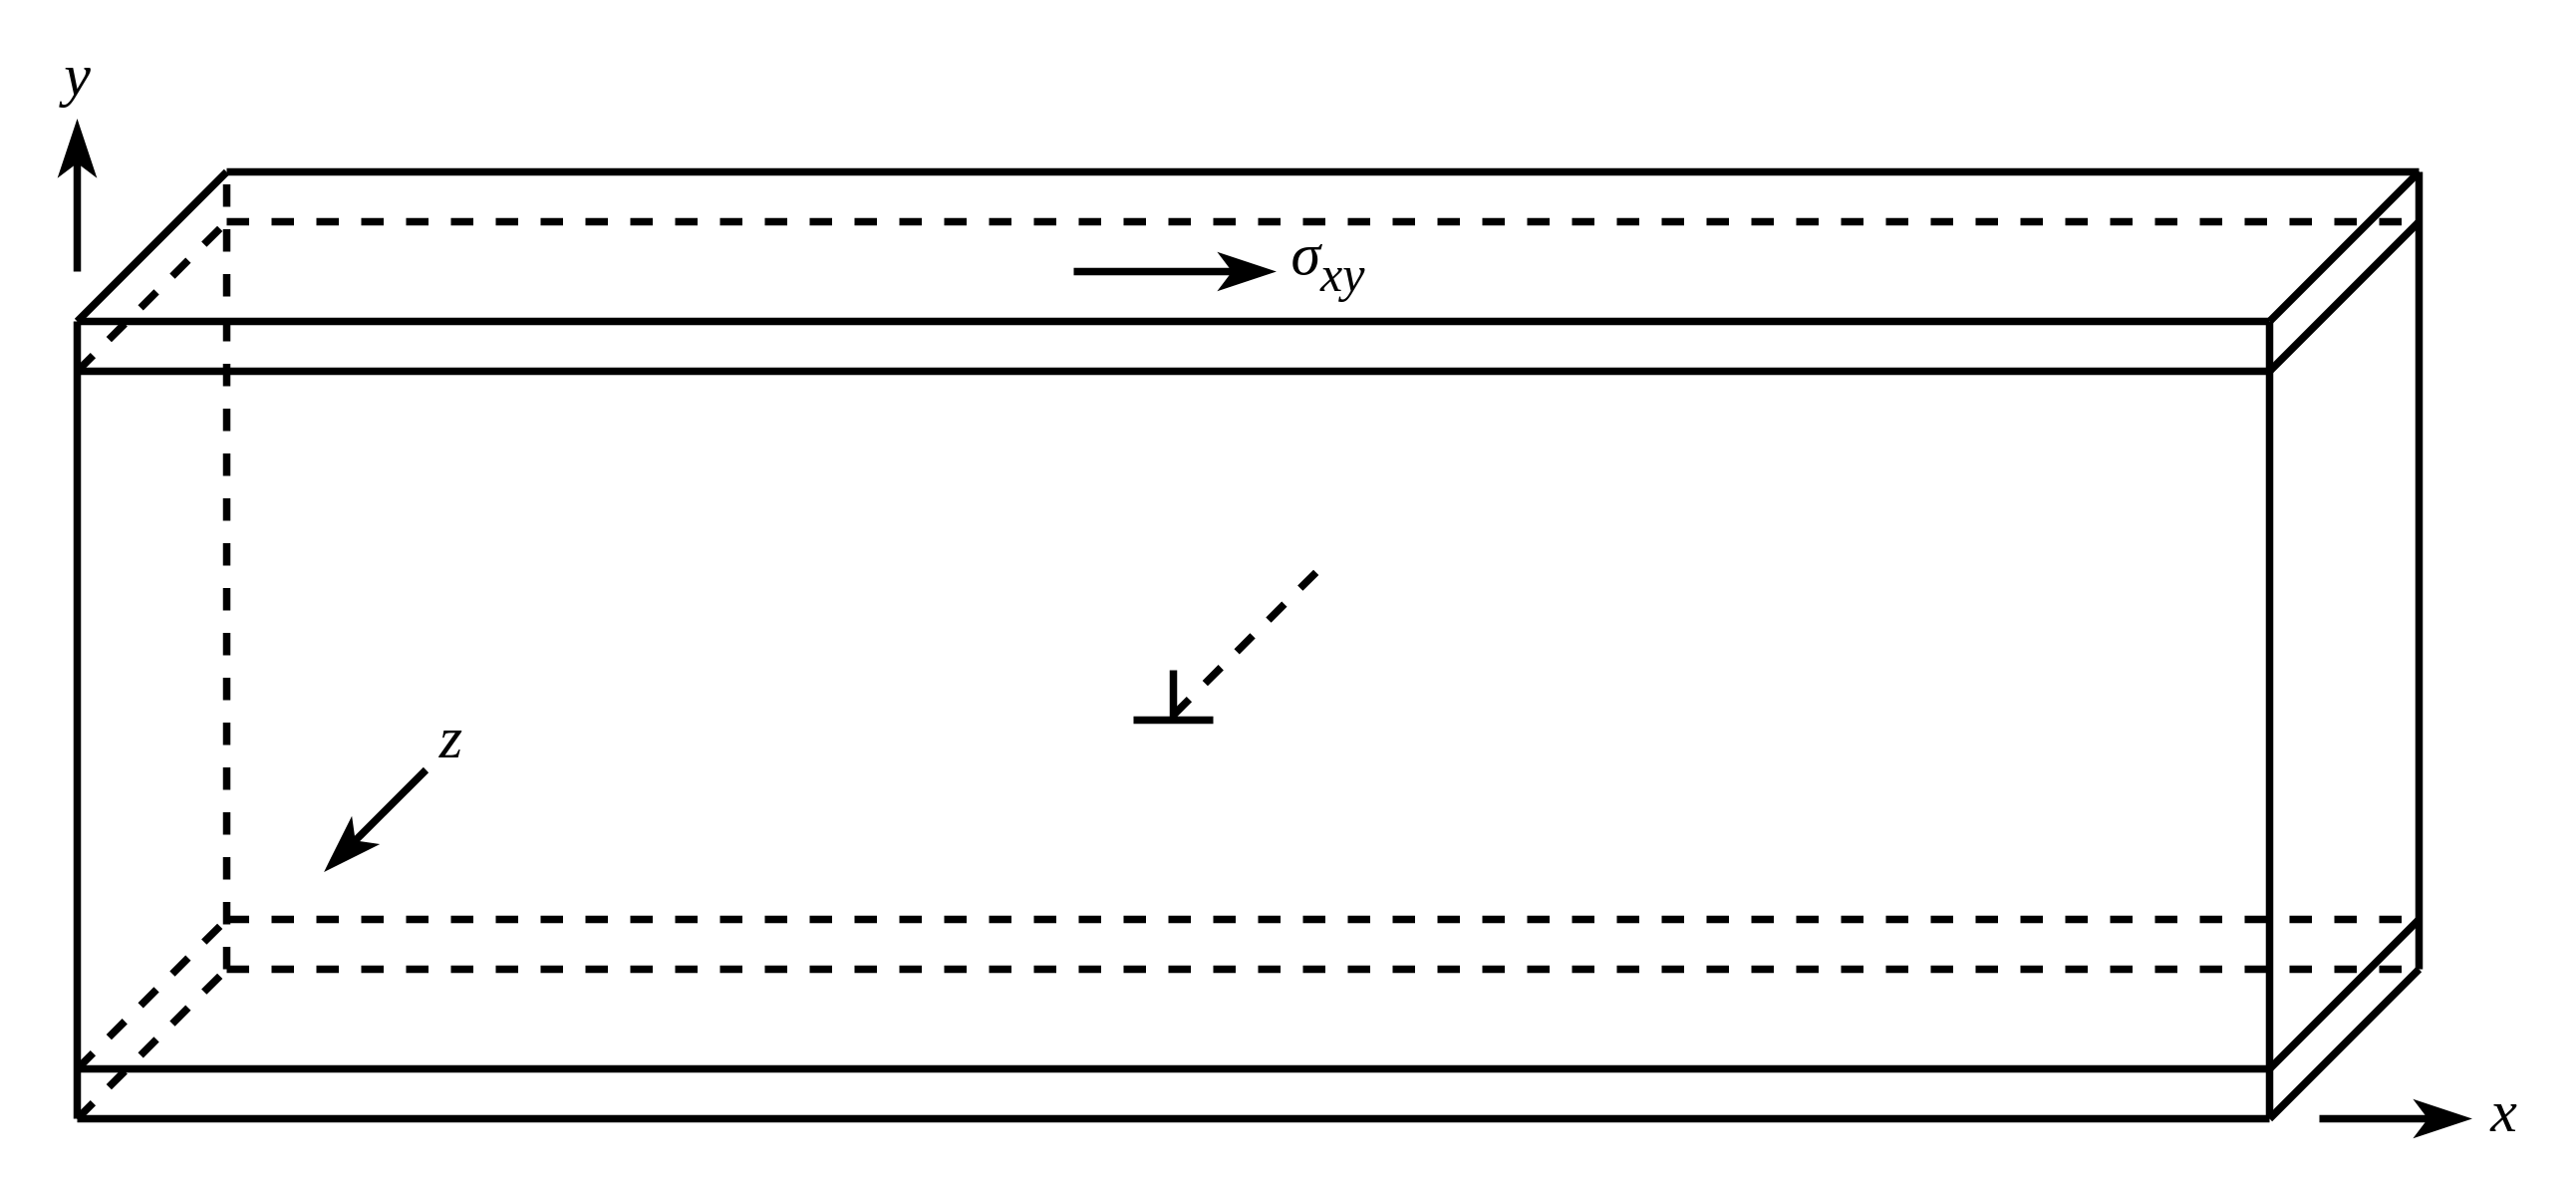
\includegraphics[width=0.48\textwidth]{Qwerty.png}}
\hfill
\subfloat[]{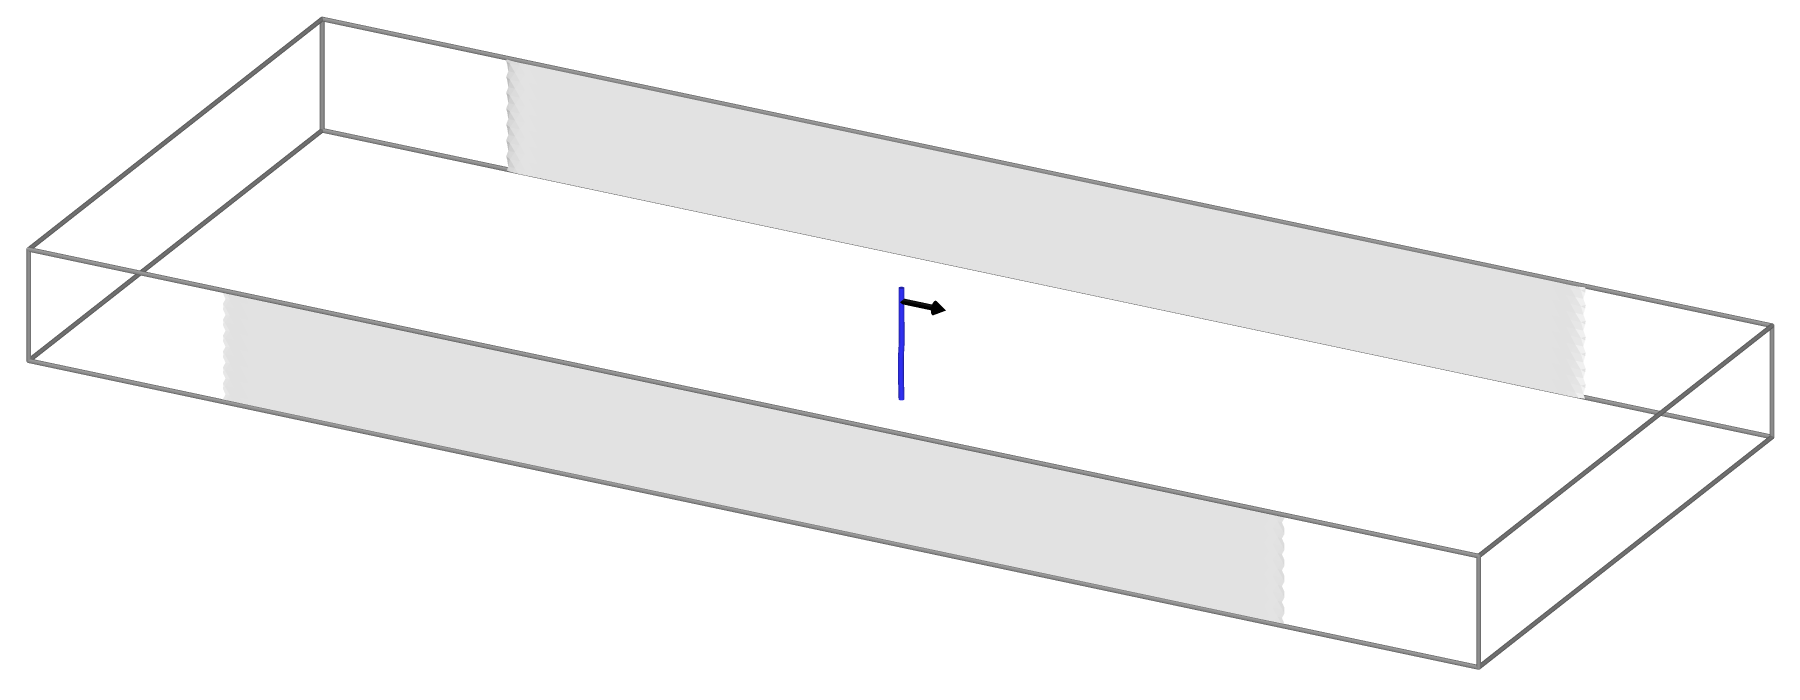
\includegraphics[width=0.48\textwidth]{DislocLine.png}}
}
\caption{(\textbf{a}) \hl{Schematic} %MDPI: Please note that the size of figures will be adjusted appropriately to ensure the clarity and readability of the image. Changes to the position of figures and tables may occur during the production stage. %BB: Understood
 of the supercell constructed to study straight edge dislocations. For~glide along the $\{ 110 \}$ planes, $x = [110]$, $y = [ 1 \Bar{1} 0 ]$, and~$z = [001]$. For~glide along the $\{ 111 \}$ planes, $x= [ \Bar{1} 1 0 ]$, $y = [111]$, and~$z = [ \Bar{1} \Bar{1} 2 ]$. The~top layer on which stress/strain is applied, as well as the fixed bottom layer, is also shown. (\textbf{b}) OVITO visualization of the $\frac{1}{2} [\Bar{1}10] (111)$ edge dislocation and its Burgers vector after equilibration at 1 K. The~free surfaces can be identified from the gray ``defect mesh''. In~(\textbf{a}) the base plane is the $xz$ plane, whereas in (\textbf{b}) the base plane is the $xy$ plane.}
\label{Fig:DislocStructure}
\end{figure}

For the calculation of the Peierls stress at 1 K, the~supercells have approximately the same dimensions: $l_x \approx 550$ \AA, $l_y \approx 200$ \AA, and~$l_z \approx 40$ \AA. Similar simulation setups and supercell dimensions have been used elsewhere~\cite{Osetsky2003, Olmsted2005, Cho2017, Dang2019, Kaloni2023}, where the supercell dimensions along the $x$- and $y$-directions have been chosen to nearly eliminate the effects of the free surfaces and periodic images on the dislocation motion. The~line direction, $l_z$, must be long enough to contain a kink pair, yet not too long so as to contain multiple kinks, which would lead to self-pinning~\cite{Gilbert2011}.

The Kocevski potential was unable to resolve the initial edge dislocation structure of the misfit dislocation into a perfect edge dislocation with a finite Burgers vector. This occurred despite using energy tolerances as low as $10^{-20}$. The~issue likely stems from repulsion between uranium atoms, as~the Kocevski potential cannot stabilize metallic uranium~\cite{AbdulHameed2024}. As~a result, only the Tseplyaev potential was used to study edge dislocations. Both the Kocevski and Tseplyaev potentials could stabilize screw dislocations. However, when simulating the motion of the screw dislocation with the Tseplyaev potential, a~trail of vacancy and interstitial clusters continuously formed during dislocation movement, even at low stresses. In~contrast, the~$\frac{1}{2} [110] ( \Bar{1} 1 0 )$ screw dislocation moved smoothly up to about 1125 MPa under the Kocevski potential. Therefore, the~screw dislocation was studied exclusively with the Kocevski~potential.

The Peierls stress is the applied resolved shear stress that moves a dislocation by at least one Burgers vector without thermal assistance, typically near $T = 0$ K~\cite{Hull2011}. This is usually measured under a condition of constant strain increment~\cite{Puls1976, Osetsky2003}. However, defining strain increments at 0 K is somewhat artificial. Our previous study~\cite{AbdulHameed2024} suggests that the Tseplyaev potential may predict metastable states for UN supercells strained at 0 K. To~avoid these issues, we calculate the Peierls stress at $T = 1$ K using both~potentials.

After static minimization, the~supercell containing a dislocation is equilibrated in the \textit{NVT} ensemble for 50 ps. To~eliminate the impact of thermostat friction, the~thermostat function is simulated with the microcanonical (\textit{NVE}) ensemble coupled to velocity scaling. Once equilibration is complete, velocity scaling is turned off. Shear strain rates $\Dot{\epsilon}_{xy}$ and $\Dot{\epsilon}_{yz}$, both set to $10^{-4}$ s$^{-1}$, are then applied to the top layer of the supercell, containing an edge and screw dislocation, respectively. Osetsky and Bacon~\cite{Osetsky2003} demonstrated that the Peierls stress is independent of strain rate. The~simulation runs for 2 ns, and~the stress on the dislocation is measured by averaging the atomic $\sigma_{xy}$ and $\sigma_{yz}$ stresses for the edge and screw dislocations, respectively, every 10~ps.

The dislocation mobility function is the essential input parameter in any plasticity or dislocation dynamics model~\cite{Kaloni2023}. The~dislocation mobility of UN at 300 K is computed by first scaling the relaxed supercells by the ratio of the 0 K and 300 K lattice parameters after relaxation to correct for thermal expansion~\cite{Cho2017}. Then, the~system is equilibrated at a temperature of 300 K under the \textit{NVE} ensemble coupled to velocity scaling for 50~ps. After~equilibration, a~shear force is applied to the upper layer of the supercell, whose thickness is 0.05 $l_y$. The~simulation is run for 1 ns and the position of the moving dislocation is recorded every 10 ps. The~calculation is repeated using 5 different initial velocity distributions for both dislocation types. The~shear stress for edge dislocations varies between 25 and 2250 MPa, while for screw dislocations, it ranges from 25 to 1200 MPa, with~both cases using a stress increment of 25~MPa.

For all calculations, dislocation motion is tracked using the following methodology: Snapshots of the atomic trajectories of each calculation are processed using OVITO where, for~each snapshot, the~location of the dislocation is identified using the CSP algorithm. Then, the~$x$-coordinate of the dislocation is calculated as the average among the $x$-coordinates of all atoms belonging to the dislocation core. Based on visual inspection and comparison with the DXA applied to the U sublattice, we found that CSP $\geq$ 2 \AA$^2$ exclusively selects the atoms belonging to the dislocation core. A~limitation of this methodology is that it assumes that atoms belonging to the dislocation core only move as a single unit %EE: Please check meaning retained %BB: confirmed
along a single slip plane. For~all calculations in this paper, we confirmed by visual inspection that this is indeed the case. However, this methodology can be extended to study, e.g.,~the cross-slip of screw dislocations by tracking both the $x$- and $y$-coordinates of the dislocation~core.

In general, there exist three regimes for dislocation motion depending on the values of the shear stress (or, equivalently the strain rate) and temperature:

\hl{(\textit{a}) Regime I:} %MDPI: 1. Please check if the following highlighted paragraphs should be revised into mathematical objects, e.g., definition, theorem, lemma, assumption, corollary, proposition, example, etc., or if they should be lists 2. Please confirm if the italic format of the letters a, b and c is necessary and should be retained. %BB: Should be retained as lists. Italicized letters not required, but preferred for formatting clarity.
 Under very low stresses/temperatures, dislocations move via the kink-pair nucleation mechanism, where the dislocations are nearly straight lines, which suggests the existence of only one kink pair at any given time~\cite{Gilbert2011}. Under~these circumstances, the~dislocation motion is thermally activated, and~has an Arrhenius-like dependence on temperature~\cite{Gilbert2011, Starikov2020}:
\begin{equation}
v_\text{I} = v_t \sqrt{s} \ \mathrm{exp} \left[ - \frac{H_0}{2 k_B T} \left(1-s^p\right)^q \right]
\label{Eq:MobI}
\end{equation}
where $v_t$ is the velocity corresponding to the transition from the exponential thermally activated regime (regime I) to the linear phonon drag regime (regime II); $s = \tau/\tau_t$ is the shear stress normalized by the transition stress, $\tau_t$, between~the two regimes; and~$H_0 \left(1-s^p\right)^q$ is the stress-dependent kink-pair nucleation enthalpy, with~$H_0$ being the kink-pair formation energy at zero temperature and zero stress. $H_0$ can be calculated from stress-relaxation measurements or molecular statics~\cite{Ventelon2009, Gilbert2011}. In~this work, however, $H_0$ is treated as a fitting parameter. According to linear elasticity theory, $p=0.5$ and $q=1.25$ for a sinusoidal potential. For~more complex potentials, $p$ and $q$ are treated as fitting parameters, which is our approach in this work, and~they have the following ranges: $0 \leq p \leq 1$ and $1 \leq q \leq 2$.

\hl{(\textit{b}) Regime II:} As the temperature and/or stress are increased, kink-pair nucleation and propagation have comparable rates (i.e., kink-pair nucleation is no longer the rate-limiting step) leading to rough dislocation lines~\cite{Gilbert2011}. Under~these conditions, the~stress is large enough so that there is no thermal barrier to motion, and~the velocity varies linearly with stress~\cite{Dang2019, Olmsted2005}. This viscous drag mainly arises from dislocation interactions with lattice phonons~\cite{Dang2019}. In~this regime, the~velocity takes the form
\begin{equation}
v_\text{II} = \frac{b \tau}{B} + C
\label{Eq:MobII}
\end{equation}
where $b$ is the magnitude of Burgers vector, $B$ is the linear drag coefficient, and~$C$ is an additive constant that has the units of velocity. The~linear dislocation mobility in this regime is calculated as $M = 1/B$.

\hl{(\textit{c}) Regime III:} Under even higher stresses, the~relation between $v$ and $\tau$ becomes nonlinear due to a combination of phonon and radiative damping, with~the velocity asymptotically approaching the transverse sound velocity~\cite{Dang2019}. Radiative damping results from wave emission by moving dislocations and is independent of temperature~\cite{Kresse2004}. In~fracture mechanics, energy dissipation is primarily governed by crack formation rather than radiative damping~\cite{Kresse2004}. As~a result, radiative damping is more relevant to high-velocity deformation scenarios, such as shock loading, than~to cracking-induced failures such as those expected in nuclear fuels under extreme conditions. Therefore, while we identify the transition stress between regimes II and III, $\tau_t'$, regime III is beyond the scope of this study, and~the fitted mobility function is restricted to regimes I and~II.


% In this regime, the relationship between the shear stress and velocity is expressed as
% \begin{equation}
% \tau = \frac{1}{b} \left[ B ( v - v_t ) + D ( v - v_t' )^a \right]
% \end{equation}
% where $D$ is the nonlinear drag coefficient, $v_t'$ is a transition velocity between the linear and nonlinear regimes, and the exponent $a$ is traditionally estimated as $a=1.5$ \cite{Eshelby1956}. 

\section{Results}
%\unskip

\subsection{Deformation~Behavior}
\label{Sec:SS}

The results of the stress--strain computations for single-crystal UN are presented in \cref{Fig:SS}. Additionally, the Young's moduli of UN along the [100] direction, as calculated by \cref{Eq:E100} using experimental and potential-predicted elastic constants as reported in~\cite{AbdulHameed2024,Salleh1986}\hl{,} %MDPI: Reference citations were combined. Please confirm. %BB: confirmed
 respectively, are presented in \cref{Tab:E100}. In~MD stress--strain simulations, a~numerical artifact arises, where the stress continues to oscillate around zero after fracture %MDPI: “Data not shown” should be avoided. Please cite as a reference/Supplementary Materials or please remove this phrase. %BB: phrase has been removed
 due to the interference between the tensile wave and its reflection off the fractured free surface, which results in regions with significant compressive stresses~\cite{Wen2022}. The~stress--strain curves in \cref{Fig:SS} were truncated before displaying these oscillations. Comparing \cref{Fig:SS}a,c to \cref{Tab:E100}, it can be seen that the small-strain $E_{[100]}$ predicted by the Tseplyaev potential (522.7 GPa) is overestimated compared to the large-strain value extracted from the stress--strain curve (410--430 GPa), which is closer to the experimental value (387 GPa), with~the supercell having free surfaces showing the closest agreement. On~the contrary, the~small-strain $E_{[100]}$ predicted by the Kocevski potential (354.1 GPa, \cref{Tab:E100}) is closer to the experimental value than %EE: Please check meaning retained %BB: confirmed
 the large-strain value (300 GPa) as shown in \cref{Fig:SS}b,d. However, both supercells with PBCs and free surfaces have essentially the same Young's modulus. The Young’s moduli of nanocrystalline UN are relevant for bulk UN because Young’s modulus is only slightly affected by structural miniaturization~\cite{Pal2020}.

\begin{figure}[H]
{\captionsetup{position=bottom,justification=centering}
\subfloat[\hl{} %MDPI: We suggest to move explanations of sub-figures to the below figure caption, and retain only labels (a) to (d) here. %BB: Corrected
]{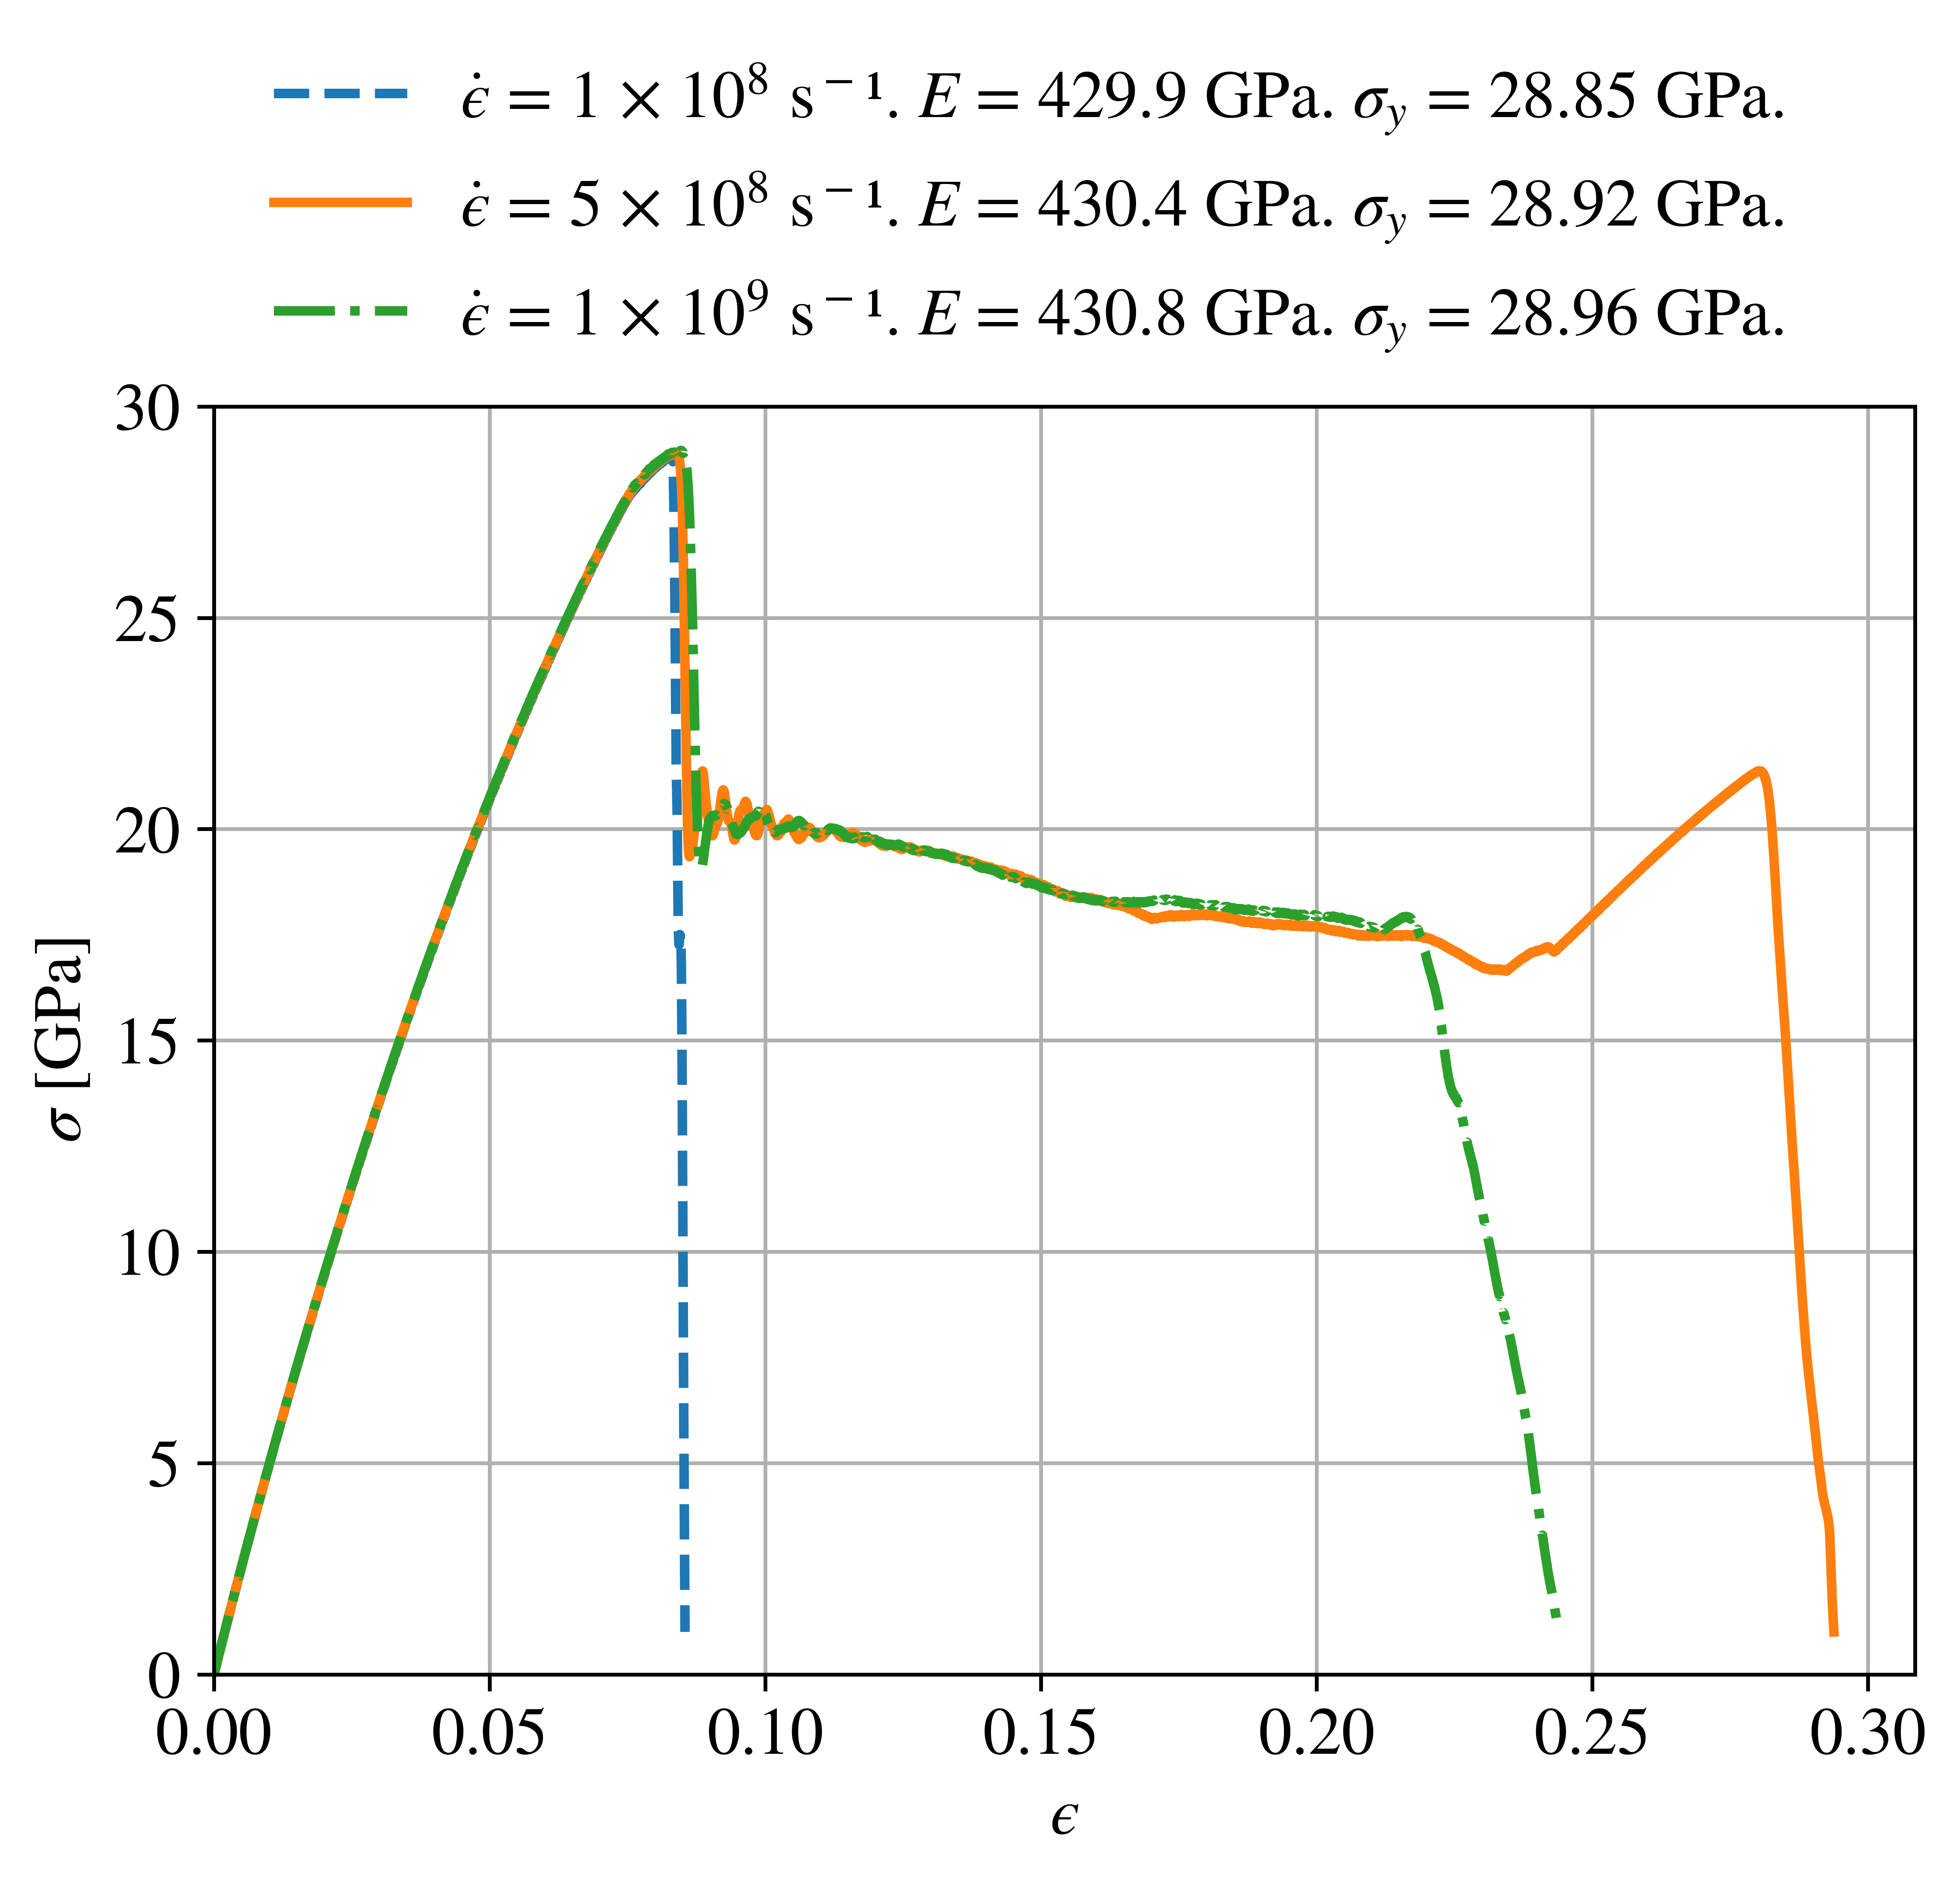
\includegraphics[width=0.48\textwidth]{SS-2-ADP.png}}
\hfill
\subfloat[\hl{}]{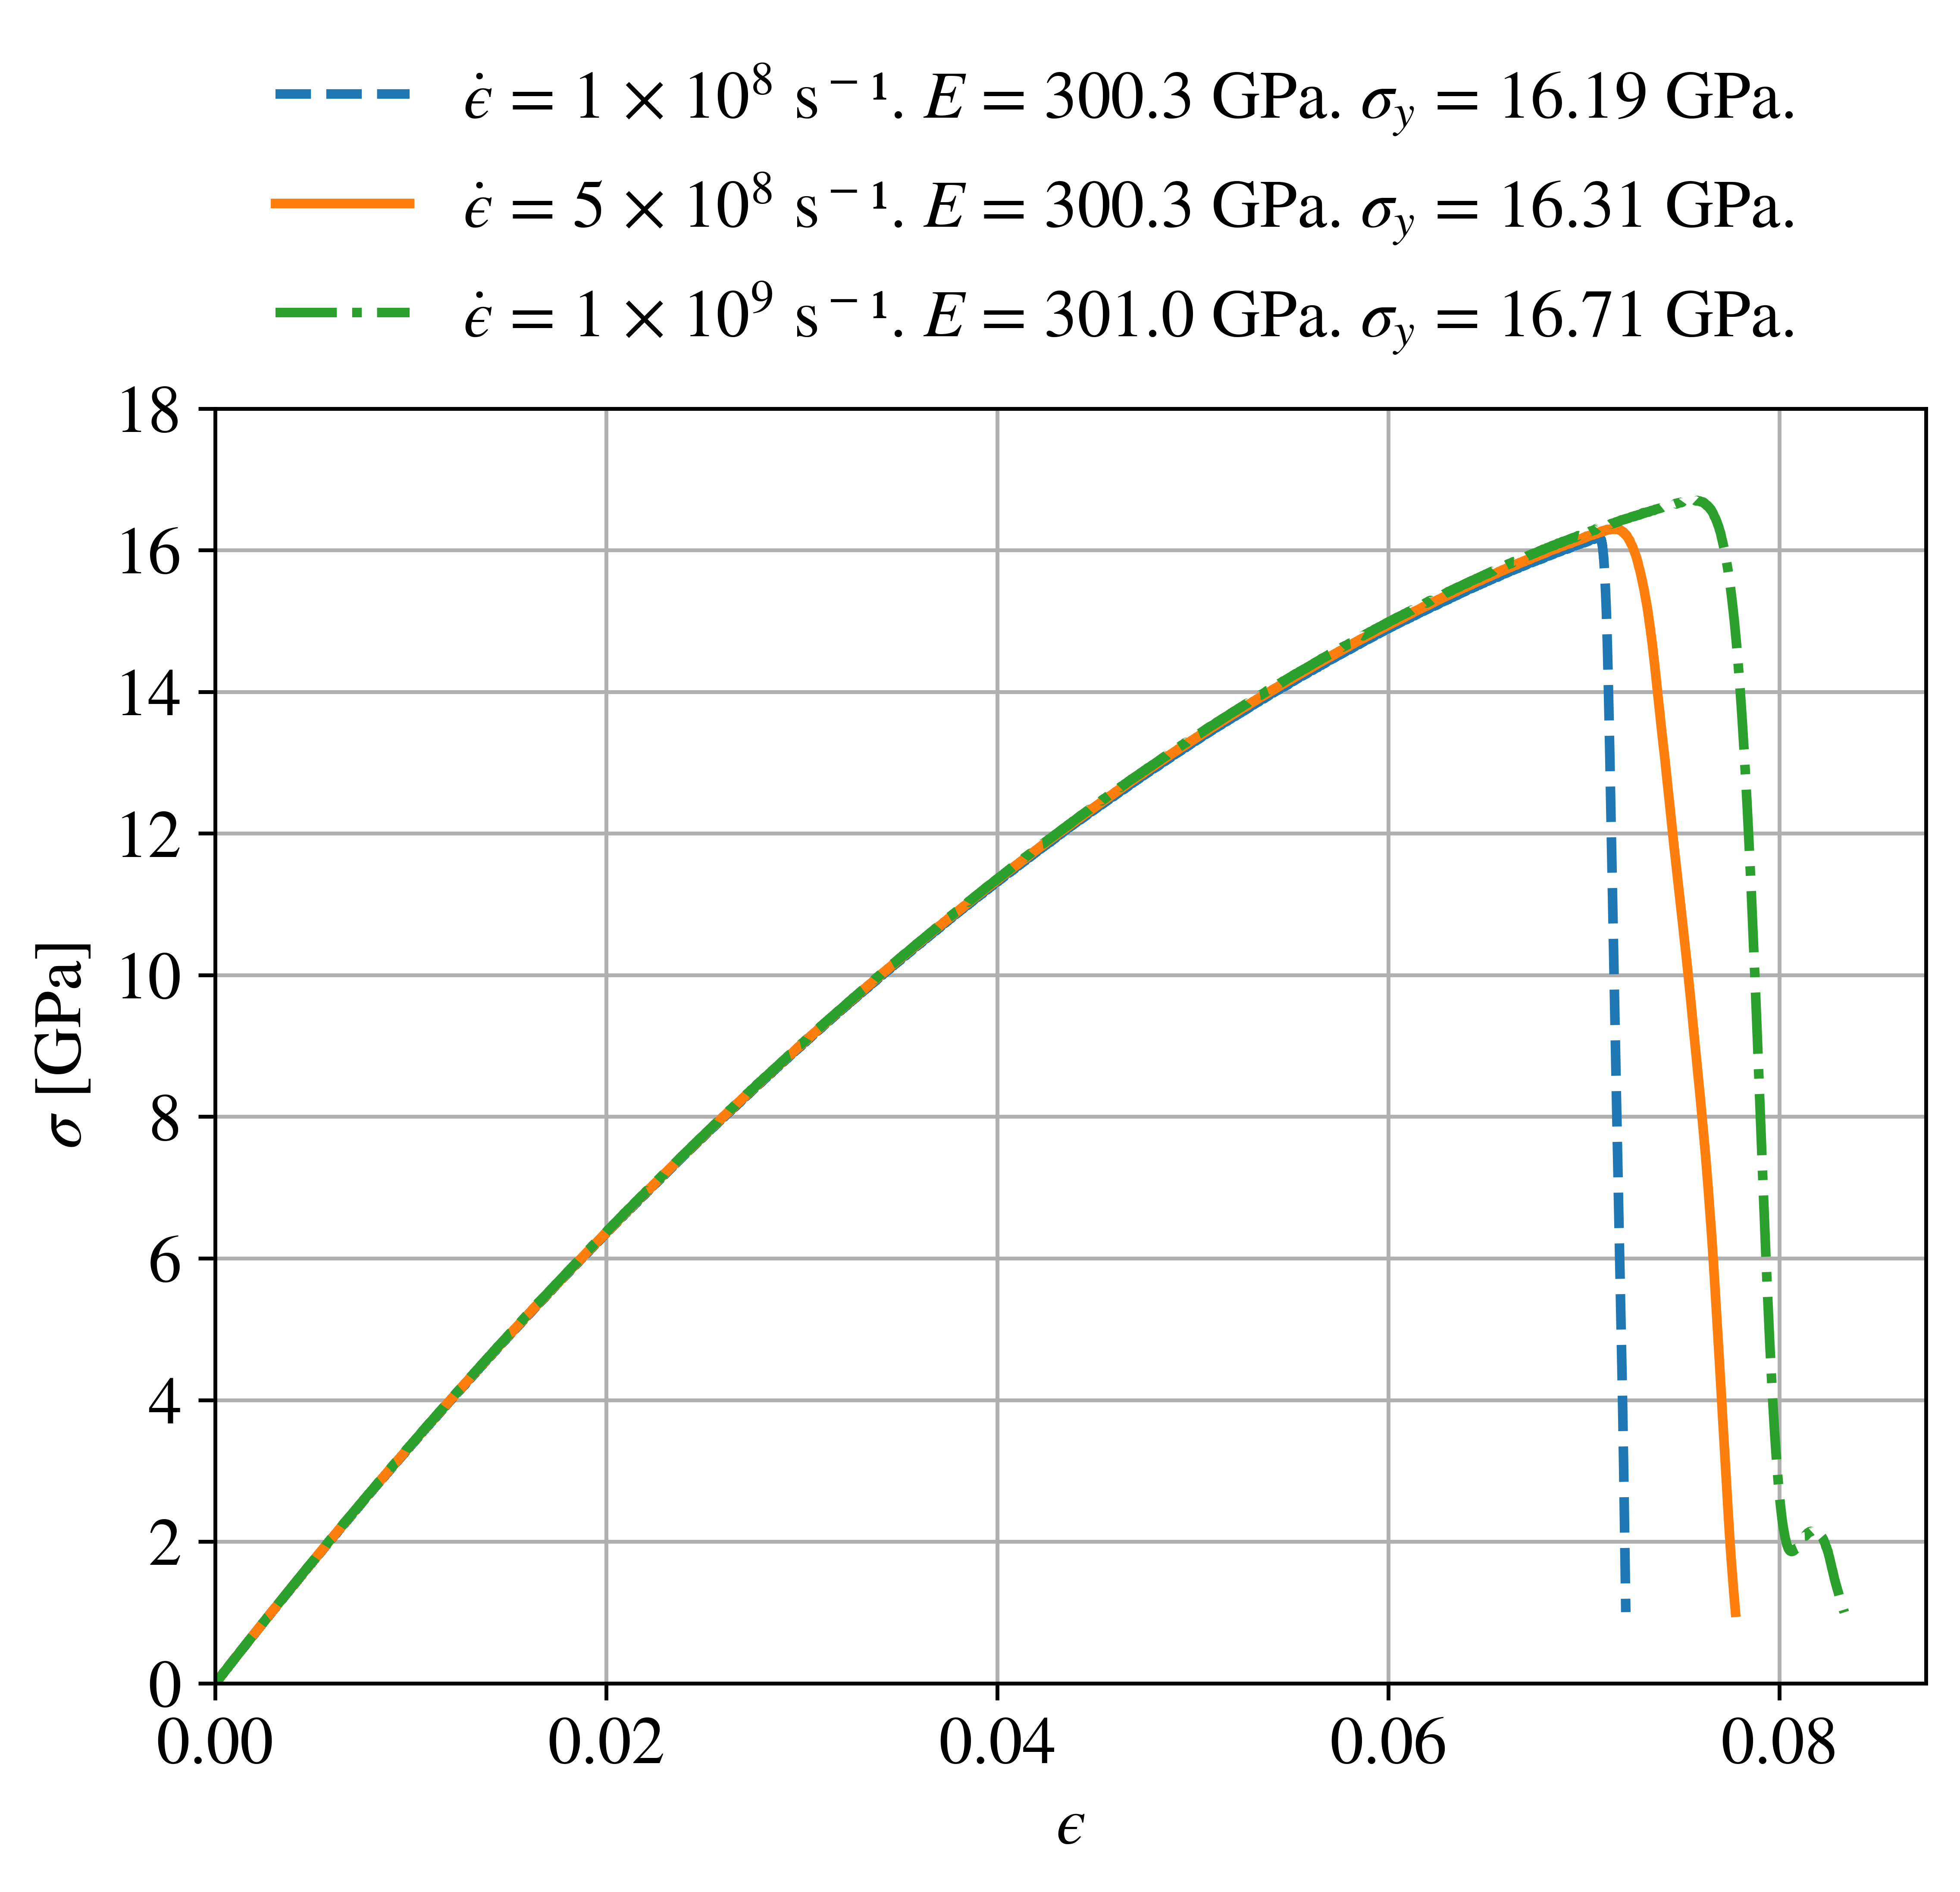
\includegraphics[width=0.48\textwidth]{SS-2-EAM.png}}
\hfill
\subfloat[\hl{}]{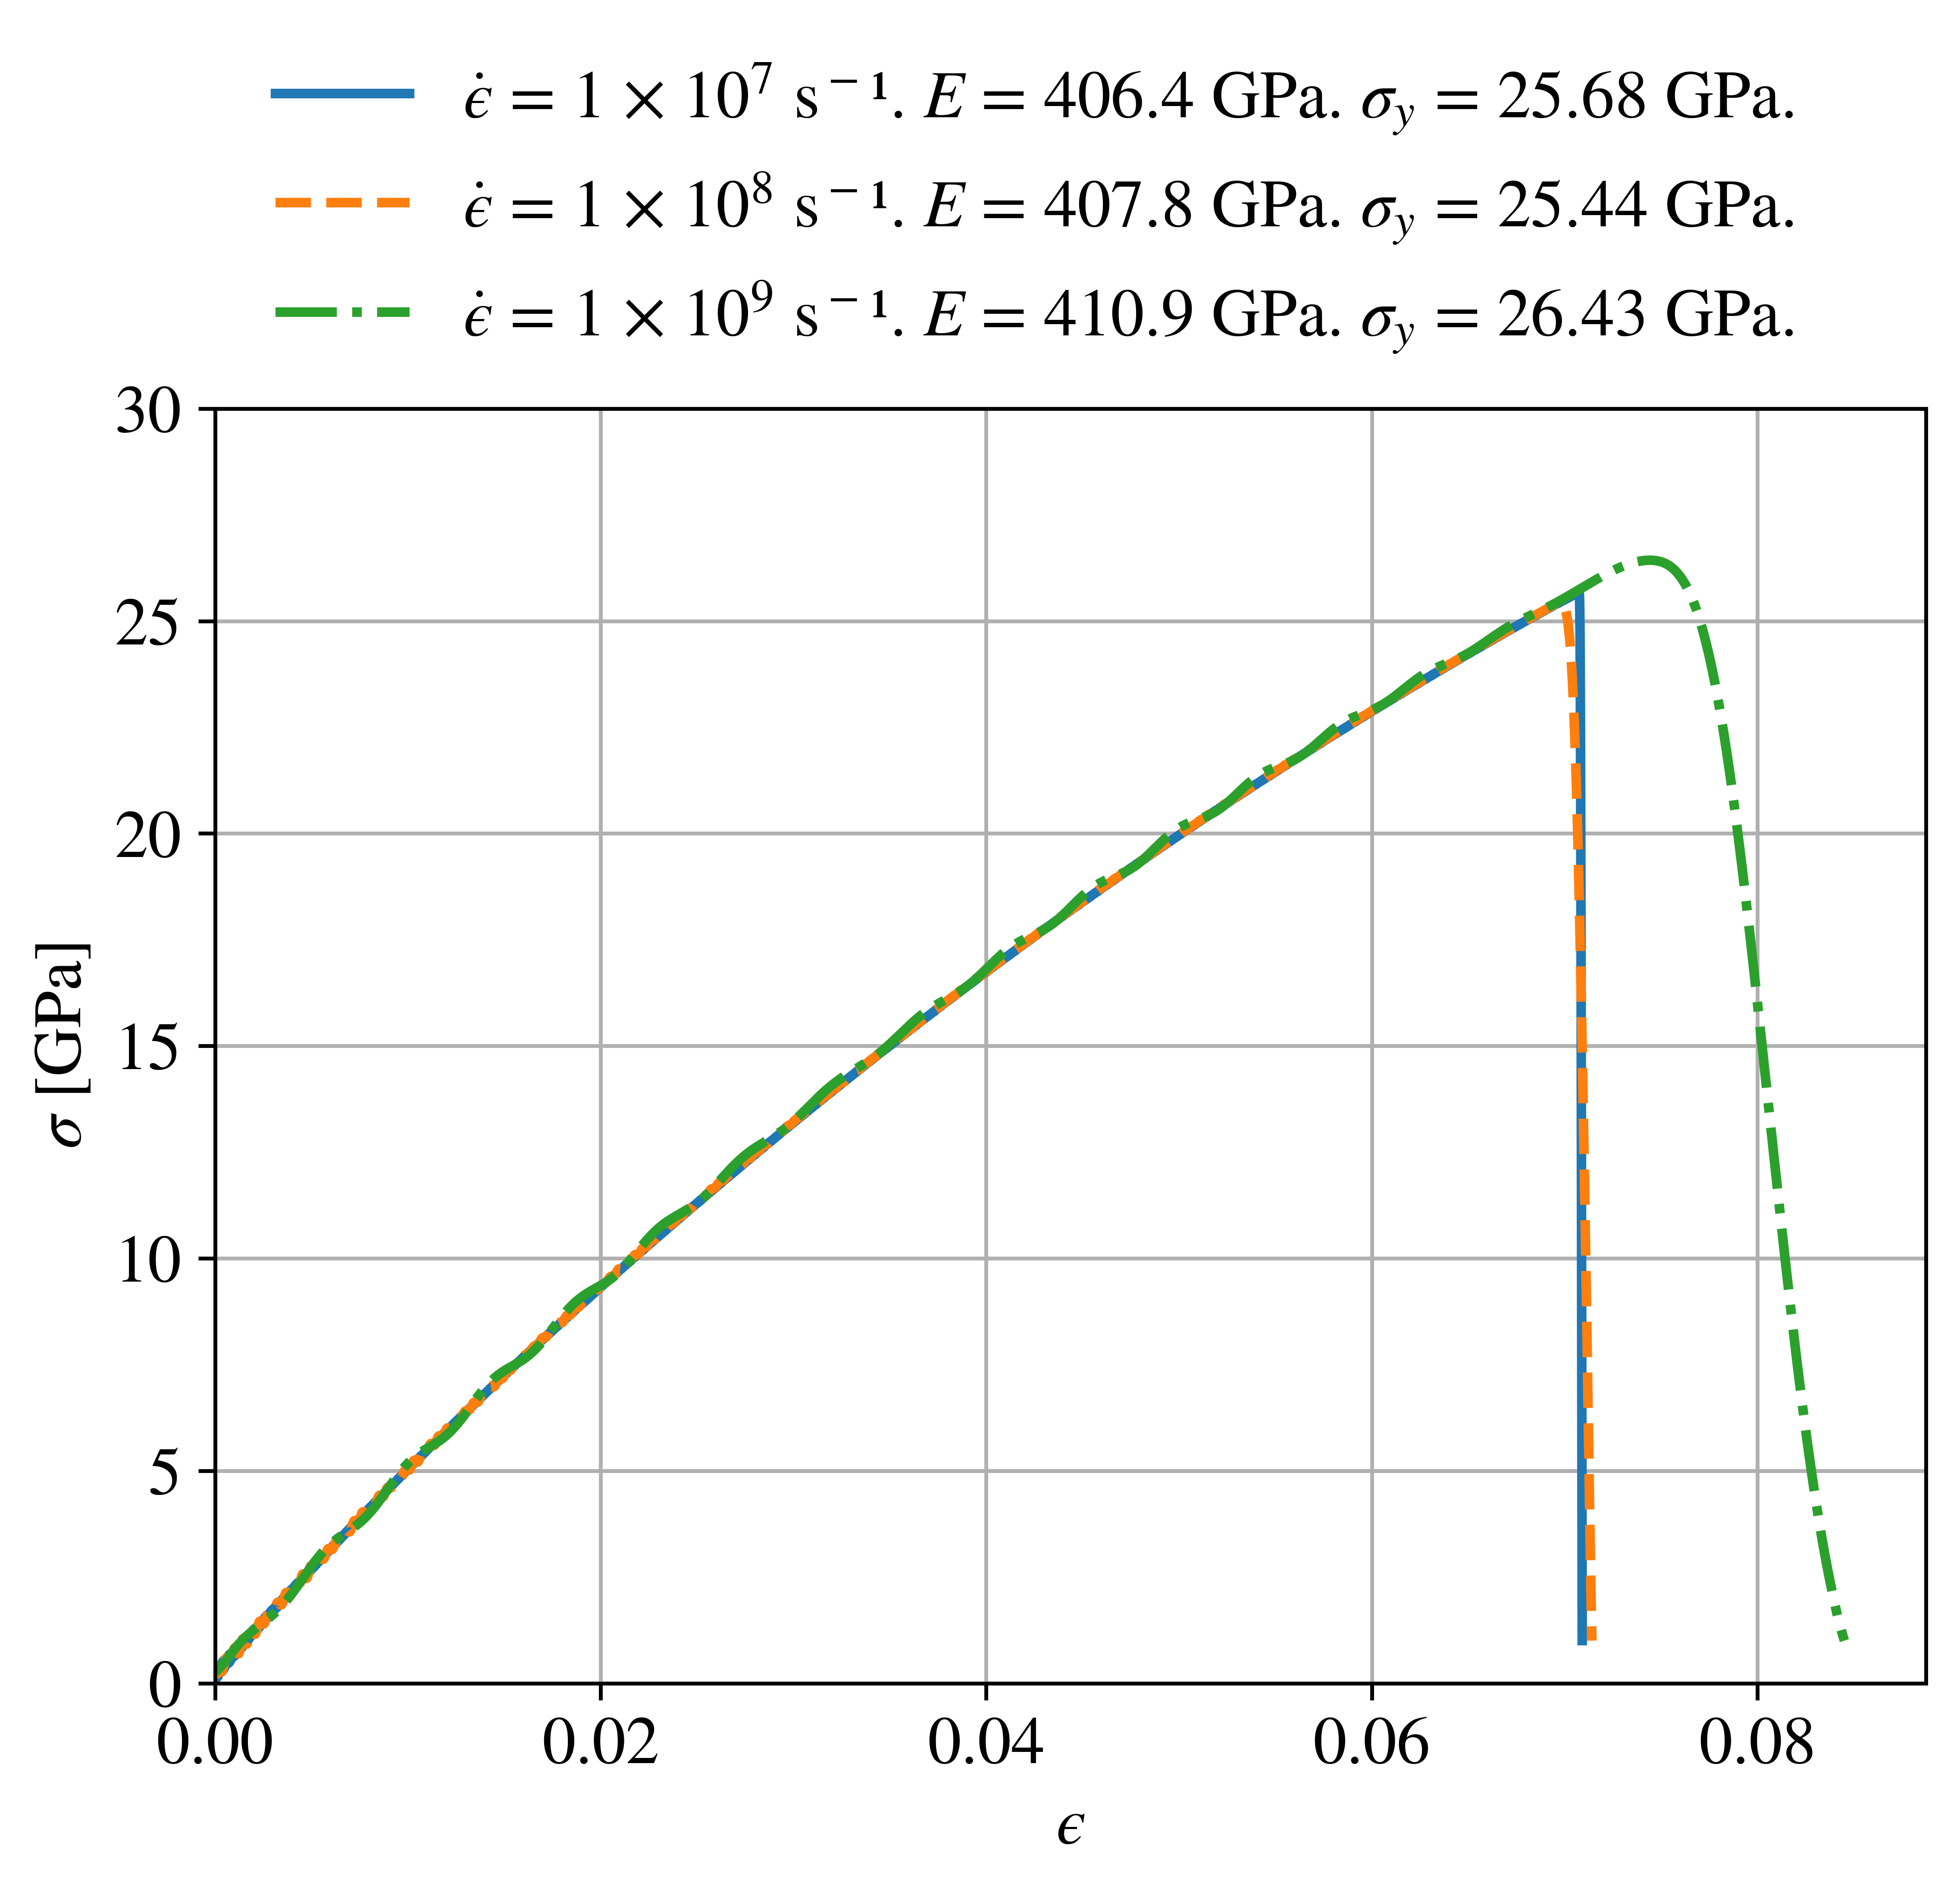
\includegraphics[width=0.48\textwidth]{SS-1-ADP.png}}    
\hfill
\subfloat[\hl{}]{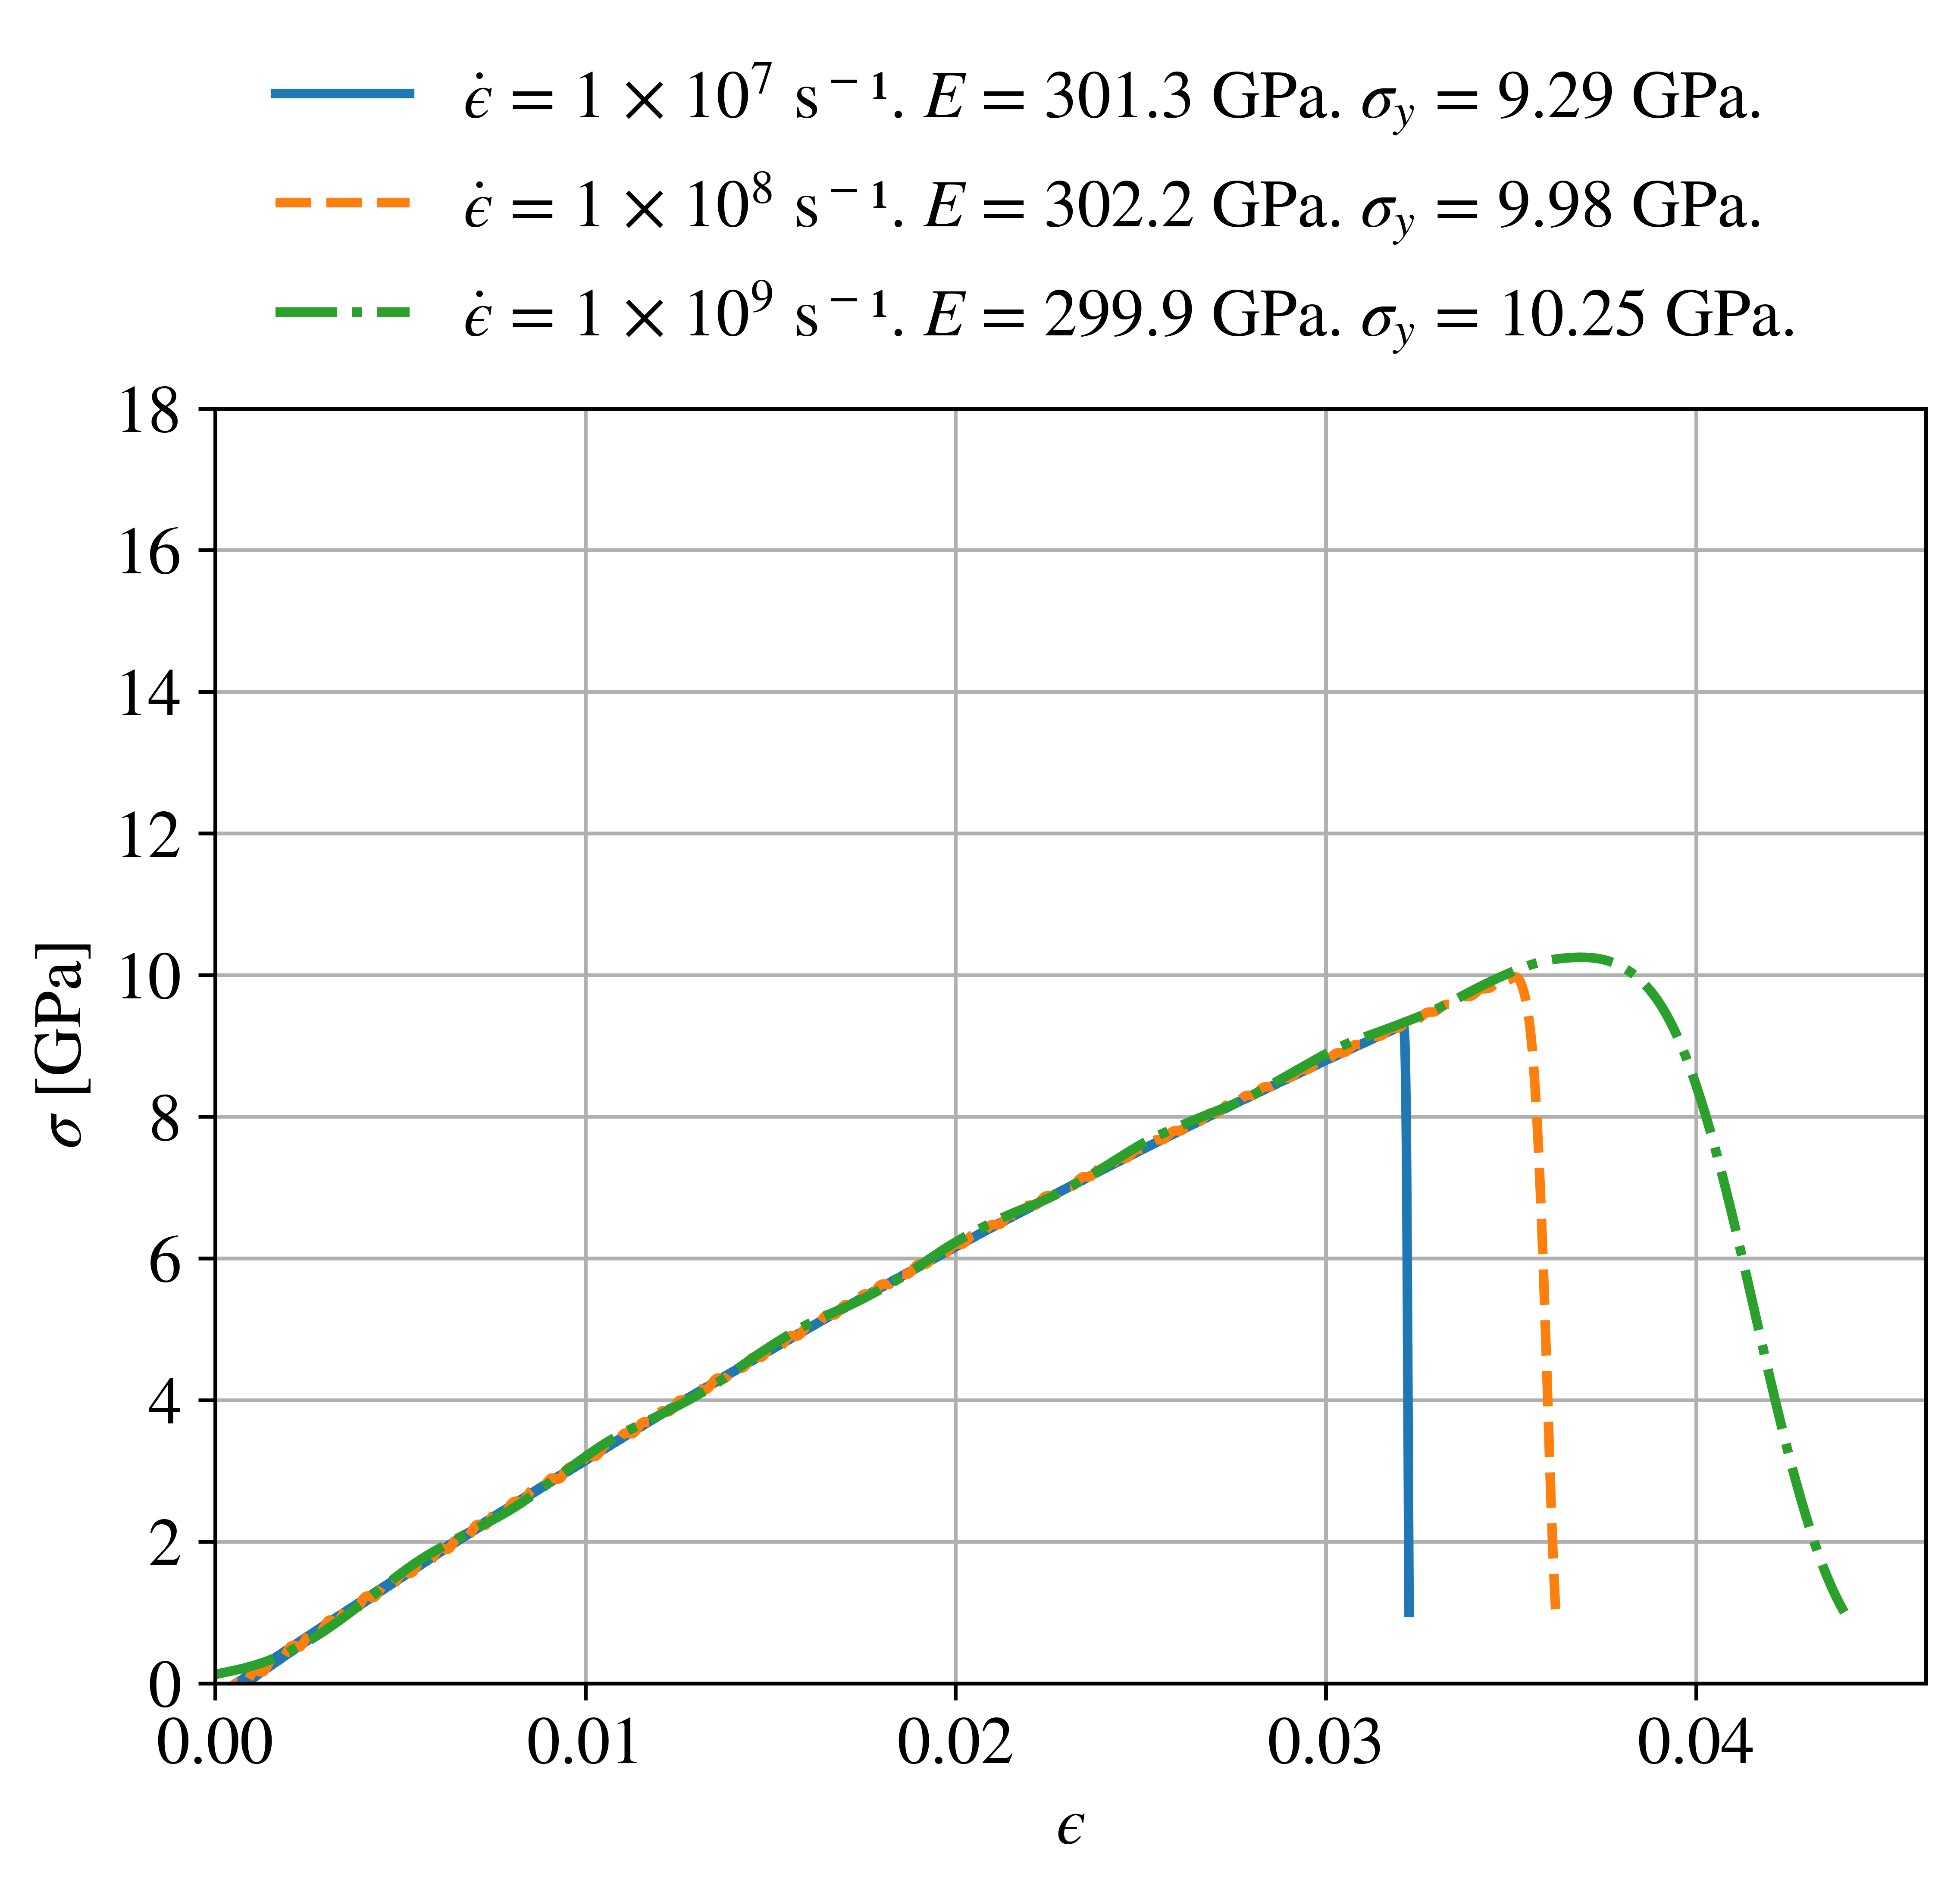
\includegraphics[width=0.48\textwidth]{SS-1-EAM.png}}
}

\caption{(Color online) Stress--strain curves of UN computed at 300 K by (\textbf{a}) the Tseplyaev potential and (\textbf{b}) the Kocevski potential under different strain rates, with PBCs applied in all directions. Stress--strain curves of UN computed at 300 K by (\textbf{c}) the Tseplyaev potential and (\textbf{d}) the Kocevski potential under different strain rates, with PBCs applied only along the loading direction. To~suppress the effect of pressure oscillations on the stress--strain curves for supercells with free surfaces, the~curves calculated by the Tseplyaev and Kocevski potentials have been smoothed by a moving average with windows of 2 and 4 ps, respectively. Note that the $y$-axis range is the same for each potential, whereas the $x$-axis is unique for each~figure.}
\label{Fig:SS}
\end{figure}
%\unskip

\begin{table}[H]
\caption{Small-strain Young's modulus along the [100] direction, $E_{[100]}$ (\cref{Eq:E100}), as~well as the nanoindentation hardness, $H$, of~UN as predicted by both potentials and compared to experimental values at room temperature. The~nanoindentation hardness value of Adachi~et~al. \cite{Adachi2009} represents an average of measurements with loads $< 0.01$ N, where the indentation size effect is not~apparent.}
\newcolumntype{C}{>{\centering\arraybackslash}X}
\begin{tabularx}{\textwidth}{CCCc} 
\toprule
                    & \textbf{Tseplyaev}     & \textbf{Kocevski}  & \textbf{Experimental} \\
\midrule
$E_{[100]}$ [GPa]   & 522.7         & 354.1     & 387.0~\cite{Salleh1986}   \\
$H$ [GPa]           & 25.38         & 9.28      & 7.8 $\pm$ 0.2~\cite{Frazer2021}, 9.7 $\pm$ 0.4~\cite{Adachi2009}    \\
\bottomrule
\end{tabularx}
\label{Tab:E100}
\end{table}

% The velocity of the deformation can be estimated from:
% \begin{equation}
% v = \Dot{\epsilon} l_x
% \end{equation}
% where $l_x$ is the dimension of the supercell along the loading/tensile direction.

The yield stresses predicted by the Tseplyaev potential for nanocrystalline UN strain under PBCs (\cref{Fig:SS}a) are larger than those %EE: Please check meaning retained %BB: confirmed
predicted by the Kocevski potential (\cref{Fig:SS}b) by more than a factor of 2. The ultrahigh yield stresses in the range of about 30 GPa predicted by the Tseplyaev potential are characteristic of purely covalent nanomaterials like Si and SiC~\cite{Ivashchenko2007}, which is not the case for UN, whose bonding environment has both ionic and covalent character~\cite{Kuksin2016}. At~all strain rates, the~Kocevski potential predicts brittle fracture for nanocrystalline UN (\cref{Fig:SS}b). Interestingly, however, for~strain rates of $5 \times 10^{8}$ and \mbox{$10^{9}$ s$^{-1}$,} the~Tseplyaev potential predicts sustainable plastic deformation by dislocation motion along the $\{ 111 \}$ planes (\cref{Fig:Slip}). The~stress--strain curves show signs of stress relaxation after yielding and multiple slip planes develop along the entire length of the specimen. The~drop in the stress--strain curve after yielding is attributed to the development of dislocation planes~\cite{Pal2020}. Necking occurs as a result of the branching of secondary dislocation planes from a primary dislocation plane~\cite{Pal2020}, as can be observed in \cref{Fig:Slip}.

\begin{figure}[H]
    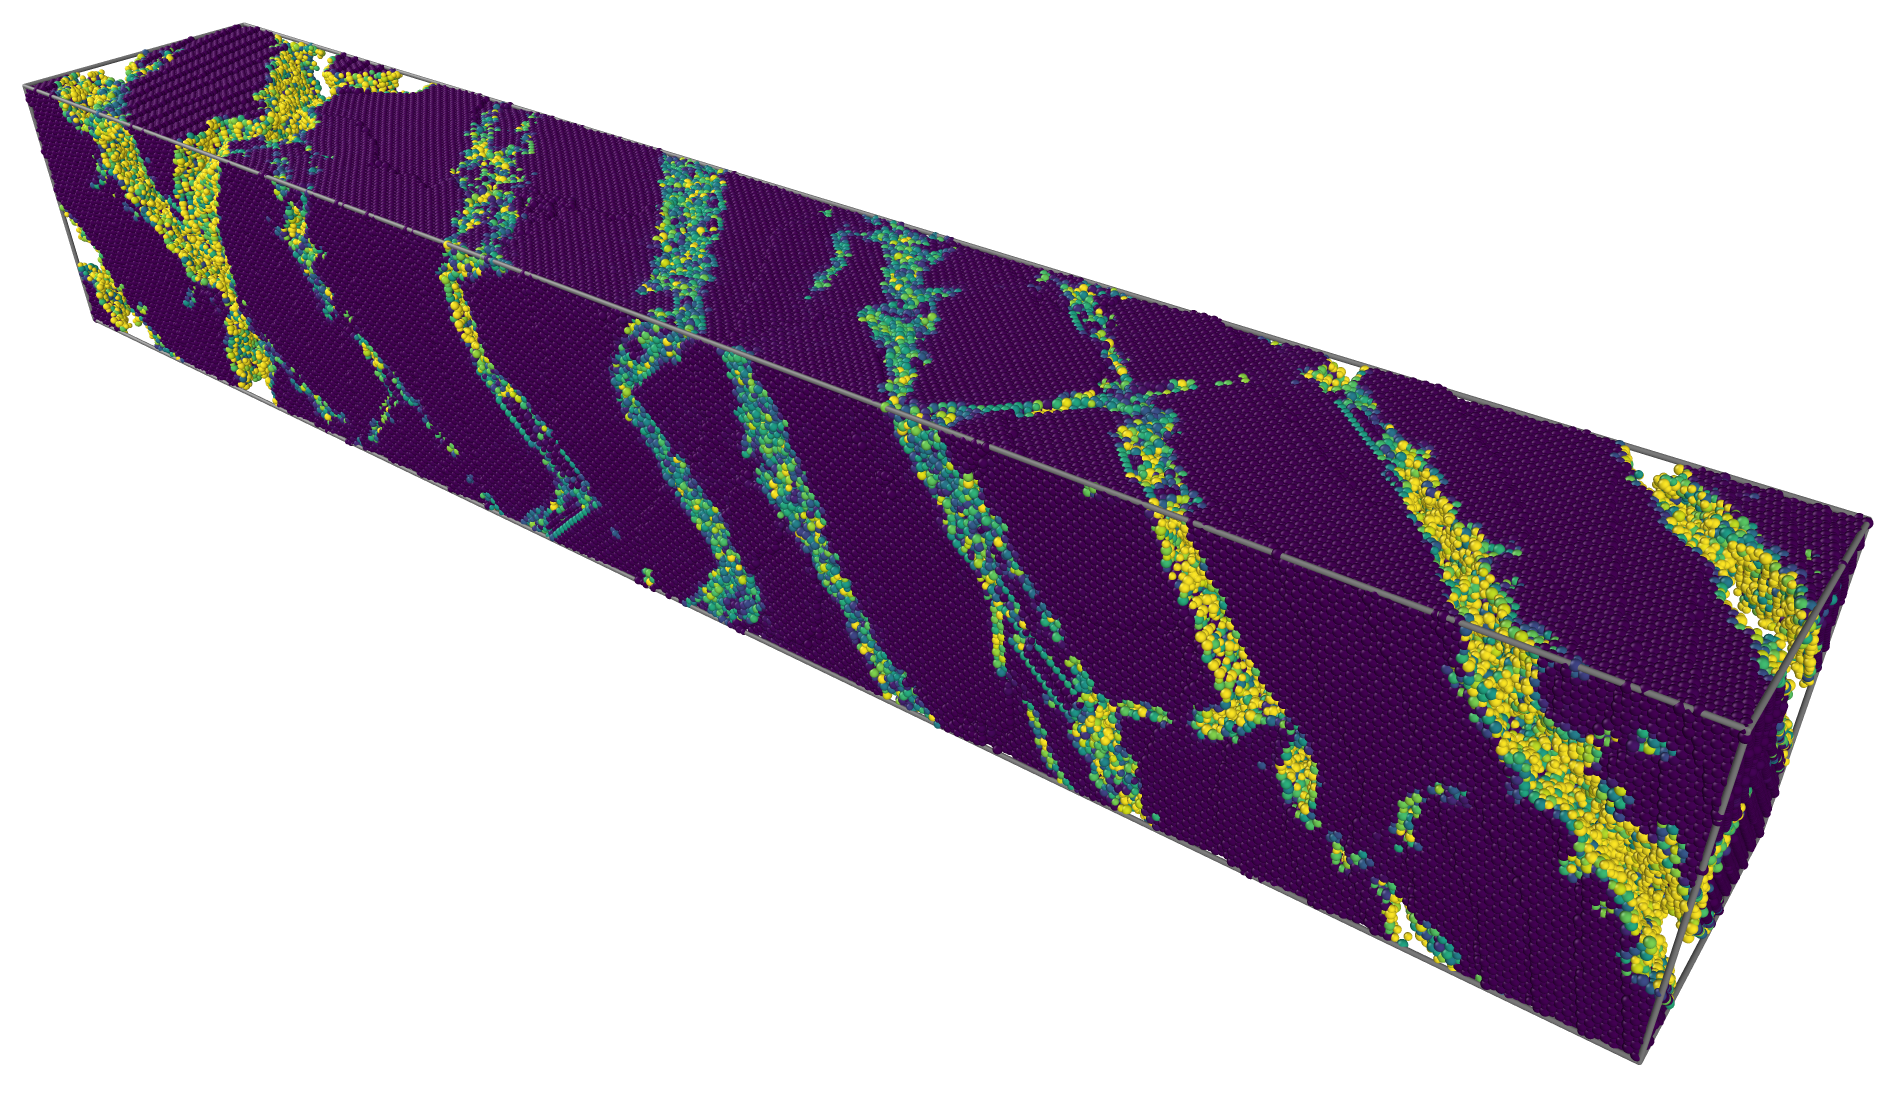
\includegraphics[width=0.70\textwidth]{SlipADP1e9.png}
    \caption{\hl{(Color online)} %MDPI: Please provide an explanation of each color if necessary. %BB: color explanation included in the caption
 $\{ 111 \}$ slip planes generated in the $150 \times 30 \times 30$ supercell when strained at 300 K and a strain rate of $10^{9}$ s$^{-1}$ under PBCs, as modeled by the Tseplyaev potential. Atoms have been colored in OVITO according to their CSP, where dark purple atoms have zero CSP and yellow atoms have high CSP. For~better visibility, the~maximum CSP has been set to 20 \AA$^2$. Similar slip planes have been observed at a strain rate of $5 \times 10^{8}$ s$^{-1}$.}
    \label{Fig:Slip}
\end{figure}

The finding that UN slips primarily along the $\{111\}$ planes is interesting because it contradicts the principal slip system reported by Sole and van der Walt for UN, which is $\{110\}$ \cite{Sole1968}. $\{110\}$ planes are the preferred slip system for purely ionic \mbox{crystals~\cite{VanDerWalt1967, Hull2011}.} For~crystals with a mixed ionic--covalent bonding environment (as in the case of UN), slip might principally occur along other planes, e.g.,~$\{111\}$ and $\{100\}$ \cite{VanDerWalt1967, Yadav2014}. More interestingly, the~primary slip planes in uranium monocarbide (UC) and titanium carbide, two compounds closely related to UN, have been reported to be $\{111\}$ \cite{Sole1968, Vasudevamurthy2022}, which raises questions about the physical reason for this~discrepancy.

Van der Walt and Sole attempted to explain the different slip systems of UN and UC in another study~\cite{VanDerWalt1967} by formulating a hard-sphere model for MX compounds with the NaCl crystal structure, in which the radius ratio, i.e.,~$R_\text{X}/R_\text{M}$, affected the saddle point configuration of the $\frac{1}{2}\langle110\rangle$ dislocation during its motion. Based on this model, three cases arose: (\textit{a}) crystals with $R_\text{X}/R_\text{M} \approx 0.414$ slip on $\{110\}$; (\textit{b}) for $0.414 < R_\text{X}/R_\text{M} < 0.633$, slip is on $\{111\}$; and (\textit{c}) for $R_\text{X}/R_\text{M} > 0.633$, slip occurs on $\{100\}$. They further assumed that $R_\text{M}$ was equal to the metallic radius, and~$R_\text{X} = a_\text{MX}/2 - R_\text{M}$, where $a_\text{MX}$ is the lattice parameter of the compound MX. Based on this definition, the~authors found that for UN, $R_\text{X}/R_\text{M} = 0.41$, which predicts slip on $\{110\}$, whereas for UC, $R_\text{X}/R_\text{M} = 0.43$, which predicts slip on $\{111\}$. However, the~choice of the metallic radius, $R_\text{M}$, was rather~arbitrary.

To confirm that we are observing dislocations along slip planes, the~DXA was applied to the supercell immediately after fracture, and~it was found that perfect dislocations (of both edge and screw characters) with $\mathbf{b} = \frac{1}{2} \langle 110 \rangle$ (which is the usual Burgers vector in ionic crystals~\cite{Hull2011}) reside along the planes with a high CSP. We also observed several Shockley partials with a Burgers vector $\frac{1}{6}\langle112\rangle$ along the slip planes. Historically, the~existence of Shockley partials in ionic crystals has been the source of much debate in the \mbox{literature~\cite{Smoluchowski1966, Haasen1985}.} Based on geometrical and energetic arguments, it was shown that for an ionic MX compound that has the NaCl crystal structure and slips on the $\{111\}$ planes, only perfect dislocations can exist, because the presence of the smaller X atoms prevents the occurrence of Shockley partials~\cite{VanDerWalt1967}. Thus, the~observed Shockley partials may be either an artifact of the dislocation analysis algorithm or an intermediate metastable state predicted by the Tseplyaev potential. Another possibility is that the Tspelyaev potential overestimates the covalency of UN. In~\cref{Fig:Slip}, we can also see signs of cross-slip along planes of the $\{111\}$ family. This is expected, as~cross-slip of screw dislocations with $\mathbf{b} = \frac{1}{2}\langle110\rangle$ can occur only by glide on planes other than $\{110\}$, as~only one $\langle110\rangle$ direction lies in a given $\{110\}$ plane~\cite{Hull2011}.

It should be pointed out that at a strain rate of $10^{8}$ s$^{-1}$, the~Tseplyaev potential shows no sign of dislocation formation or slip. The~reason for this is that the formation of dislocations in a defect-free structure requires high energy deposition rates to form and move dislocations of large Burgers vectors~\cite{Desai2008, Pal2020}, which are only attainable at high strain rates. It should be emphasized that no dislocation nucleation is observed for the Kocevski potential, regardless of strain~rate.

As expected, supercells with free surfaces (\cref{Fig:SS}c,d) show no signs of plastic behavior~\cite{Ivashchenko2007}. Based on these curves, we have calculated estimates of the nanoindentation hardness that are outlined in \cref{Tab:E100}. To~obtain these values, the~maximum stresses of the stress--strain curves for supercells with free surfaces strained at rates of $10^7$, $10^8$, and~$10^9$ s$^{-1}$ have been linearly extrapolated to a zero strain rate. It can be seen that the nanoindentation hardness estimated by the Kocevski potential is very close to the experimental value calculated by Frazer~et~al. \cite{Frazer2021} at 300 K, whereas that estimated by the Tspelyaev potential is overestimated by more than a factor of 3. It should be emphasized that this method is based on an observed empirical correlation between the yield stress of the supercell with free surfaces and the nanoindentation hardness, despite the deformation mechanisms in both being different. That is, nanoindentation experiments are associated with the formation of a plastic zone (with many dislocations) below the indent~\cite{Adachi2009}, whereas the brittle fracture of the supercells with free surfaces shows no signs of plasticity. This correlation is justified because, although~UN fails through plastic deformation, its brittle fracture provides insight into the yield stress of the material~\cite{Taylor2008} (which is often correlated with the hardness~\cite{Meyers2009}), at~which point the elastic limit is reached and plastic deformation~initiates.

The nanoindentation hardness of UN could not be measured by Frazer~et~al. \cite{Frazer2021} at $T > 473$ K due to the formation of an oxidation layer on the surfaces of UN samples at higher temperatures. In~MD simulations, the~formation of an oxidation layer is not an issue. Thus, this method can be used to estimate the nanoindentation hardness at higher temperatures provided we demonstrate that the empirical potential accurately predicts the mechanical behavior at the relevant~temperatures.

\subsection{Dislocation~Motion}
\label{Sec:DislocMotion}

\subsubsection{Edge~Dislocations}

A schematic of the supercell constructed to study edge dislocations as well as the OVITO visualization of the $\frac{1}{2} \langle 110 \rangle \{111\}$ edge dislocation and its Burgers vector after equilibration at 1 K are shown in \cref{Fig:DislocStructure}. It is noted that the Kocevski potential could not stabilize edge dislocations, and only the Tseplyaev potential is used for their simulation. The~gray ``defect mesh'' in \cref{Fig:DislocStructure}b extends over about two-thirds of $l_x$, as~the dislocation's presence is not sensed far from the dislocation line. The~defect mesh is an OVITO term for crystal regions where the atomic arrangement deviates from that of a perfect crystal. This implies that the chosen supercell dimensions are indeed large enough to have a strain-free state, where PBCs are applied along the slip direction. A~supercell similar to \cref{Fig:DislocStructure} was constructed for the screw dislocation, and~the same observation about the defect mesh applies to it. We note that after 0 K minimization, the~$\frac{1}{2} \langle 110 \rangle \{111\}$ edge dislocation splits into two Shockley partials with $\mathbf{b} = \frac{1}{6} \langle 112 \rangle$. However, when the supercell is equilibrated at 1 K, the~Shockley partials transform back to a perfect edge dislocation. Thus, the~Tseplyaev potential predicts Shockley partials to exist only as a metastable state in UN. % Historically, there has been substantial debate on the existence of partial dislocations and stacking faults in ionic crystals~\cite{Smoluchowski1966, Puls1976, Puls1980, Haasen1985}.


The displacement and stress of the $\frac{1}{2} \langle 110 \rangle$ edge dislocation as a function of time is shown in \cref{Fig:Disloc}. We can observe that the Peierls stress of the $\frac{1}{2} \langle 110 \rangle$ edge dislocation along the $\{ 111 \}$ plane is 2.98 GPa, whereas those for the $\{ 110 \}$ and $\{ 112 \}$ planes are 7.65~GPa and 8.82 GPa, respectively. This confirms that $\{ 111 \}$ is the principal slip plane in UN, as predicted by the Tseplyaev potential, because it requires the lowest stress for slip. It is also found that  $\{ 110 \}$ is predicted to be the second preferable slip plane. A~Peierls stress of 2.98 GPa is on the order of 10$^{-2}$ $G$, $G$$\sim$100 GPa being the shear modulus of UN as predicted by the Tseplyaev potential~\cite{AbdulHameed2024}. This is the same order of magnitude of the Peierls stresses for purely covalent materials~\cite{Hull2011}, which confirms our conclusion that the Tspelyaev potential very likely overestimates the covalency of the UN system. For~purely ionic crystals like LiF and NaCl, the~experimental values of the Peierls stress are $1.6 \times 10^{-4}~G$ and~$5.0 \times 10^{-4}~G$, respectively~\cite{Liu2012}.

\begin{figure}[H]
\centering
{\captionsetup{position=bottom,justification=centering}
\subfloat[]{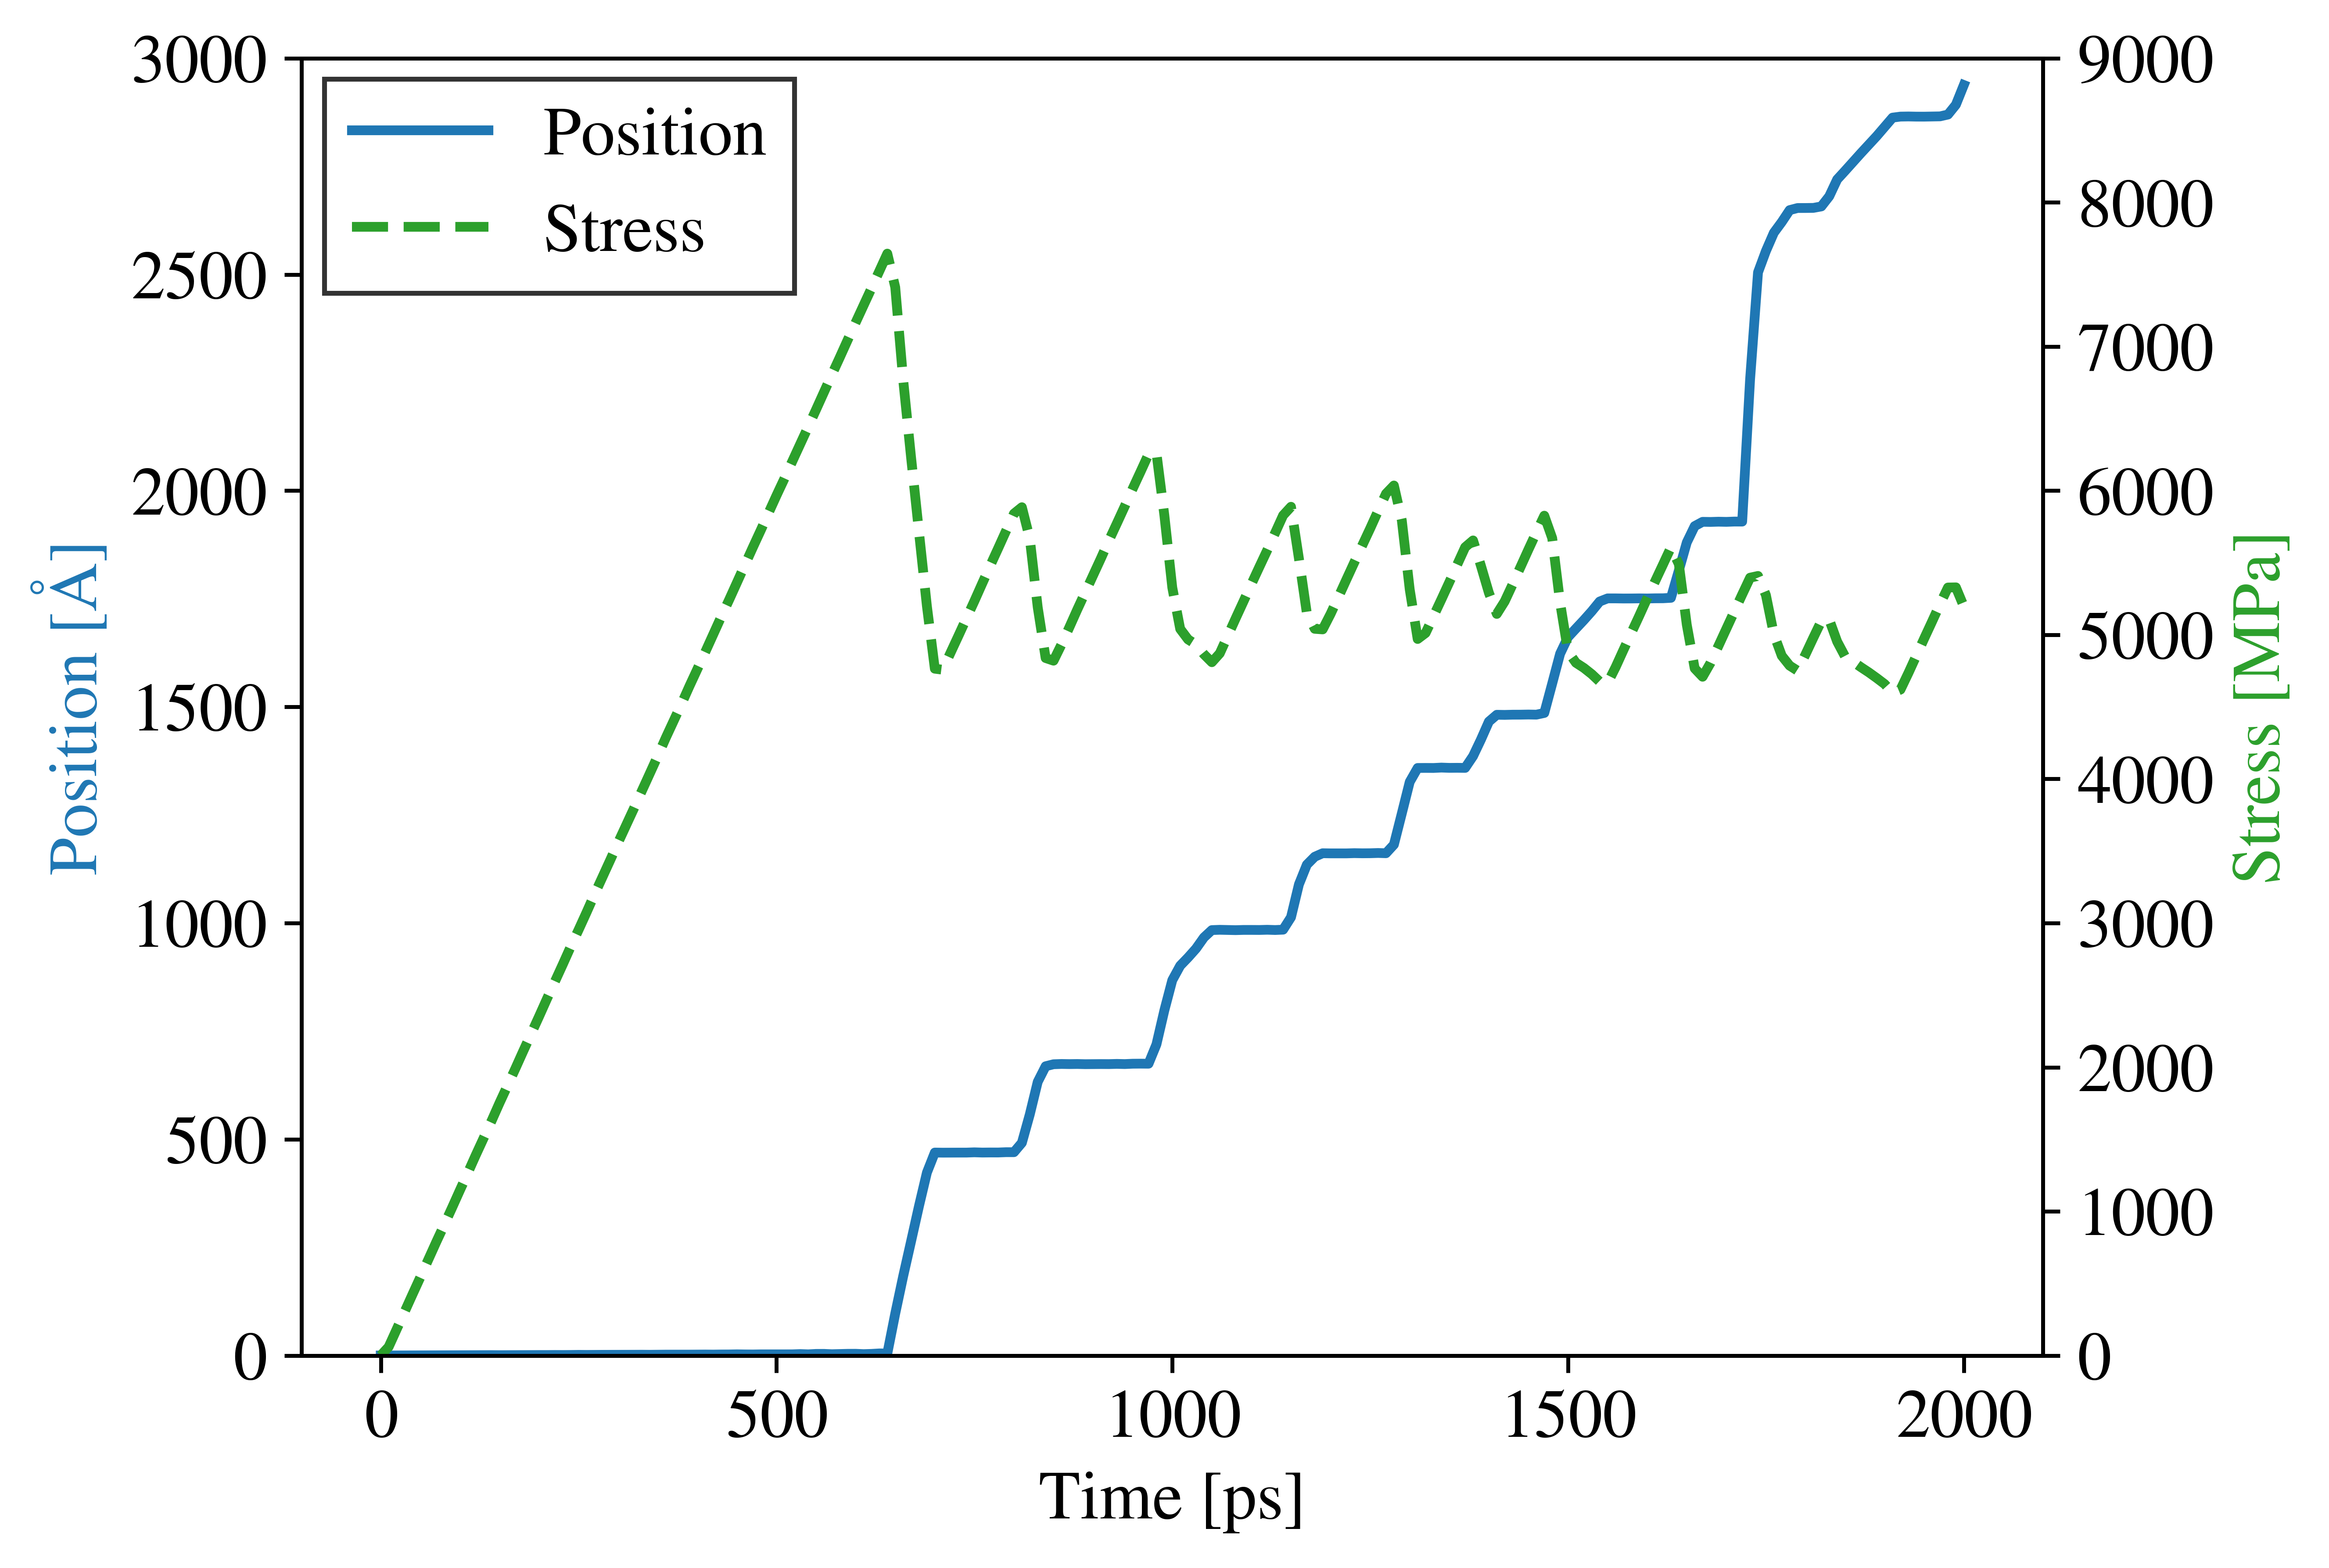
\includegraphics[width=0.48\textwidth]{Position-Stress-Edge110.png}}
\hfill
\subfloat[]{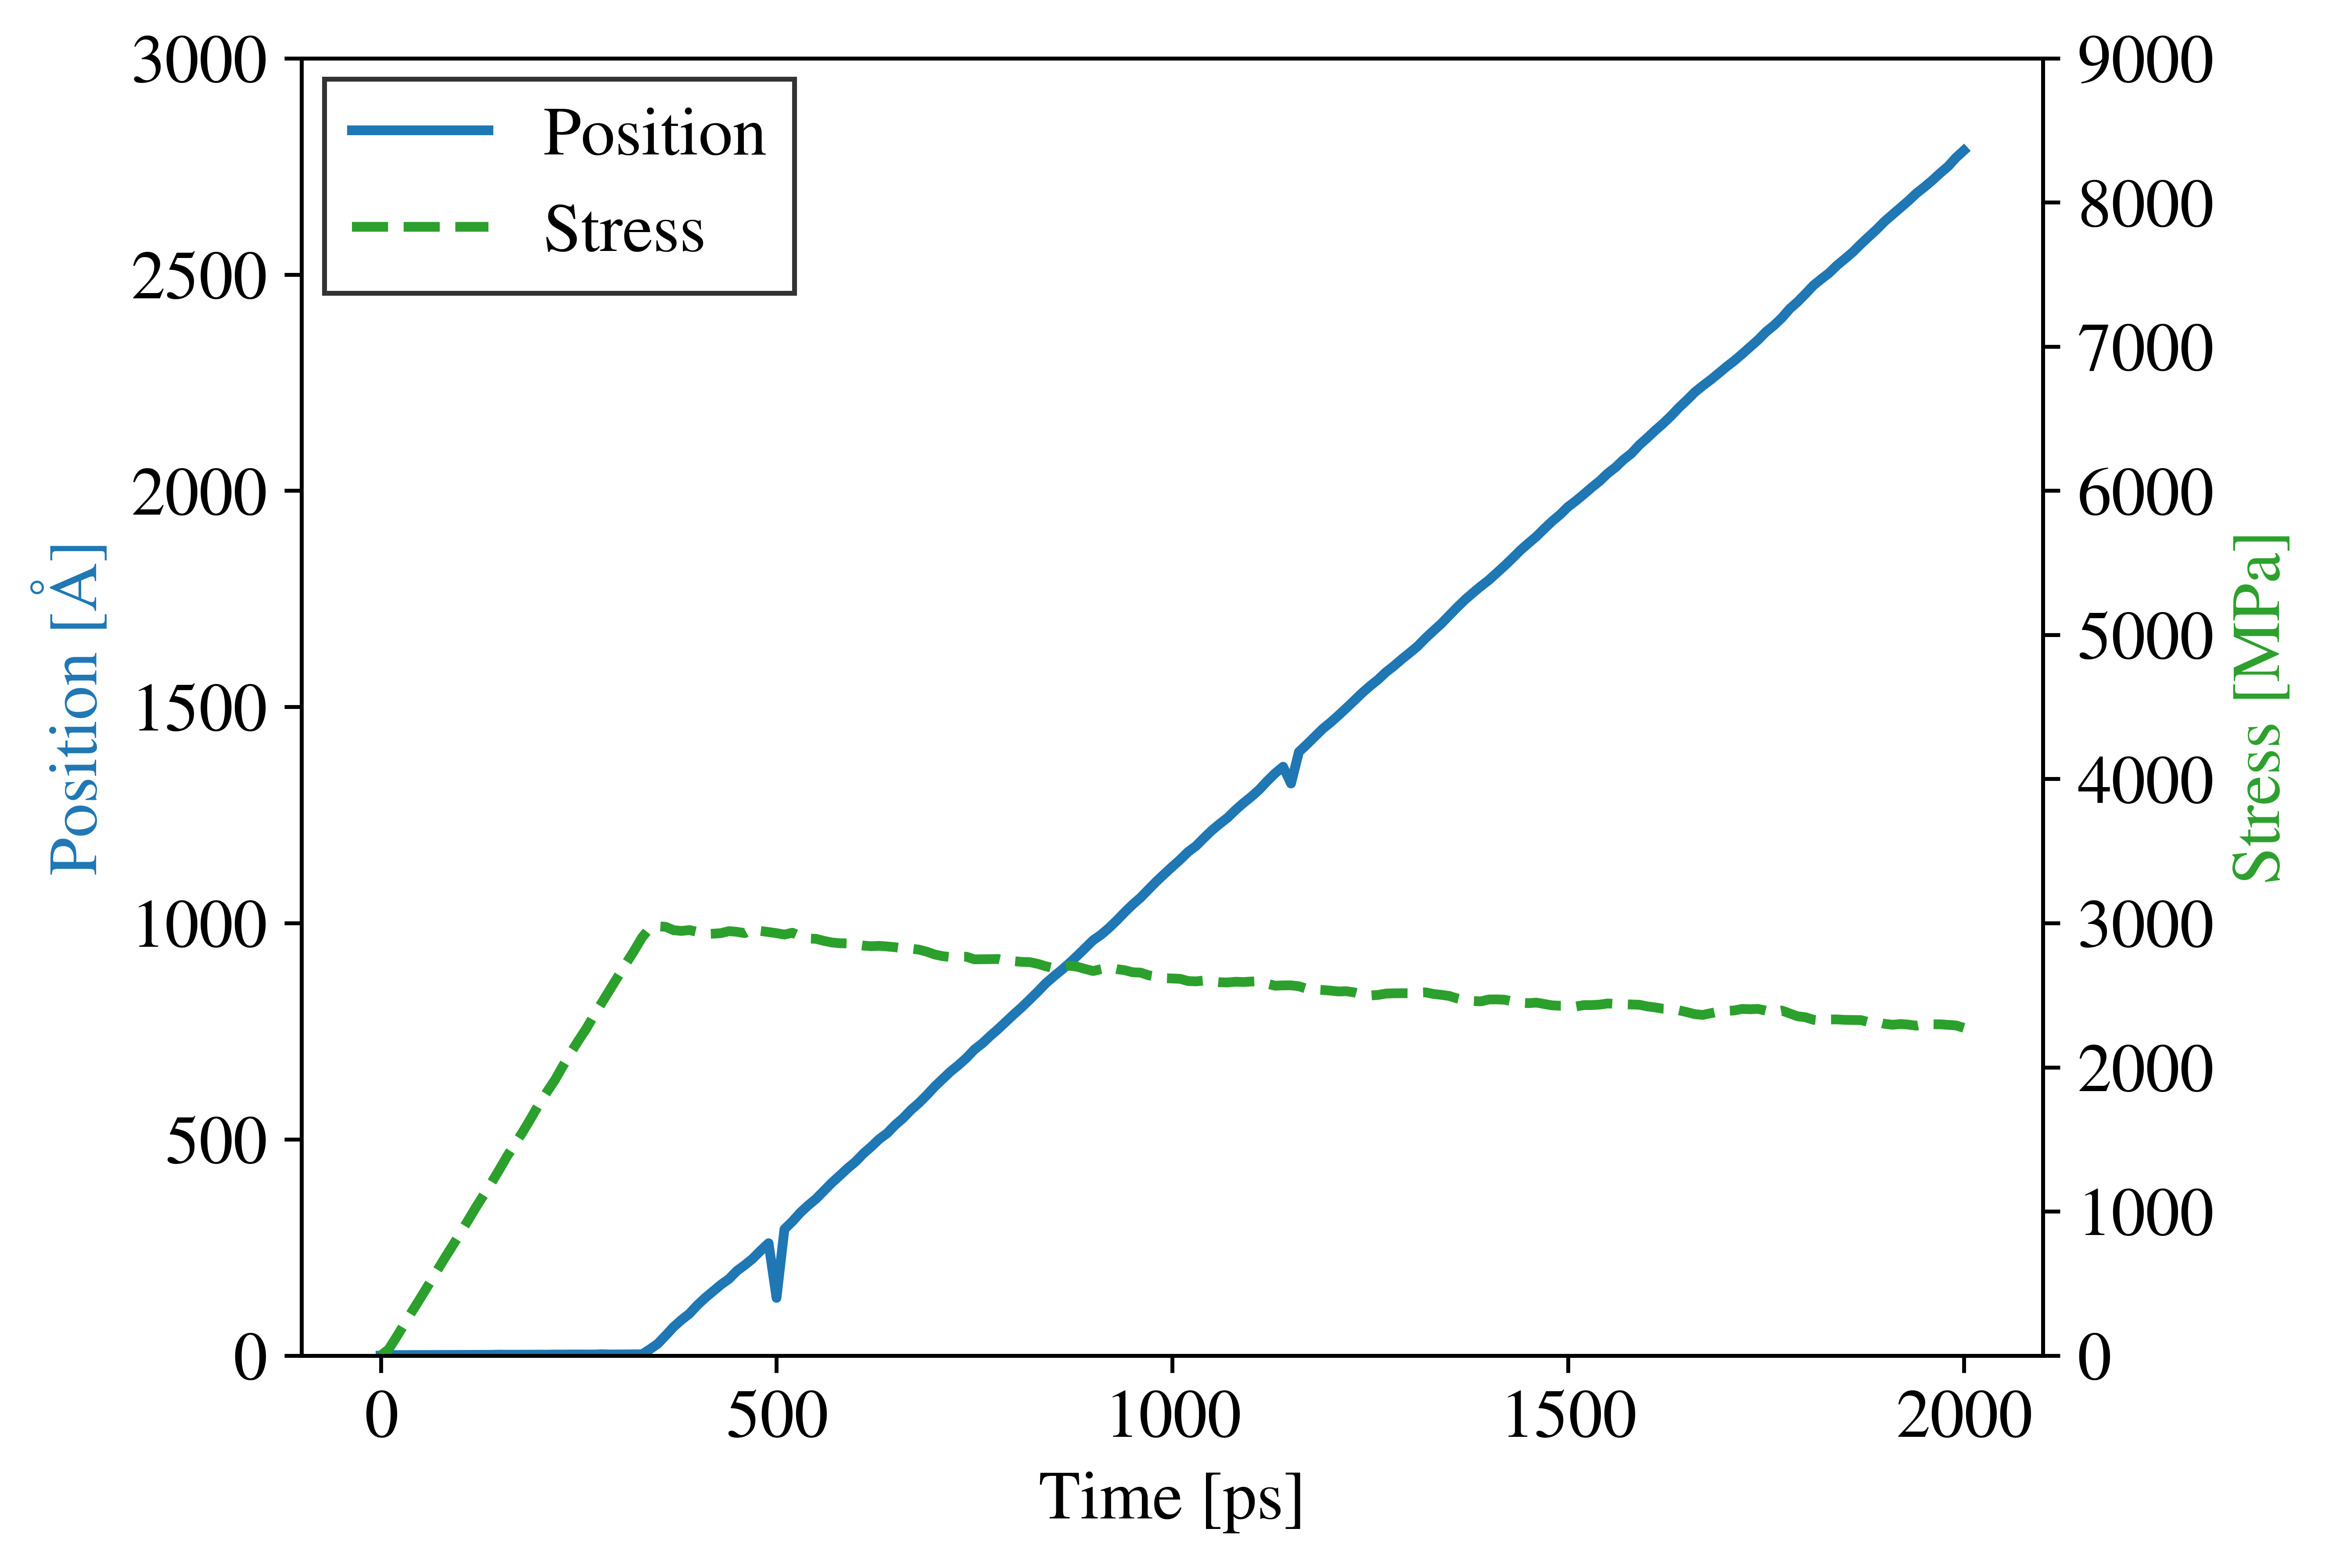
\includegraphics[width=0.48\textwidth]{Position-Stress-Edge111.png}}
\hfill
\centering\subfloat[]{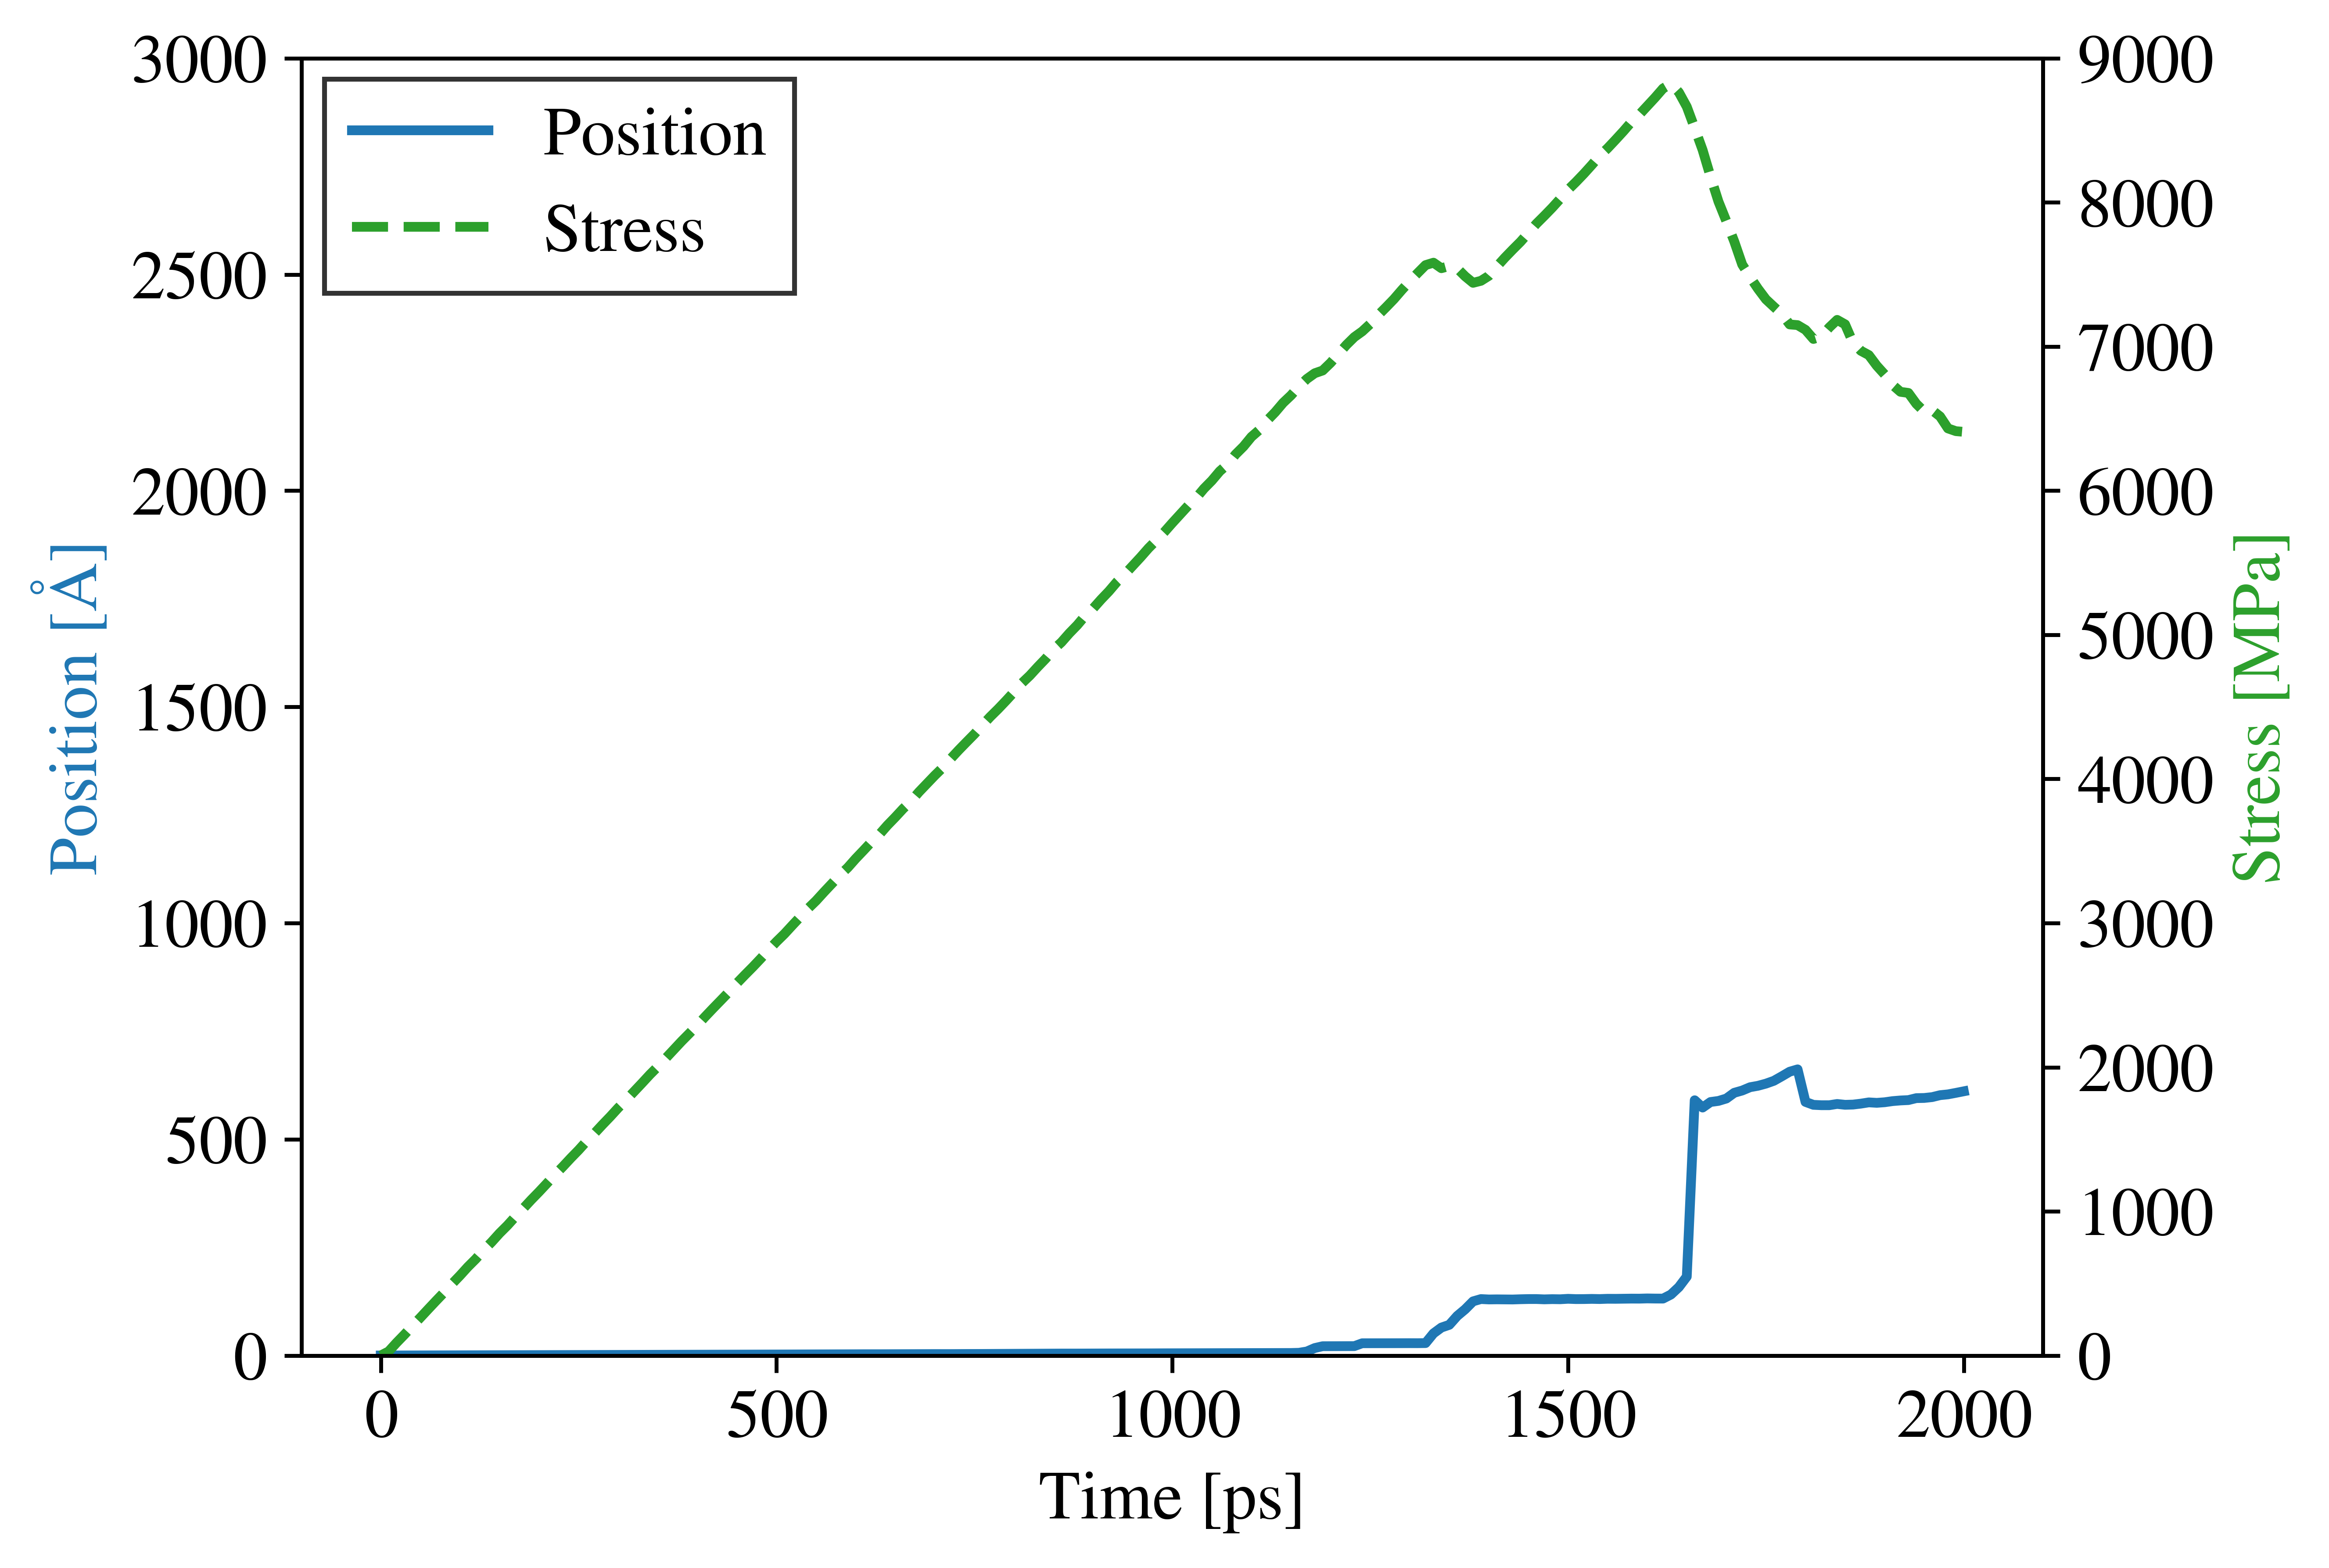
\includegraphics[width=0.48\textwidth]{Position-Stress-Edge112.png}}
}

\caption{(Color online) Movement of the $\frac{1}{2} \langle 110 \rangle$ edge dislocation along (\textbf{a}) $\{ 110 \}$, (\textbf{b}) $\{ 111 \}$, and \mbox{(\textbf{c}) $\{112\}$} slip planes under applied strain rate of $10^{-4}$ s$^{-1}$. To~calculate the Peierls stress, the~developed shear stress on each dislocation is also averaged and is shown in the~figures.}
\label{Fig:Disloc}
\end{figure}

Based on the OVITO visualization, it was observed that the edge dislocation moves via a kink-pair mechanism~\cite{Hull2011}. Assisted by thermal vibrations, the~dislocation hops from one energy minimum to the next along the slip plane by forming unstable kink pairs, which then annihilate one another. This continuous kink-pair nucleation and annihilation process reduces the threshold stress required to move the dislocation much below the Peierls stress. Although~the kink-pair nucleation mechanism at very low stresses is often observed for screw dislocations and rarely for edge dislocations due to stress fluctuations~\cite{Gilbert2011, Starikov2020}, it has been observed in atomistic simulations by Yu~et~al. \cite{Yu2009b} for edge dislocations in $\alpha$-Fe.


Due to the probabilistic nature of dislocation hopping, at~relatively low stresses ($\tau \leq 1150$ MPa) the motion is dominated by fluctuations and no steady-state velocity can be observed. When the stress is increased, fewer fluctuations are observed and a nearly steady-state velocity emerges. To~be consistent, however, we calculate the velocity at all stresses as the total distance traveled divided by the total simulation time, \mbox{i.e.,~1 ns.} The~variation in dislocation velocity with the applied shear stress at 300 K is shown in \cref{Fig:DislocPosTime}a on a linear scale and \cref{Fig:DislocPosTime}b on a semi-log scale, which is introduced to clarify the velocity trend in regime I. The~parameters resulting from fitting the velocity--stress curve to \mbox{\cref{Eq:MobI,Eq:MobII}} are summarized in \cref{Tab:DislocParams}. For~the stress range of \mbox{25--1150 MPa} (i.e., regime I), the~velocity--stress curve is fitted to \cref{Eq:MobI}, with $H_0 = 0.11$ eV, $p=0.37$, and~$q=0.62$. The~transition velocity is identified as \mbox{$v_t$ = 10.1 m/s,} which is the velocity corresponding to the transition stress $\tau_t$ = 1150 MPa. These values produce a coefficient of determination $R^2 = 99.9\%$. A~value of $H_0 = 0.11$ eV for UN is reasonable considering that the experimental values of the same parameter for LiF, NaCl, and~potassium chloride (KCl) are 0.09, 0.11, and~0.16 eV, respectively~\cite{Haasen1985}. Kink-pair formation energies are sensitive to supercell dimensions, especially the dimension along the dislocation line~\cite{Ventelon2009}. Thus, the~calculated value of $H_0$ should be treated as a first estimate, and~more research is required to test its convergence. A~value of $p = 0.37$ falls within the expected range (i.e., $0 \leq p \leq 1$). The~value of $q = 0.62$, however, is slightly underestimated relative to the expected range (i.e., $1 \leq q \leq 2$).

\begin{figure}[H]
{\captionsetup{position=bottom,justification=centering}
\subfloat[]{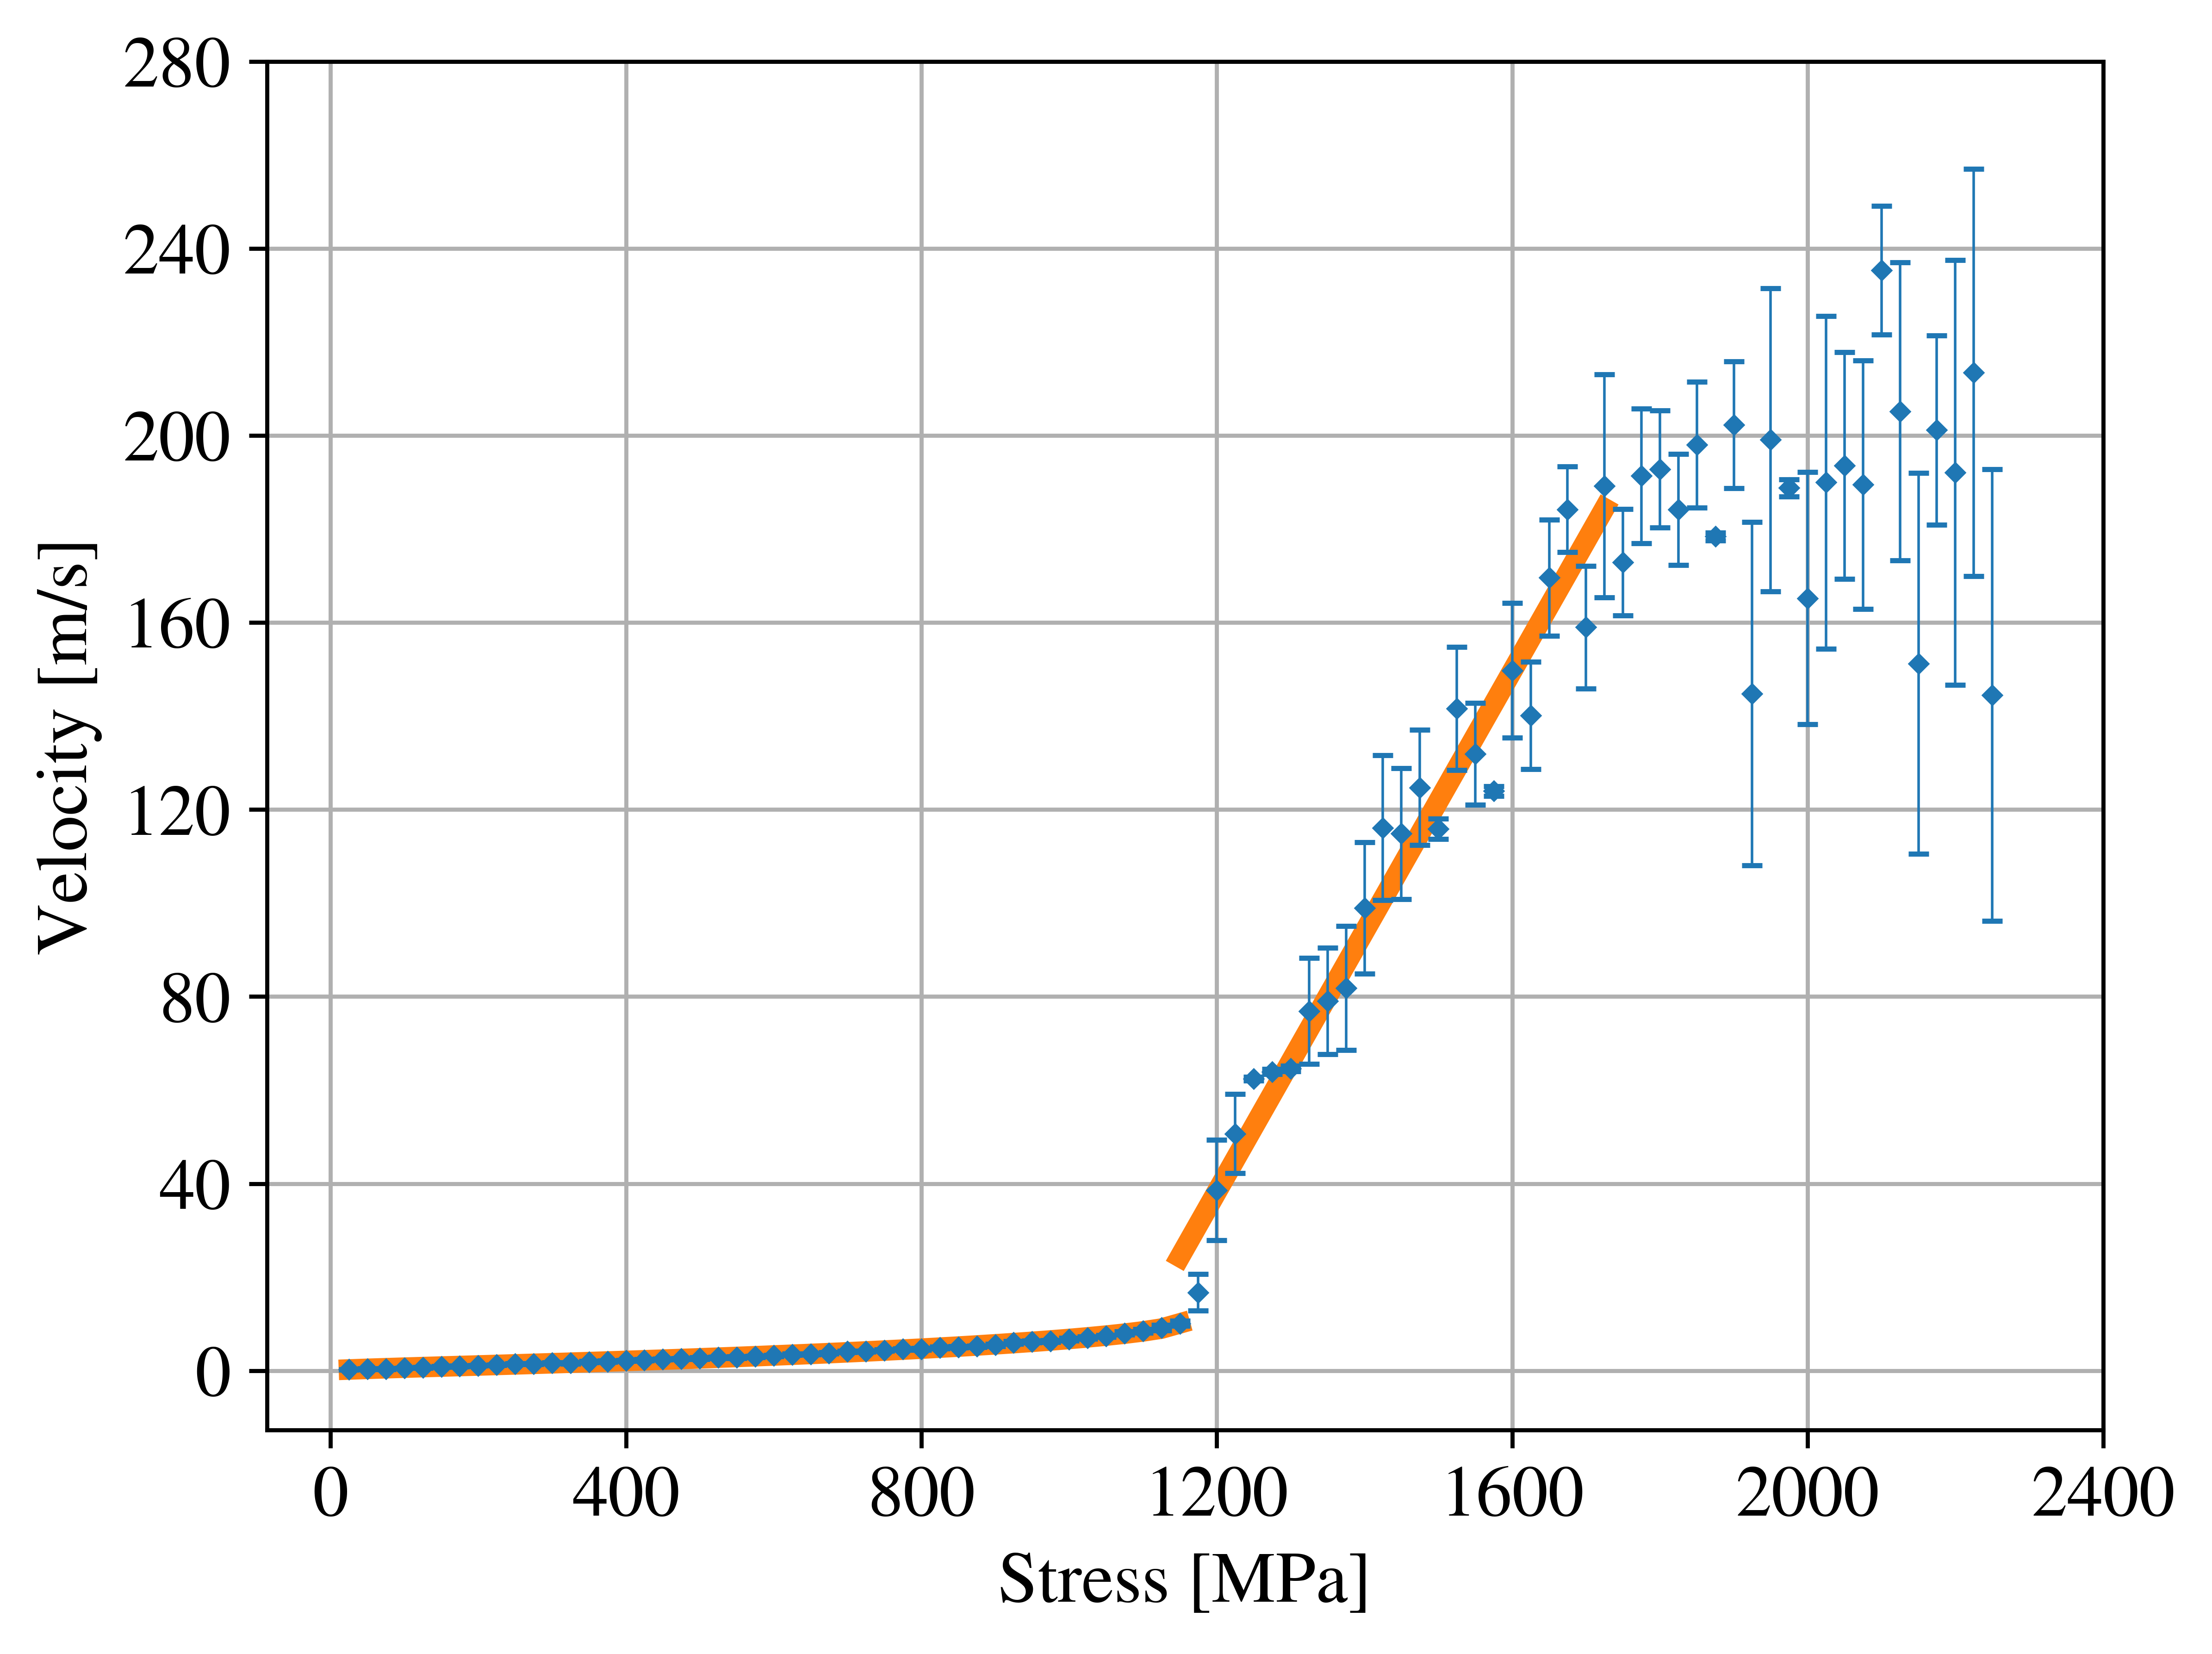
\includegraphics[width=0.48\textwidth]{DislocMob1.png}}
\hfill
\subfloat[]{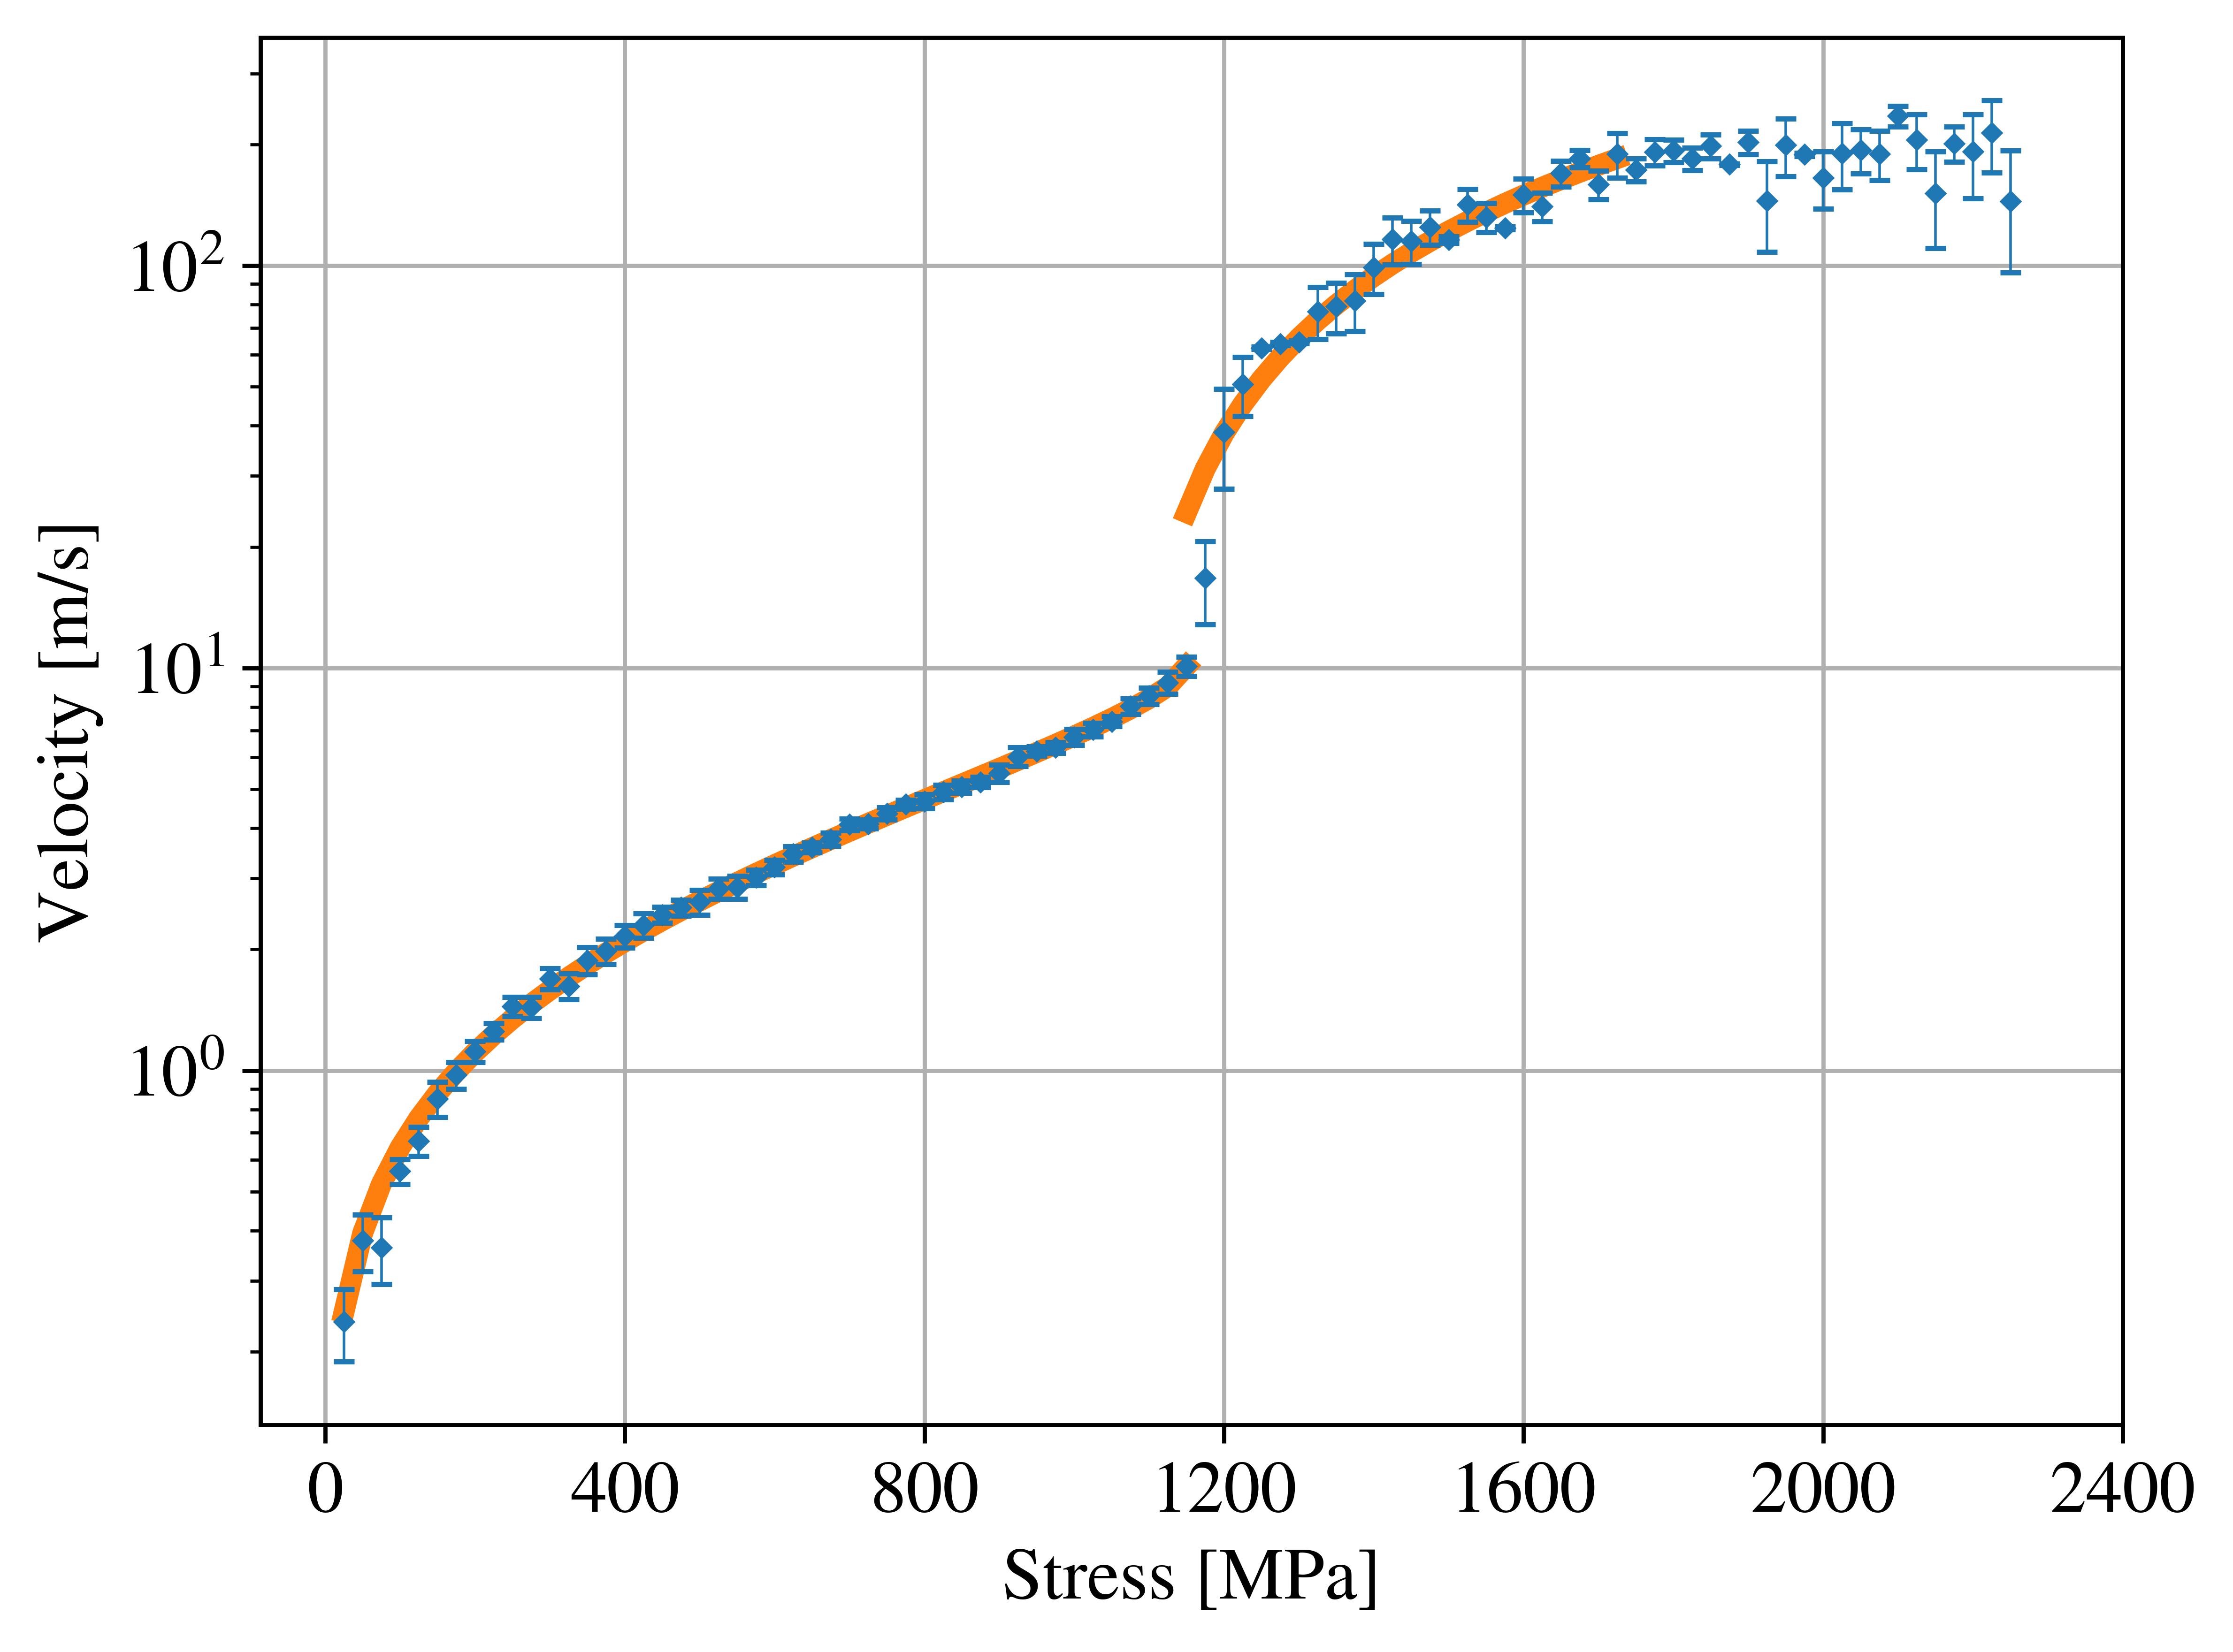
\includegraphics[width=0.48\textwidth]{DislocMob2.png}}
}
\caption{The variation in the average edge dislocation velocity in UN with shear stress (\textbf{a}) on a linear scale, and~(\textbf{b}) on a semi-log scale. The~error bars represent one standard deviation, and~the orange lines represent piecewise curve~fits.}
\label{Fig:DislocPosTime}
\end{figure}


At a stress of $\tau_t$ = 1150 MPa, a~transition to regime II occurs where the velocity varies linearly with stress. Fitting the velocity--stress curve in regime II to \cref{Eq:MobII}, we find that the phonon drag coefficient $B$ = $1.22 \times 10^{-3}$ $\mathrm{Pa} \! \cdot \! \mathrm{s}$. This value produces $R^2 = 95.8\%$. The~linear fit is valid until a stress $\tau_t'$ = 1725 MPa, where a deviation from linearity is apparent, i.e.,~a transition to regime III occurs where the uncertainty in the velocity is much higher than in regimes I and II, with a maximum standard deviation of 50 m/s. The~linear dislocation mobility is calculated to be $M = 1/B$ = 817 $\mathrm{Pa}^{-1} \! \cdot \! \mathrm{s}^{-1}$. To~give context to this value, the~mobility of edge dislocations in two iron--chromium--nickel steel systems \mbox{(i.e., \ce{Fe40Cr25Ni35}} and \ce{Fe50Cr20Ni30}) was calculated by Kaloni~et~al. \cite{Kaloni2023} to be $5.01 \times 10^4$ and $7.04 \times 10^4$ $\mathrm{Pa}^{-1} \! \cdot \! \mathrm{s}^{-1}$, respectively. This implies that UN is less ductile than steel systems, which is expected considering that UN is~ceramic.

\begin{table}[H]
\tablesize{\small}
\caption{Parameters of the mobility functions (\cref{Eq:MobI,Eq:MobII}) fitted to the motion of the $\frac{1}{2}\langle110\rangle\{111\}$ edge and $\frac{1}{2}\langle110\rangle\{110\}$ screw dislocations at 300~K.}
\newcolumntype{C}{>{\centering\arraybackslash}X}
\begin{tabularx}{\textwidth}{lcc}
\toprule
\textbf{Parameter} & \textbf{Edge Dislocation} & \textbf{Screw Dislocation} \\
\midrule
Kink-pair formation energy, $H_0$ [eV] & 0.11 & 1.0 \\
Exponent $p$ & 0.37 & 0.0037 \\
Exponent $q$ & 0.62 & 0.30 \\
Transition stress between regimes I and II, $\tau_t$ [MPa] & 1150 & 700 \\
Transition velocity between regimes I and II, $v_t$ [m/s] & 10.1 & 20.1 \\
Phonon drag coefficient, $B$ [$\mathrm{Pa} \! \cdot \! \mathrm{s}$] & $1.22 \times 10^{-3}$ & $2.20 \times 10^{-4}$ \\ 
Mobility, $M$ [$\mathrm{Pa}^{-1} \! \cdot \! \mathrm{s}^{-1}$] & 817 & 4546 \\
Additive constant, $C$ [m/s] & $-296$ & $-1134$ \\
Transition stress between regimes II and III, $\tau_t'$ [MPa] & 1725 & 1125 \\
\bottomrule
\end{tabularx}
\label{Tab:DislocParams}
\end{table}

An interesting observation is that in the linear range at intermediate stresses, the~steady-state movement of the dislocation is occasionally interrupted by abrupt jumps that occur within a small time interval of 20 ps, as shown in \cref{Fig:6}a for $\tau$ = 1525 MPa. These jumps have a velocity of 2977 $\pm$ 32 m/s independent of the applied stress. This velocity compares very well with the UN average sound velocity of 2990 m/s~\cite{Baranov2013}. While it is observed experimentally that dislocations move with the sound velocity at very high stresses~\cite{Johnston1959}, our finding suggests that at intermediate stresses, even when the edge dislocation displays a subsonic behavior, its steady-state motion can be interrupted by jumps that have a maximum velocity equal to the average sound velocity. This agrees with the picture that dislocation motion is~stochastic.

\begin{figure}[H]
{\captionsetup{position=bottom,justification=centering}
\subfloat[]{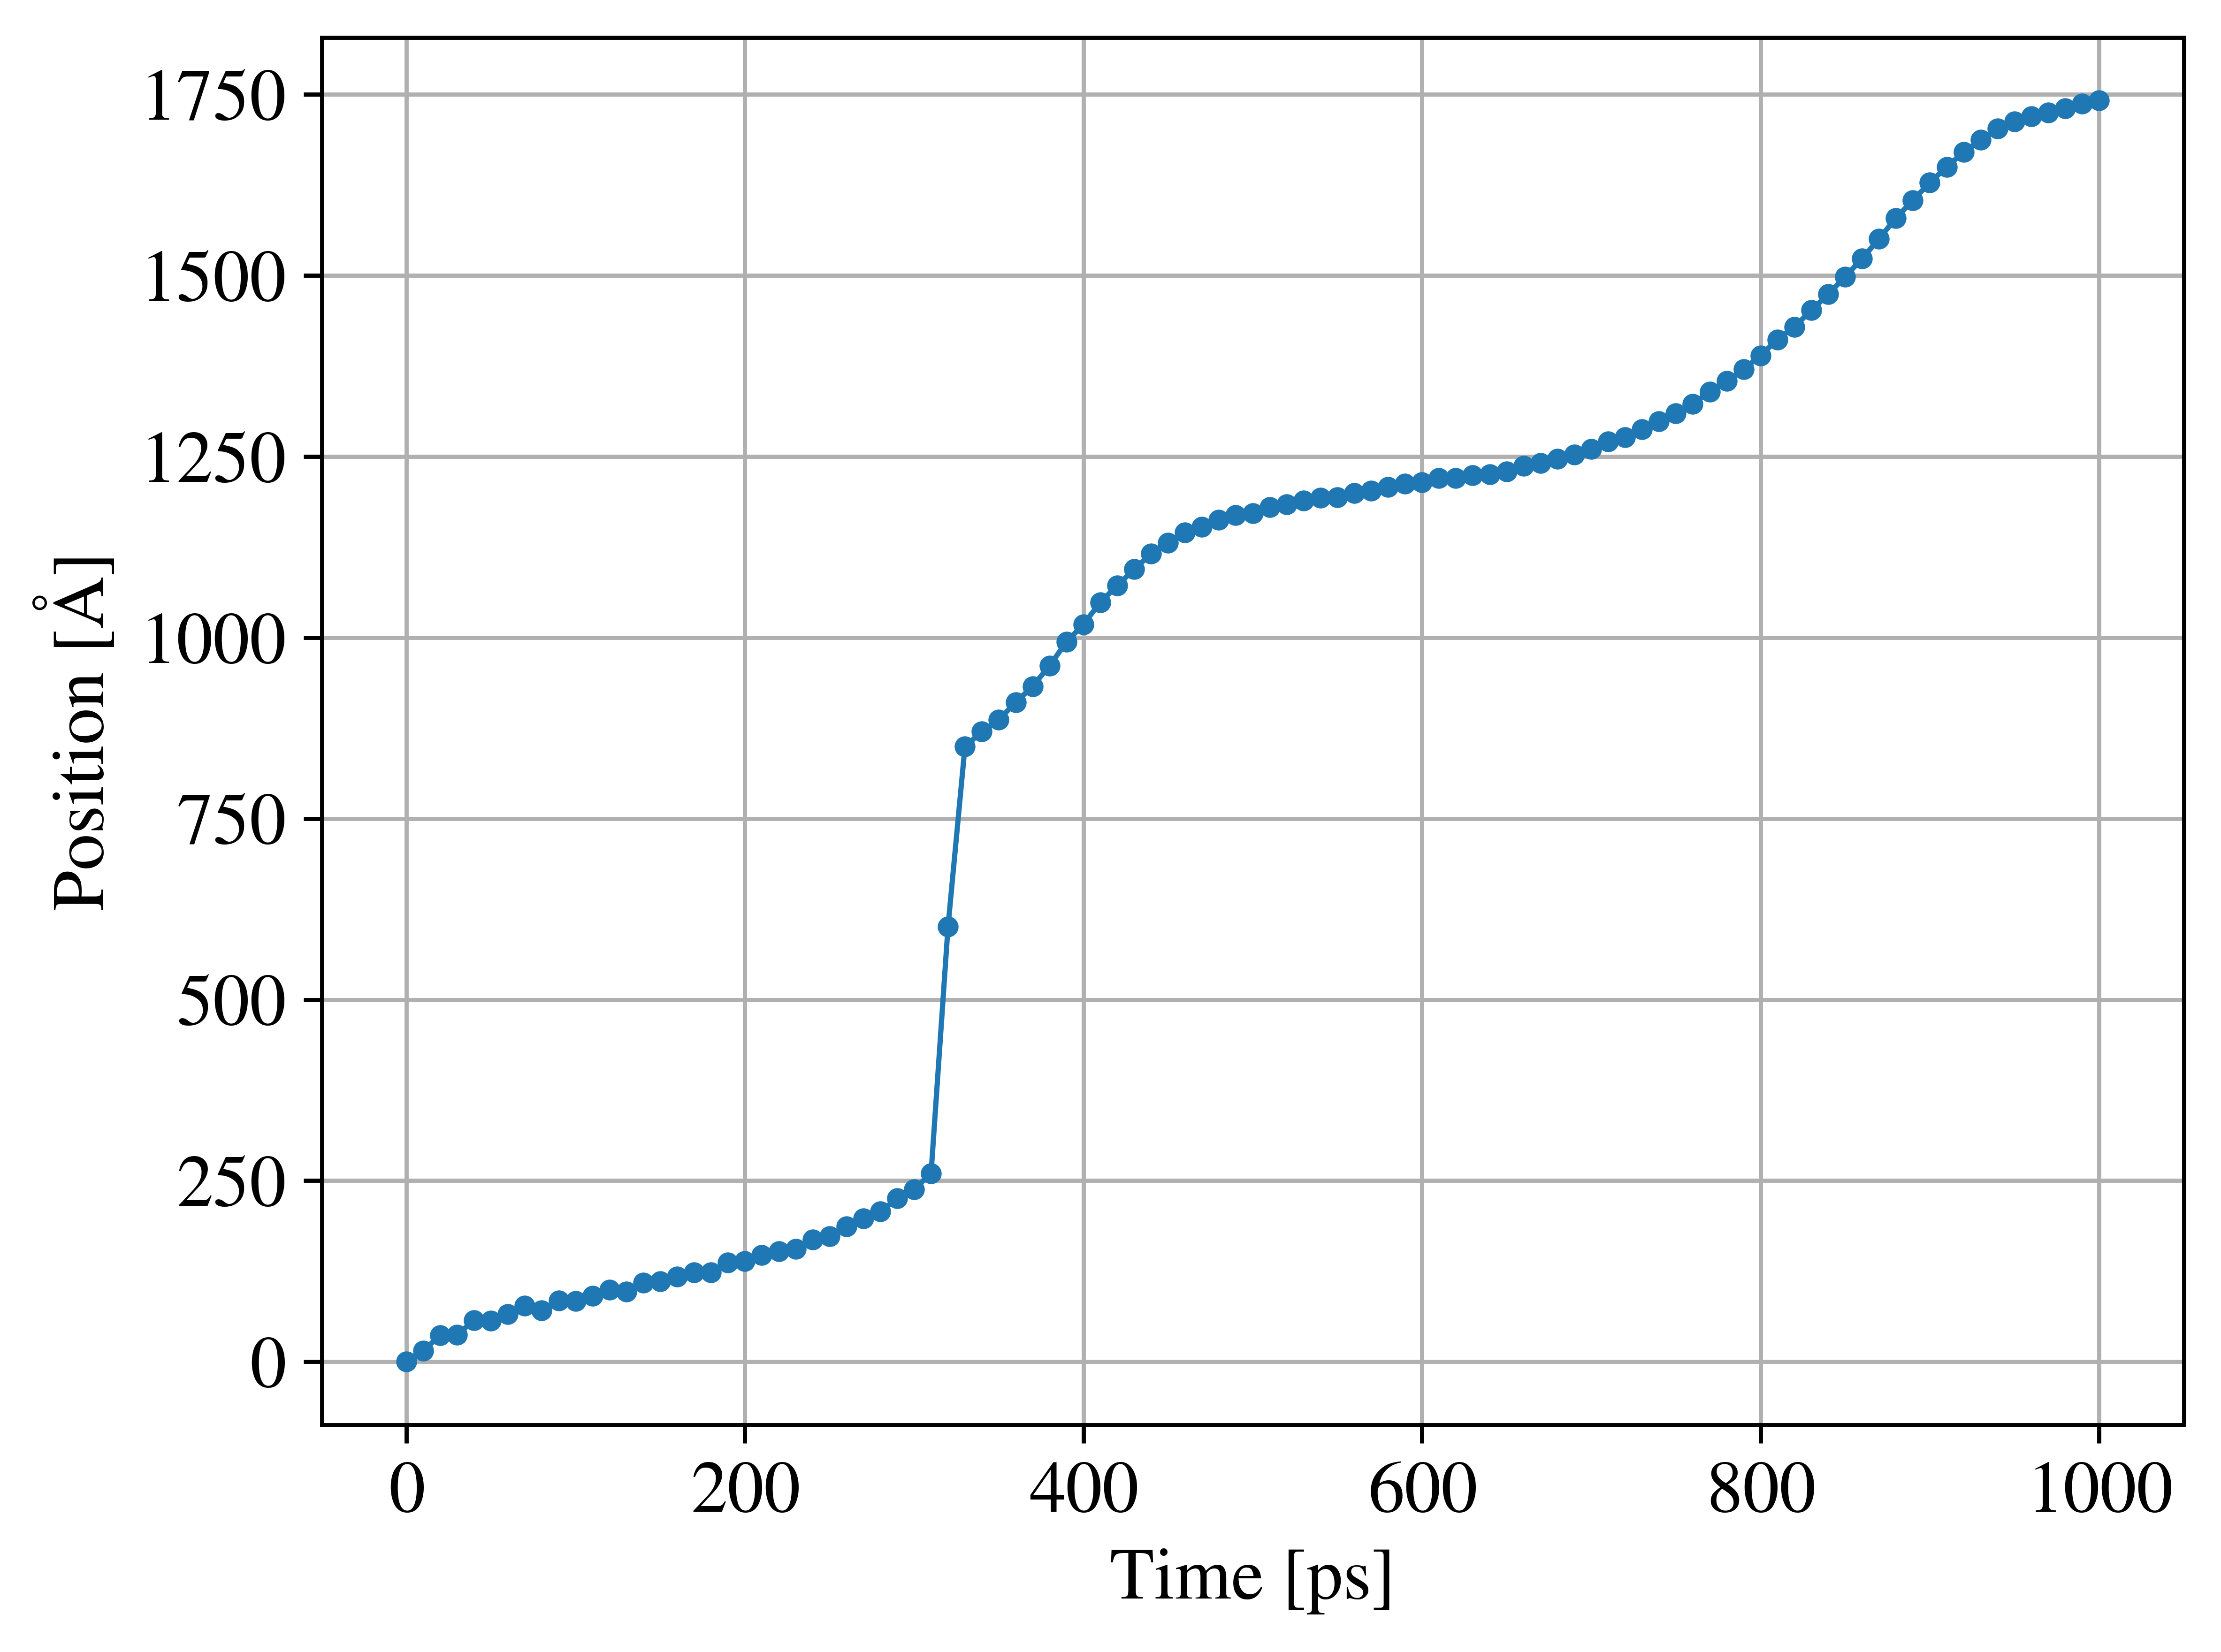
\includegraphics[width=0.48\textwidth]{Velocity-1525-MPa.png}}
\hfill
\subfloat[]{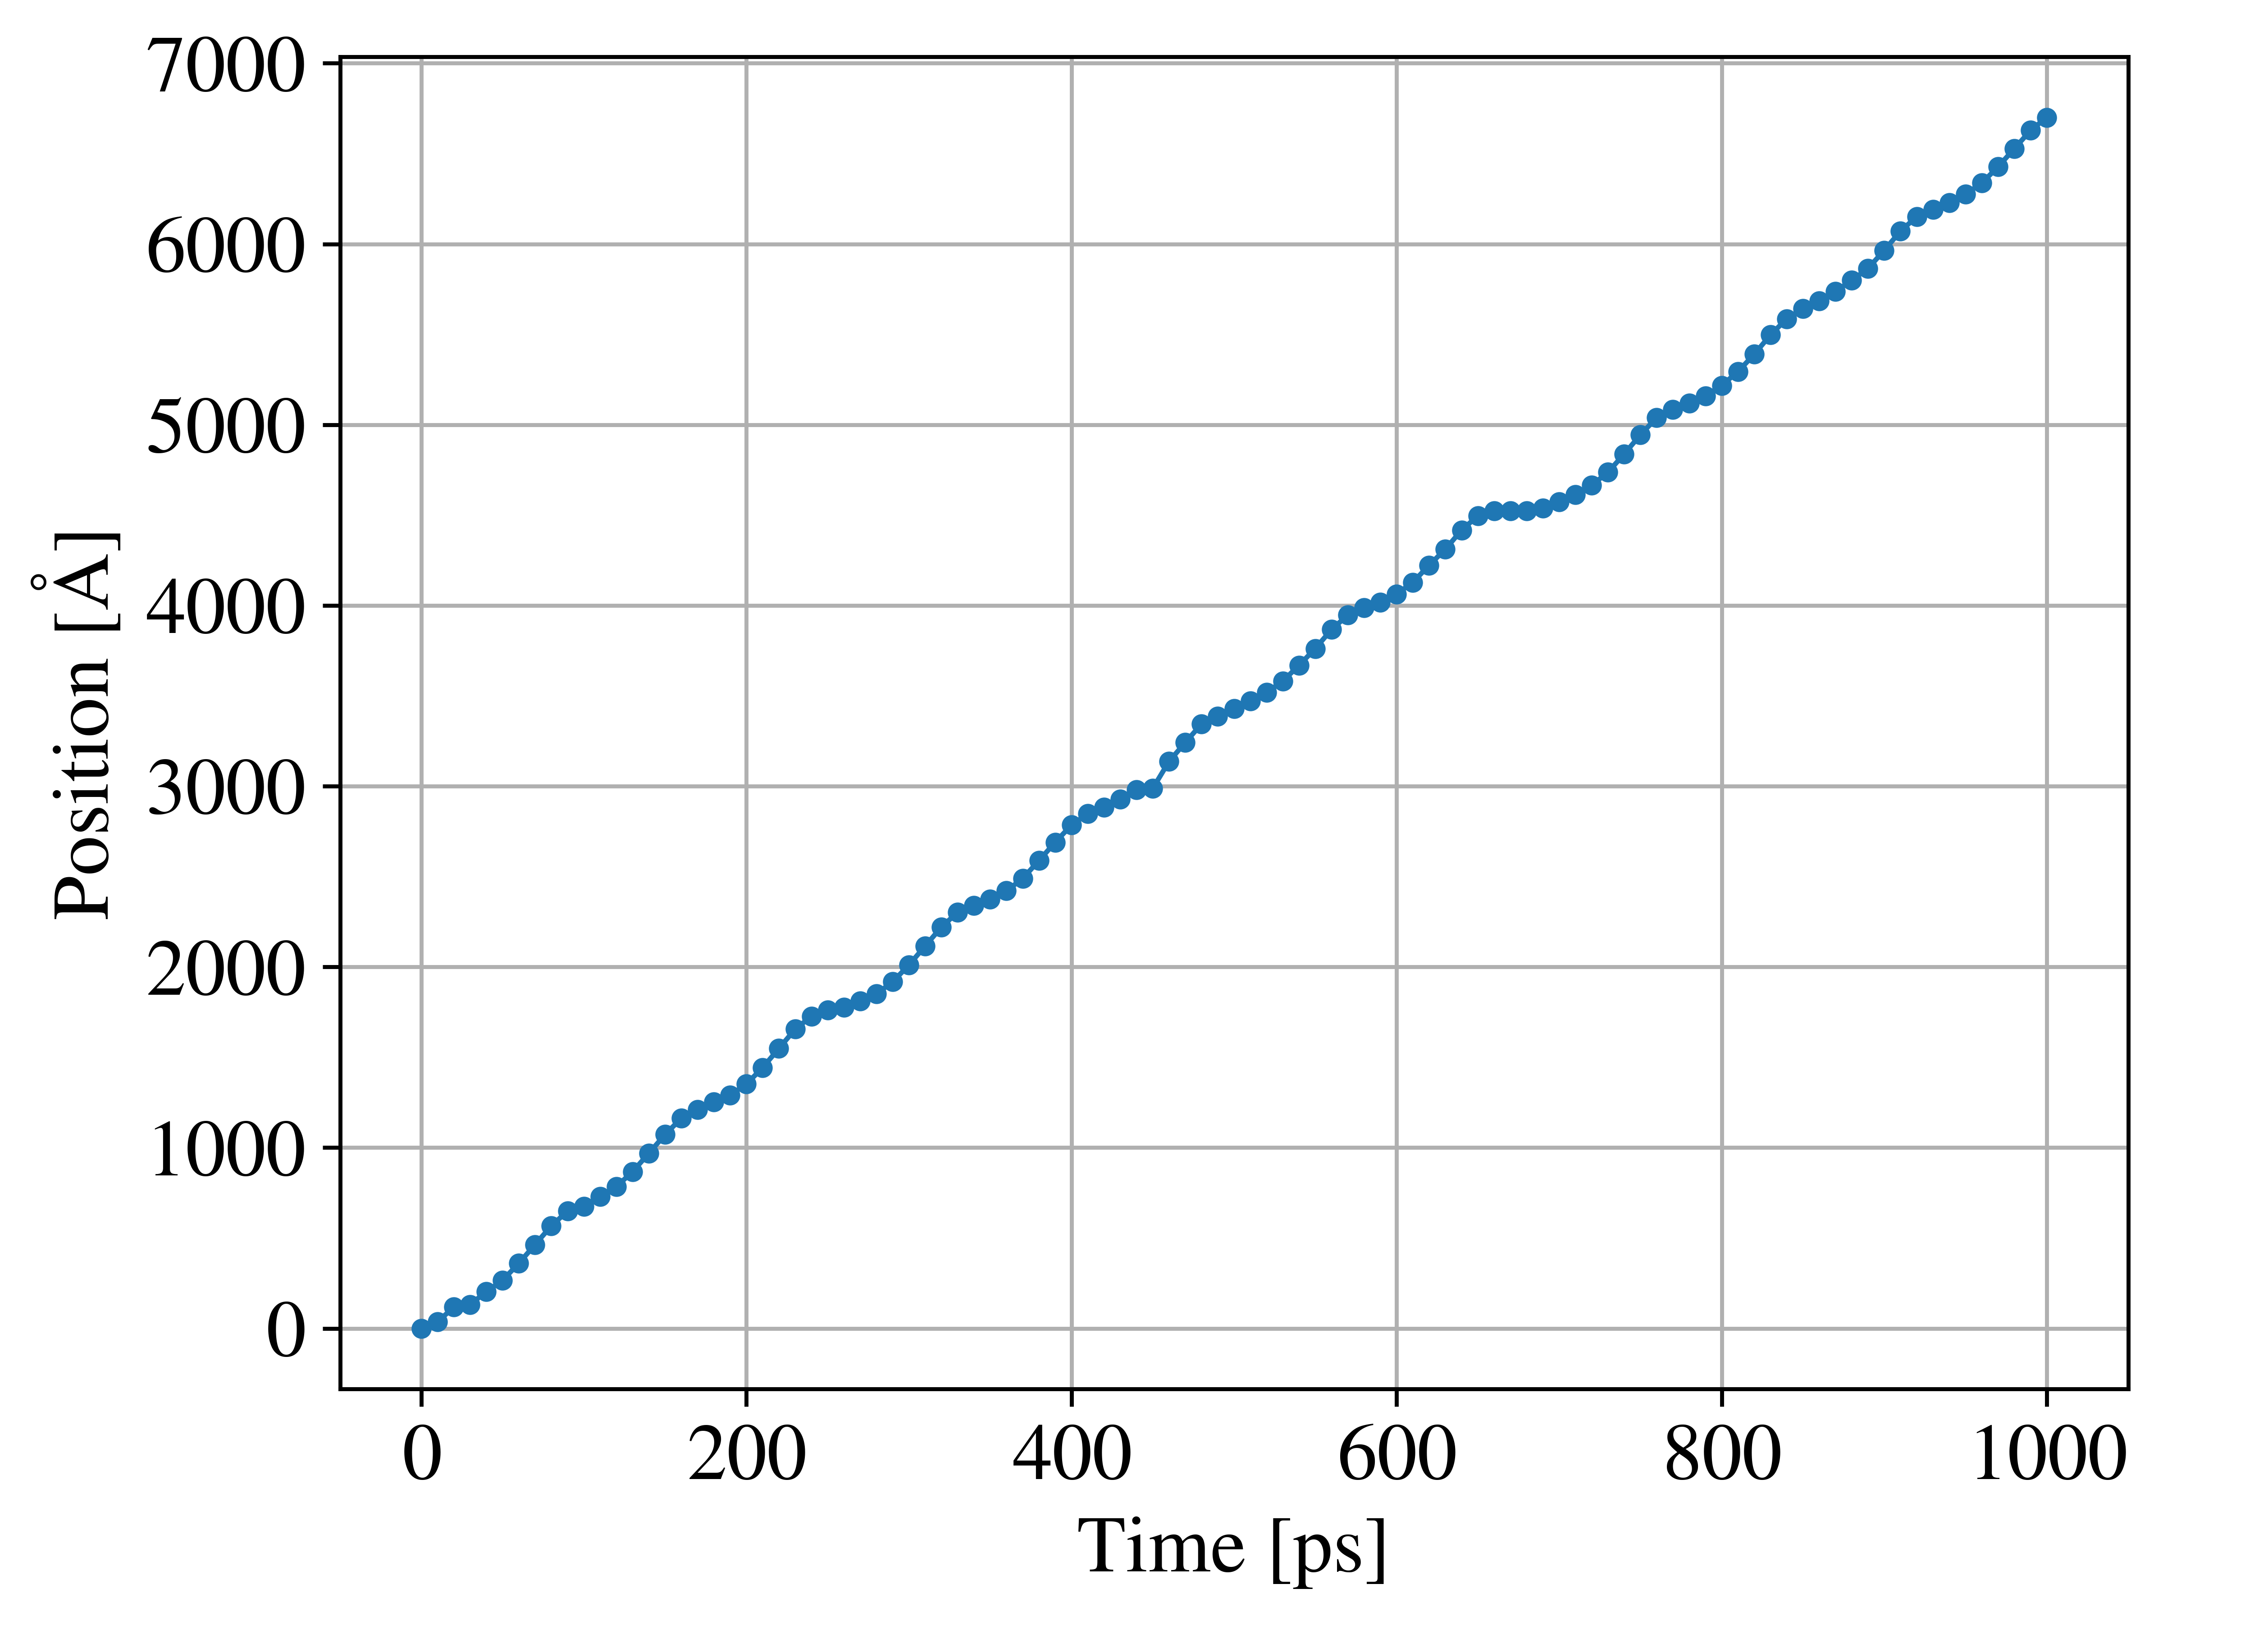
\includegraphics[width=0.48\textwidth]{Velocity-1000-MPa.png}}
}

\caption{(\textbf{a}) Position versus time profile for the movement of the $\frac{1}{2} \langle 110 \rangle \{ 111 \}$ edge dislocation under a stress of 1525 MPa. (\textbf{b}) Position versus time profile for the movement of the $\frac{1}{2} \langle 110 \rangle \{ 110 \}$ screw dislocation under a stress of 1000~MPa.}
\label{Fig:6}
\end{figure}
%\unskip

\subsubsection{Screw~Dislocations}

For the screw dislocations simulated using the Kocevski potential, we aimed to calculate the Peierls stress at 1 K for the $\{110\}$, $\{111\}$, and~$\{112\}$ planes. The~$\frac{1}{2} \langle 110 \rangle$ screw dislocation moved smoothly along the $\{110\}$ plane, as~illustrated in \cref{Fig:Screw1K}. When the dislocation was set to move along the $\{111\}$ and $\{112\}$ planes using the Kocevski potential, it was observed to cross-slip onto planes that form angles of 35.3$^\circ$ and 54.7$^\circ$ with the $\{111\}$ and $\{112\}$ planes, respectively. These angles precisely correspond to the angles between these planes and the $\{110\}$ plane. Thus, the~Kocevski potential predicts that the $\{110\}$ plane is the primary slip plane of UN, despite its inability to predict any dynamic behavior, as discussed in \cref{Sec:SS}, or to stabilize edge~dislocations.

%\begin{comment}
%
%\begin{figure}[H]
%\centering
%\begin{subfloat}{0.48\textwidth}
%    \includegraphics[width=\textwidth]{EAMScrew111.png}
%    \caption{$xz$-plane = $\{111\}$}
%\end{subfloat}
%\hfill
%\begin{subfloat}{0.48\textwidth}
%    \includegraphics[width=\textwidth]{EAMScrew112.png}
%    \caption{$xz$-plane = $\{112\}$}
%\end{subfloat}
%\caption{Snapshots of the position of the $\frac{1}{2} \langle 110 \rangle$ screw dislocation when set up to move along a (a) $\{ 111 \}$ plane and (b) $\{ 112 \}$ plane under a $\Dot{\epsilon}_{yz}$ = $10^{-4}$ s$^{-1}$ at 1 K using the Kocevski potential. In~both cases, the~$\{111\}$ and $\{ 112 \}$ planes coincide with the $xz$-plane of the supercell. The~cross in the middle of the supercell is the initial position of the screw dislocation, and~the blue dot is its position after a simulation time of 0.5 ns. The~screw dislocation cross-slips to planes that form angles of 35.3$^\circ$ and 54.7$^\circ$ with the $\{111\}$ and $\{112\}$ planes, both of which correspond to a $\{110\}$ plane.}
%\label{EAMScrew}
%\end{figure}
%
%\end{comment}



\begin{figure}[H]
    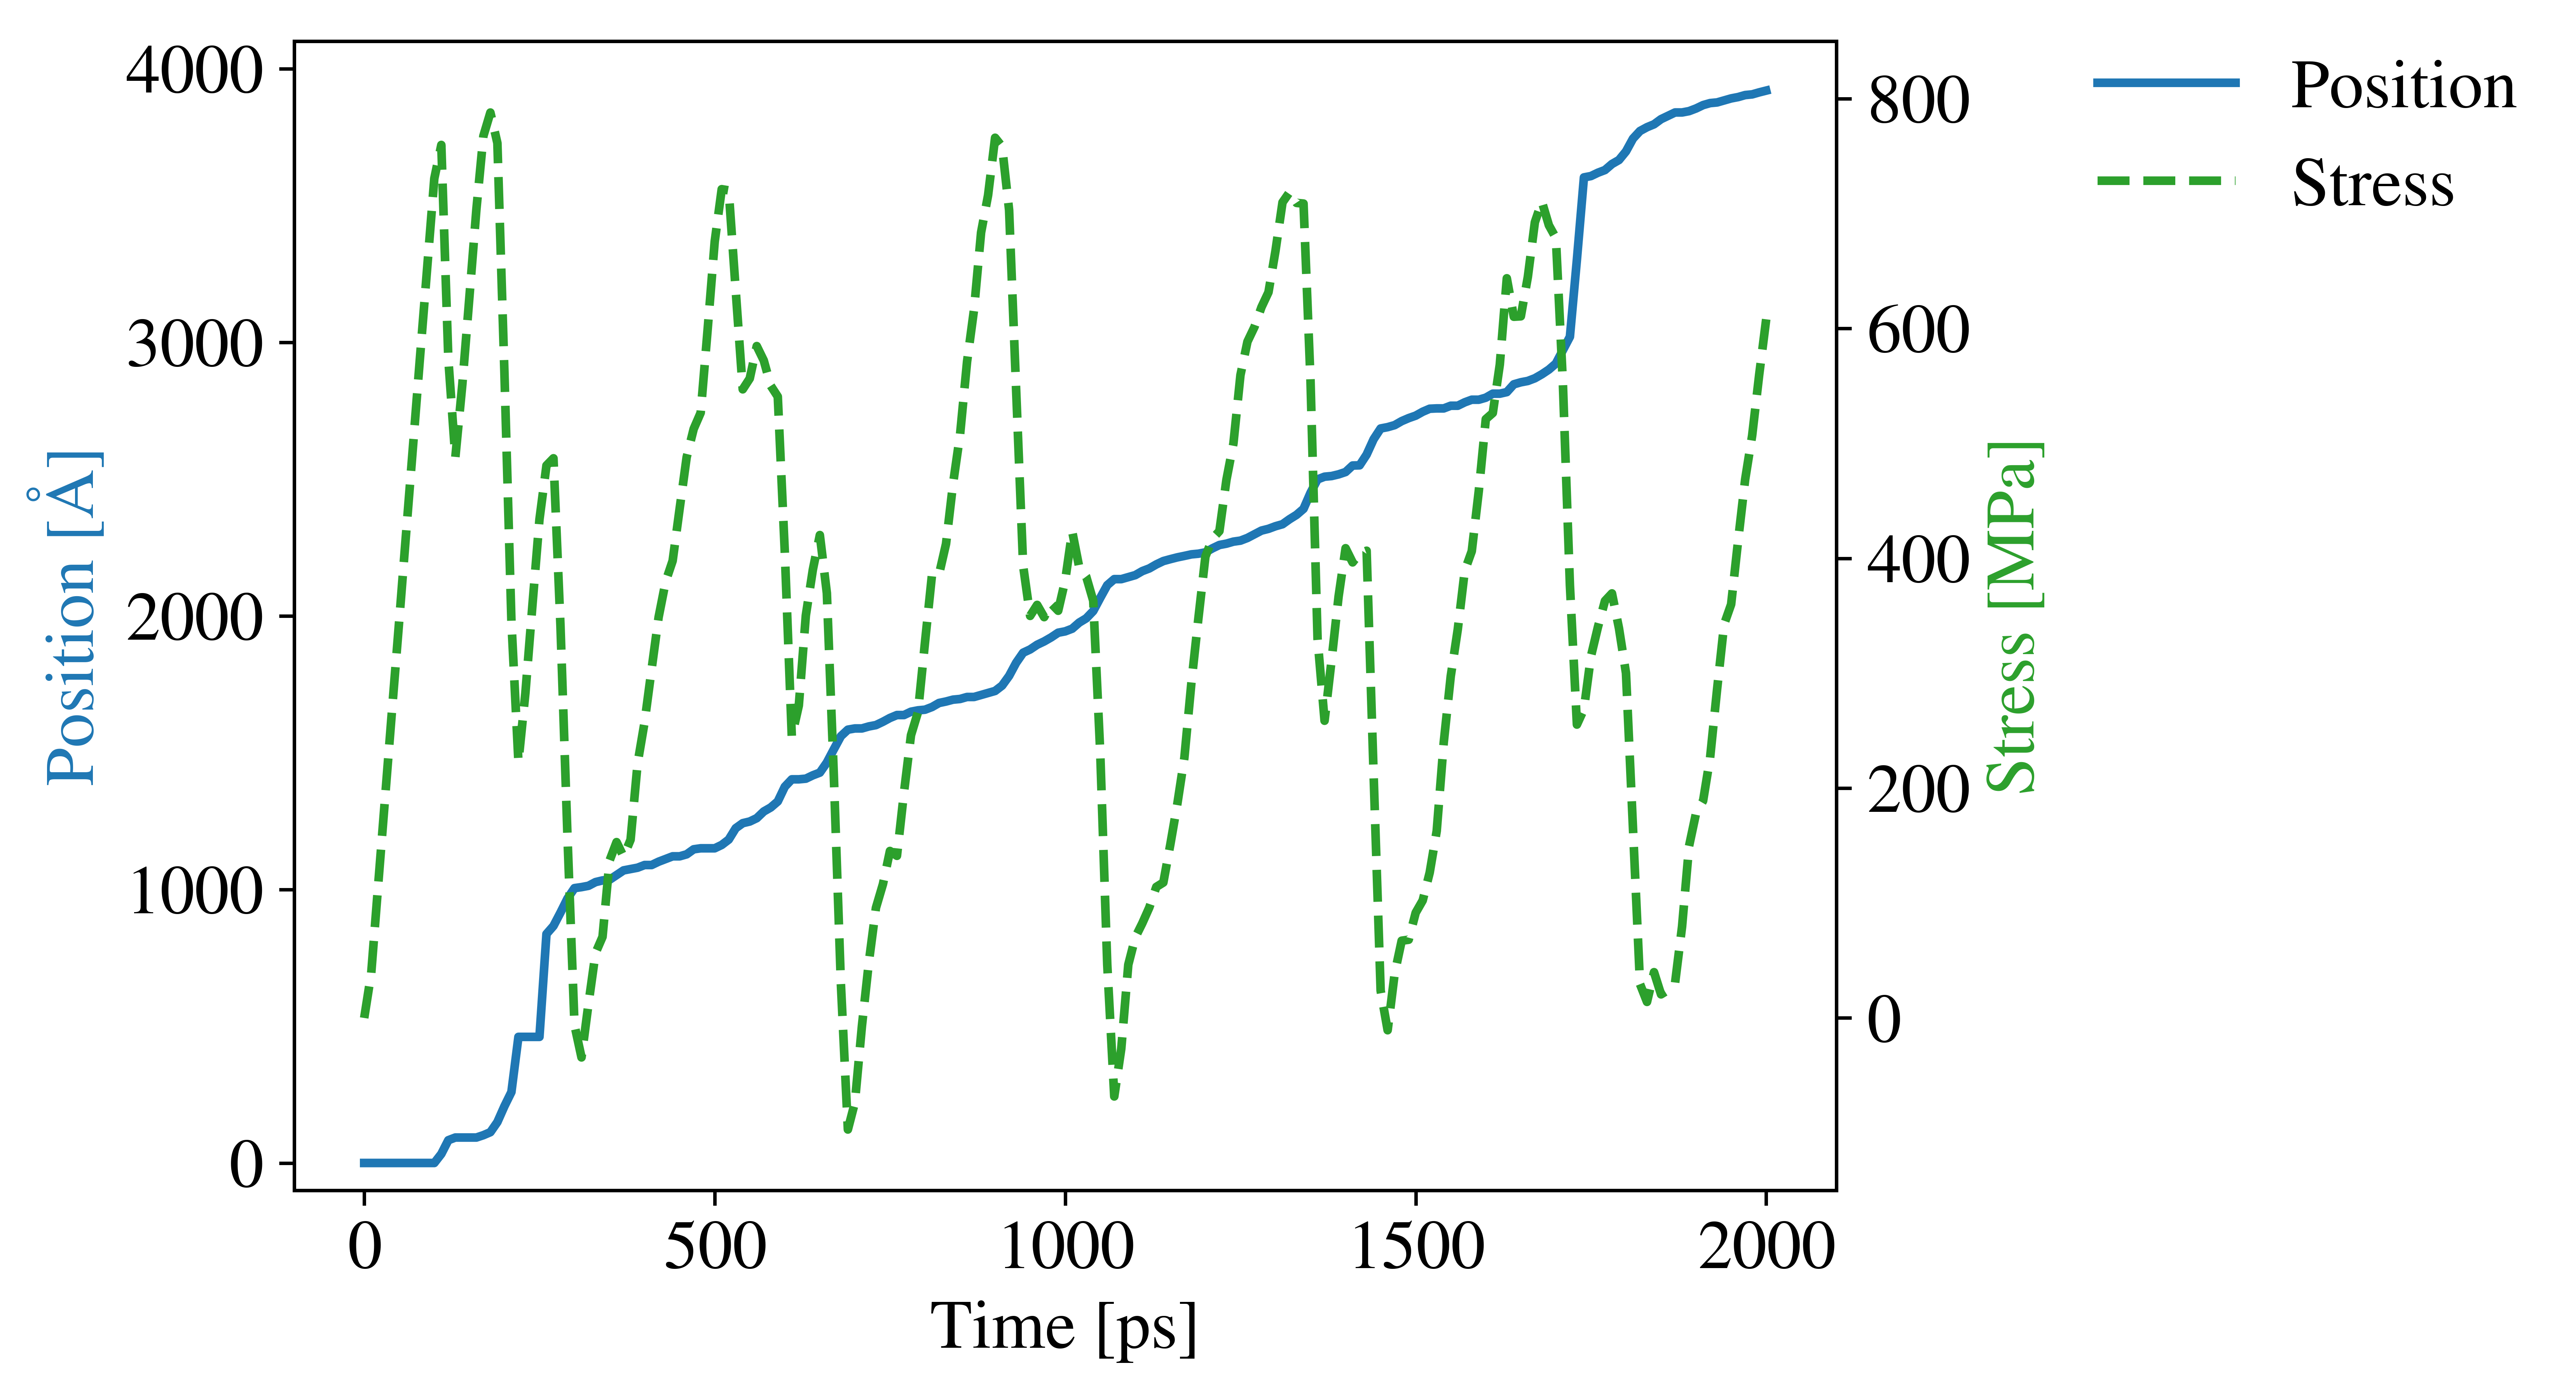
\includegraphics[width=0.8\textwidth]{Position-Stress-ScrewEAM110.png}
    \caption{Movement of the $\frac{1}{2} \langle 110 \rangle \{110\}$ screw dislocation at 1 K under an applied strain rate of \mbox{$10^{-4}$ s$^{-1}$} as predicted by the Kocevski potential. The~average of the developed $\sigma_{yz}$ stress on the dislocation is also~shown.}
    \label{Fig:Screw1K}
\end{figure}

As opposed to the GPa stresses at which the edge dislocations move at 1 K under the Tseplyaev potential, the~screw dislocation starts moving when the stress reaches 760 MPa (\cref{Fig:Screw1K}). The~maximum value of the stress is 790 MPa, which we designate as the Peierls stress for the screw dislocation. Despite the large stress fluctuations, this value is surprisingly relevant to the mobility calculation and corresponds to the transition stress from regime I to regime II. Only the movement along the $\{110\}$ planes is used to fit a mobility function for the screw~dislocation.


The motion of the screw dislocation was tracked under constant stress in the range of 25--1200 MPa at 300 K, and~an example of such a calculation is shown in \cref{Fig:6}b. The~results of the mobility calculation for the screw dislocation are shown in \cref{Fig:DislocPosTimeScrew}. At~stresses smaller than 100 MPa, the~screw dislocation oscillates around its initial position without any observable motion. At~stresses between 100 and 200 MPa, the~screw dislocation performs only a few jumps on the time scale of 1 ns, which results in average velocities in the order of $10^{-1}$ m/s. Between~200 and 700 MPa, motion by the kink-pair mechanism is observed. We fitted \cref{Eq:MobII} to the data points in the 200--700 MPa region and found that $H_0$ = 1.0 eV, $p$ = 0.00037, and~$q$ = 0.30. These values have an $R^2$ = 98.3\%. $p$~falls within the expected range of 0--1, although~its significantly small value indicates a minor stress dependence. As~for the edge dislocation, $q$ is underestimated compared to its expected range of 1--2. $H_0$ for the screw dislocation is larger than that of the edge dislocation (0.11~eV). However, the~transition velocity to regime II, i.e.,~$v_t$ = 22.1 m/s, is larger than that of the edge dislocation (10.1 m/s) while the transition stress is smaller (700 MPa for the screw dislocation versus 1150 MPa for the edge dislocation). For~the stress range 700--1125 MPa, the~velocity varies linearly with the stress (regime II) and values of $M$ = 4546 $\mathrm{Pa}^{-1} \! \cdot \! \mathrm{s}^{-1}$ and $C = - 1134$ m/s fit the data points in this regime to \cref{Eq:MobII} with $R^2$ = 94.8\%. For~stresses larger than 1125 MPa, debris production was observed in the wake of the dislocation, which reduced the velocity. The~fitting parameters of the screw dislocation mobility function are shown in \cref{Tab:DislocParams}. The~linear mobility of the screw dislocation is larger than that of the edge dislocation by more than a factor of 5. Despite the usual caveats expected in comparing the qualitative results of two different interatomic potentials, we can expect, based on the results, that the screw dislocations most likely dominate the deformation process in UN. This picture agrees with the experimental observation that dislocations in UN are nearly pure screws~\cite{Sole1968}.

\begin{figure}[H]
{\captionsetup{position=bottom,justification=centering}
\subfloat[]{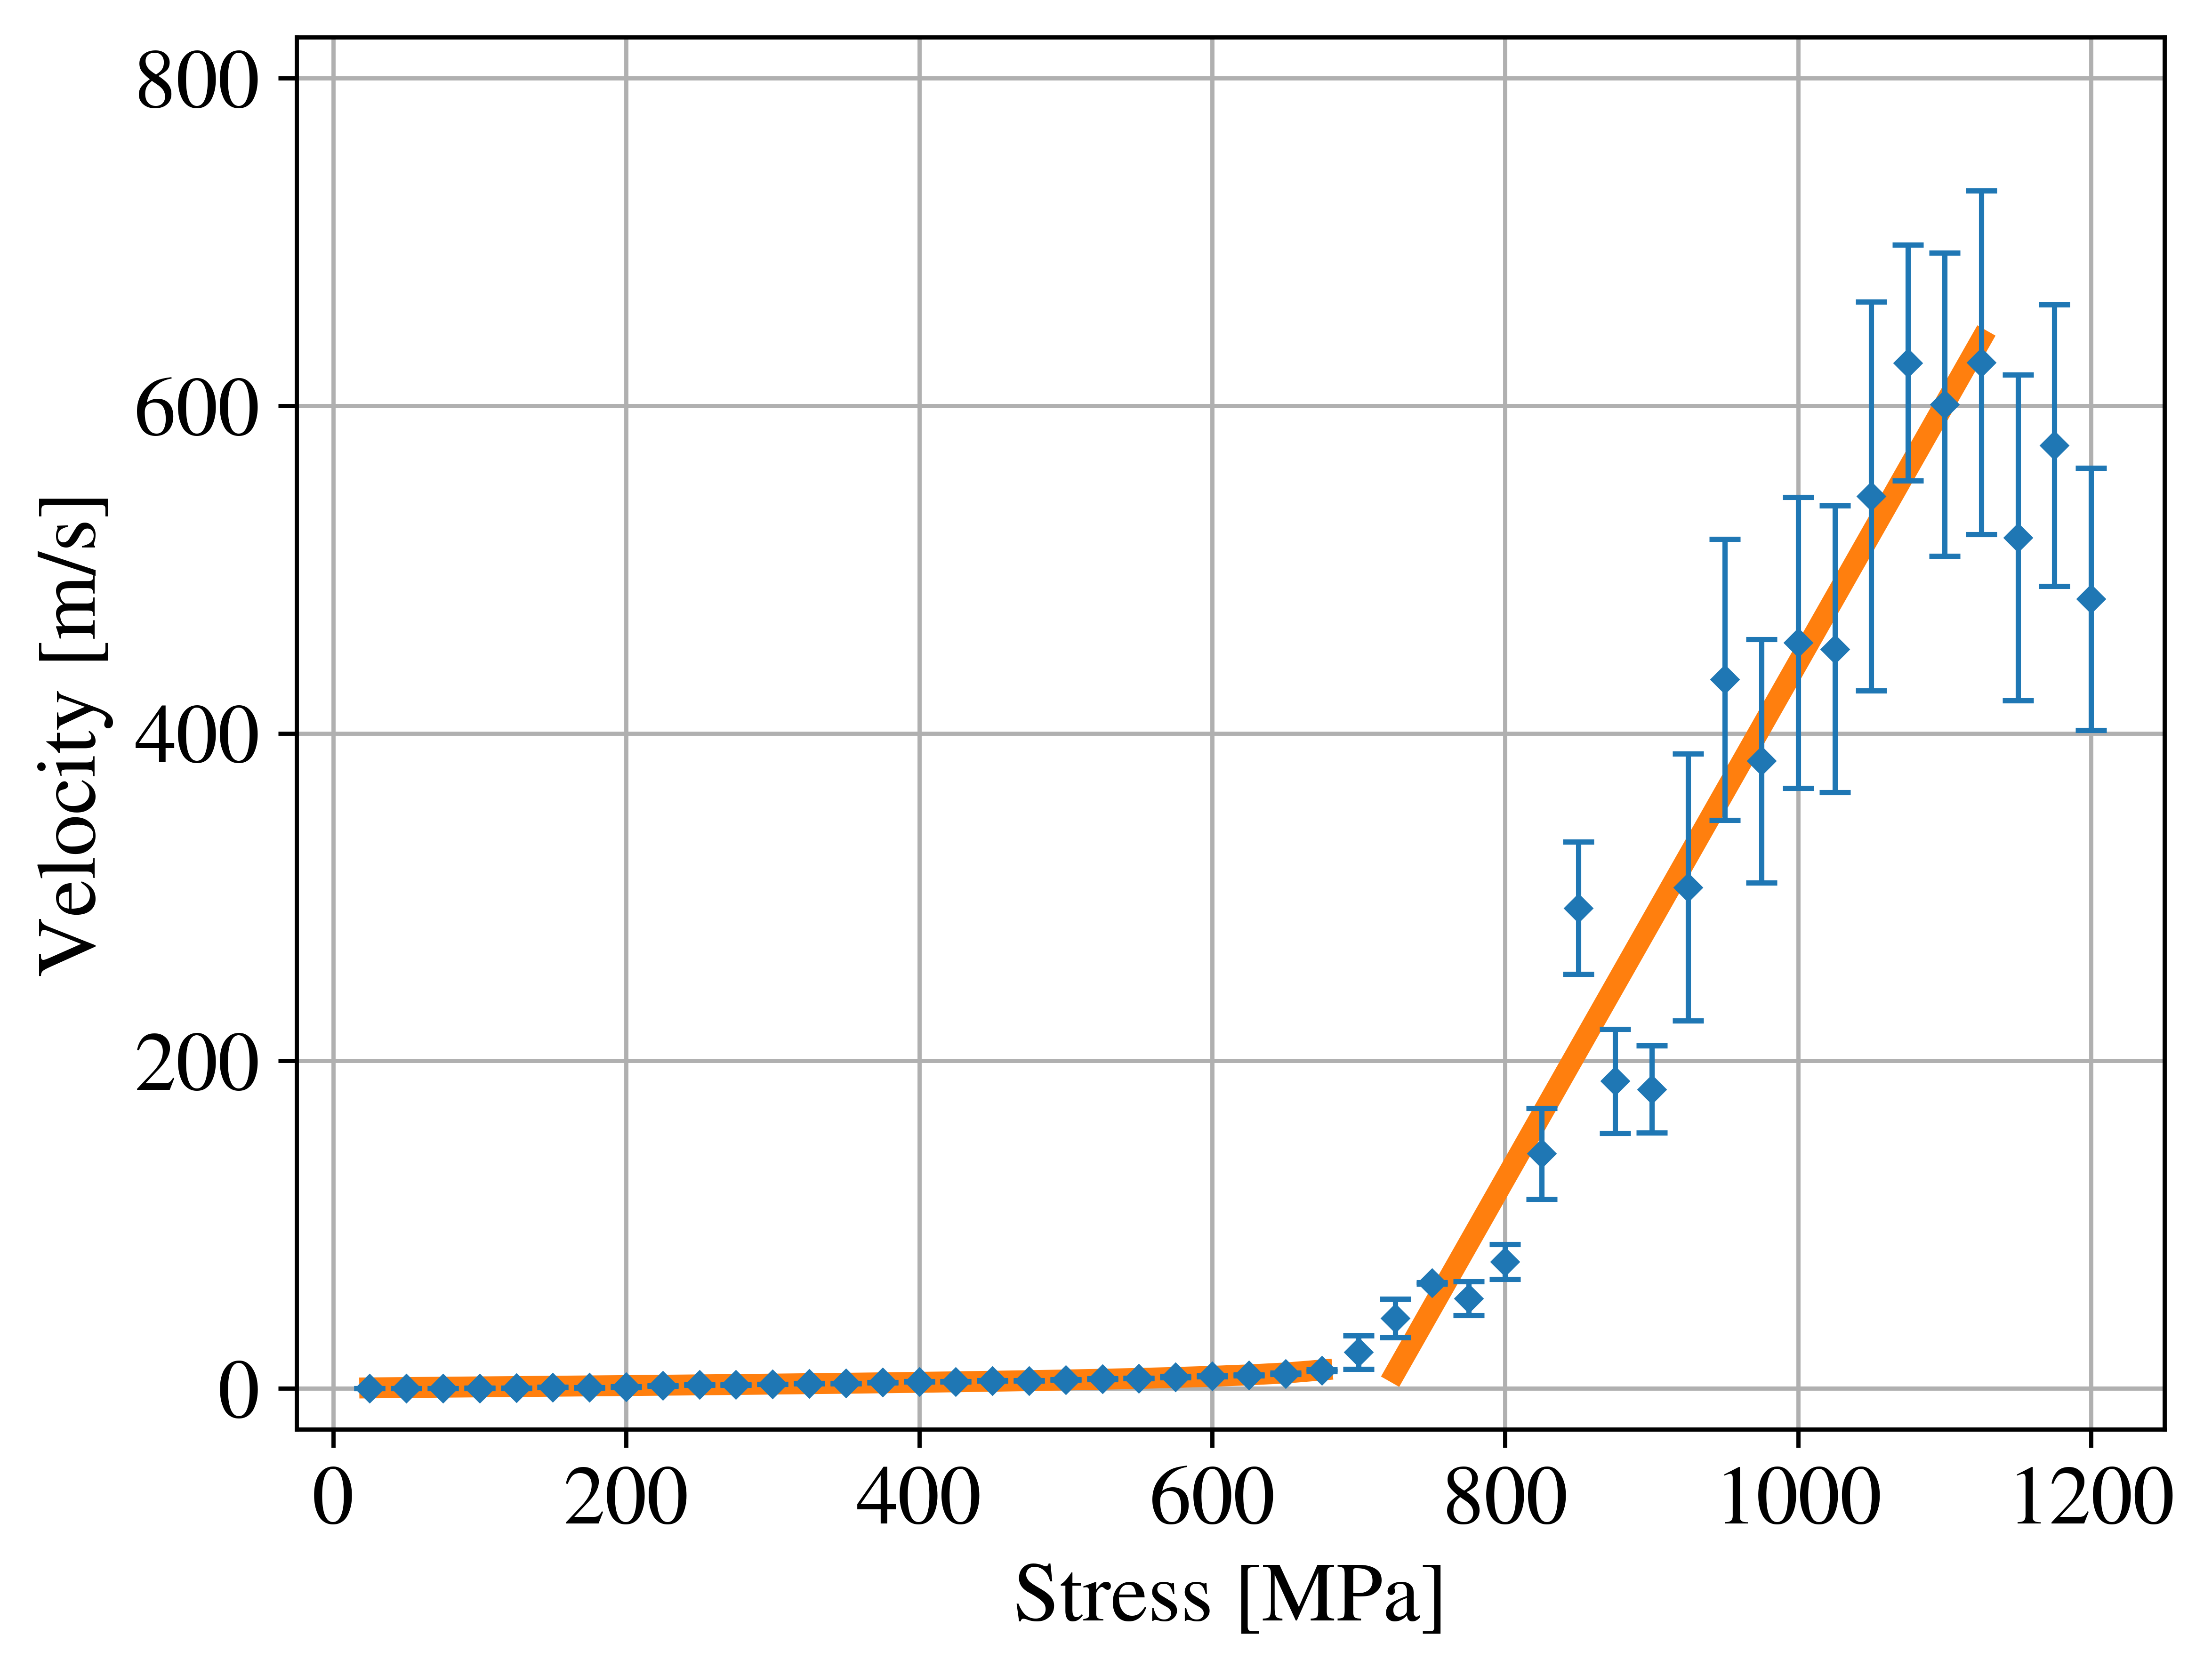
\includegraphics[width=0.48\textwidth]{ScrewMob1.png}}
\hfill
\subfloat[]{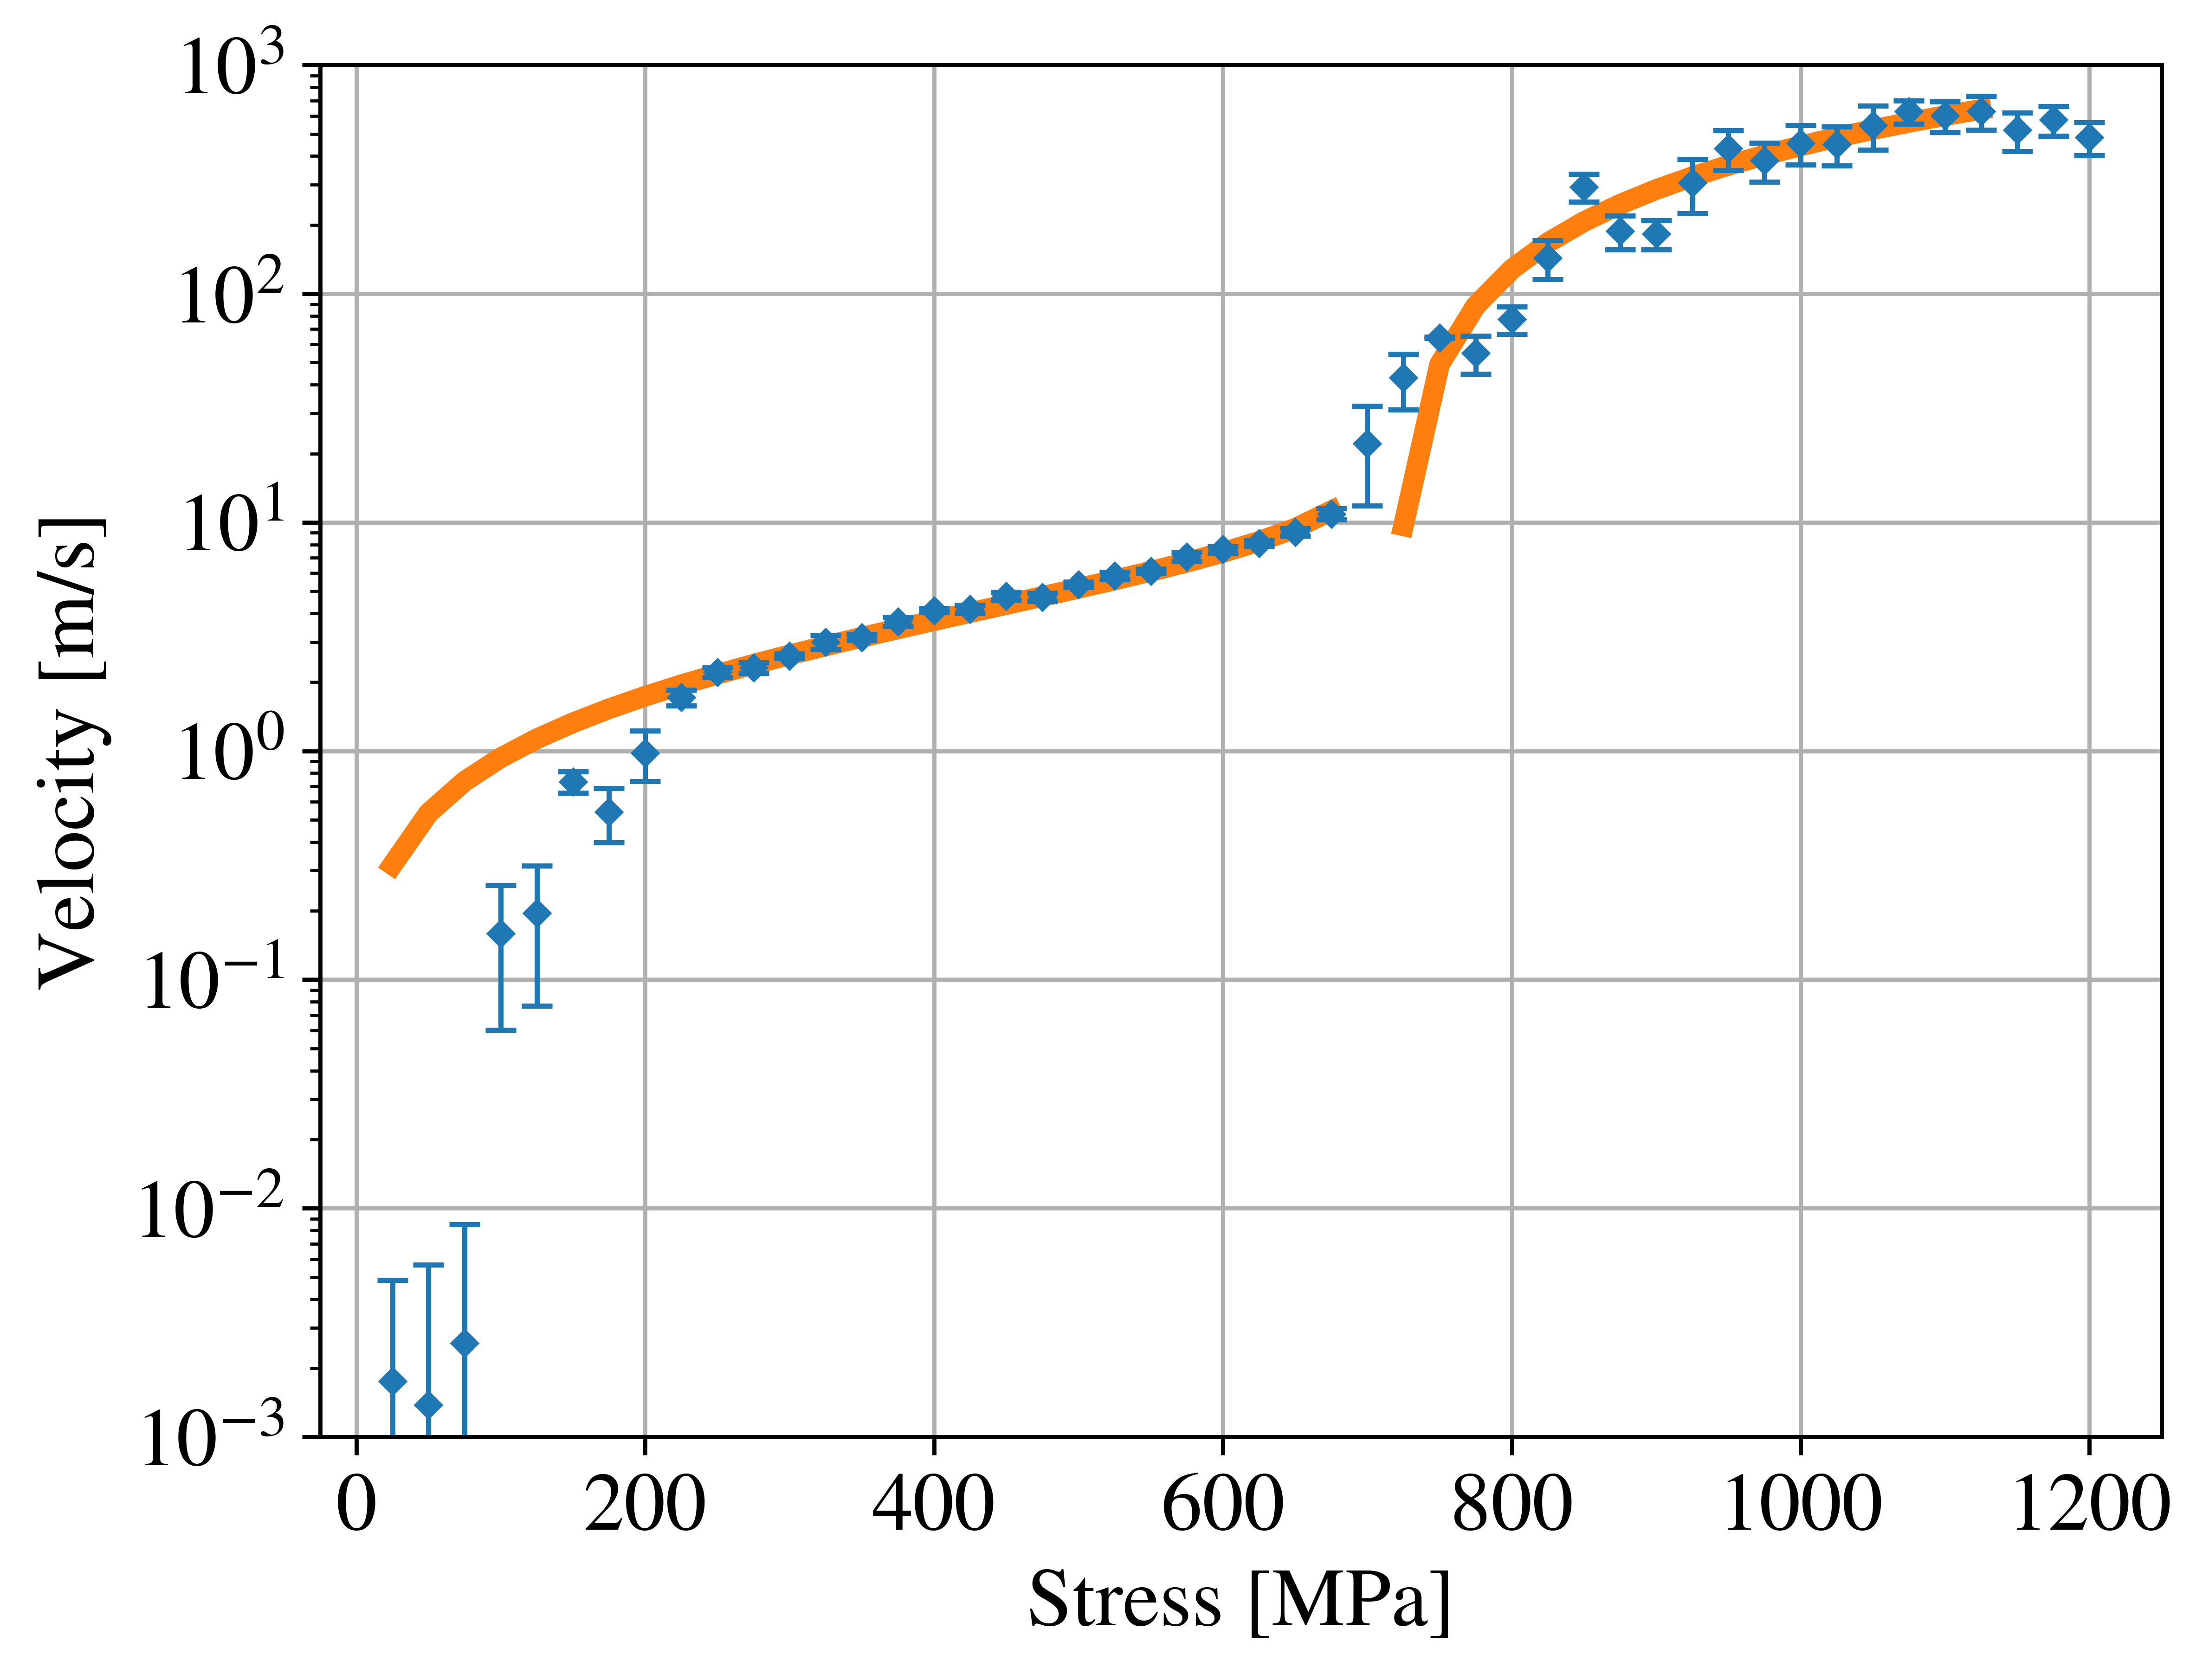
\includegraphics[width=0.48\textwidth]{ScrewMob2.png}}
}

\caption{The variation in the average screw dislocation velocity in UN with shear stress (\textbf{a}) on a linear scale, and~(\textbf{b}) on a semi-log scale. The~error bars represent one standard deviation, and~the orange lines represent piecewise curve~fits.}
\label{Fig:DislocPosTimeScrew}
\end{figure}
%\unskip

\subsubsection{Yield Stress~Estimate}

Based on the definition of the threshold Schmid stress (also known as the critical resolved shear stress (CRSS)), $\tau_S$, as~the stress at which the dislocation moves with a velocity of at least 1 m/s~\cite{Murty2013}, it is found that for the edge dislocation in UN, $\tau_S$ = 179 MPa, whereas for the screw dislocation, $\tau_S$ = 197 MPa. Although~this definition of the CRSS is based on studies on FCC and HCP metals, we assume its validity for UN. According to Stoller and Zinkle~\cite{Stoller2000}, an~upper-limit estimate of the uniaxial yield stress of a polycrystal can be calculated from
\begin{equation}
\sigma_y = 3.06 \tau_S
\label{Eq:Taylor}
\end{equation}
which gives $\sigma_y$ = 548--603 MPa. Unlike the GPa-range yield stresses calculated earlier, which are only valid for single-crystal UN, $\sigma_y$ = 548--603 MPa is comparable to the yield stress of macroscopic samples at room temperatures. However, to~the best of our knowledge, no experimental stress--strain measurements of UN exist in the open~literature.

Another estimate of the yield stress for macroscopic polycrystalline UN can be calculated using the model of Hayes~et~al. \cite{Hayes2004}, which has been used to give a good prediction of the yield stress of $\alpha$-U~\cite{Taylor2008}. This model applies the crack formation criterion of brittle fracture~\cite{Murty2013} to obtain a value of the critical stress at which the elastic strain energy imposed upon an elongated single crystal exceeds the surface energy of the crystal. This critical stress correlates with the yield stress because, although~UN will fail plastically, its brittle fracture provides a guide to the stress at which the elastic limit is reached. For~UN, this critical stress can be calculated as~\cite{Hayes2004, Taylor2008}
\begin{equation}
\sigma_c = 2 \sqrt{\gamma C_{11} / w} 
\end{equation}
where $\gamma$ is the (001) surface energy, $w$ is the sample width, and~$C_{11}$ is the elastic constant. According to the DFT study of Bocharov~et~al. \cite{Bocharov2013}, the~(001) surface energy is 1.44 J/m$^2$. The~sample width, $w$, can be estimated as the size of a 10 $\mu$m single crystal~\cite{Hayes2004, Taylor2008}, which is a typical average grain size. The~value of $C_{11}$ = 423.9 GPa is taken from experiments~\cite{Salleh1986}. Using these values, $\sigma_c$ is about 494 MPa, which agrees within 10\% with the lower limit of the range calculated earlier (i.e., 548 MPa) using \cref{Eq:Taylor}, which is a good agreement considering the widely different approaches used to arrive at the two values. Based on this simple analysis, a~rough estimate of the yield stress of UN can be given as 550~MPa.

\section{Discussion}

In this work, we demonstrated that MD simulations can provide accurate predictions of the nanoindentation hardness of UN. We believe this method can be extended to other nuclear fuels, particularly in high-temperature regimes, where oxidation layers may limit experimental nanoindentation measurements. The~key requirement for an interatomic potential in such simulations is the accurate prediction of the elastic properties and softening behavior. Our findings show that the Kocevski potential gives excellent predictions for nanoindentation hardness, despite its limitations in modeling plasticity dynamics in UN. This is acceptable for simulations where brittle failure dominates, as~the plastic deformation dynamics become less relevant. Our earlier work~\cite{AbdulHameed2024} has further shown that the Kocevski potential provides a reasonable description of elastic behavior, which is the focus in such brittle~regimes.

The Kocevski and Tseplyaev potentials yield different predictions for the principal slip systems in UN. The~Kocevski potential predicts that the principal slip system is $\frac{1}{2} \langle 110 \rangle \{110\}$, based on screw dislocation studies, while the Tseplyaev potential suggests $\frac{1}{2} \langle 110 \rangle \{111\}$, as~derived from edge dislocation studies. Experimental data~\cite{Sole1968} on deformation in UN indicates that the $\{110\}$ planes are the principal slip planes, which aligns with the predictions of the Kocevski potential. This study also noted that screw dislocations are more prevalent in UN~\cite{Sole1968}. This experimental observation combined with our finding---that screw dislocations exhibit larger linear mobility and smaller transition stress to the phonon-drag regime compared to edge dislocations---leads us to recommend the screw dislocation mobility function for use in discrete dislocation dynamics (DDD) simulations of~UN.

The discrepancy in the predictions of the two potentials may arise from the fact that the Tseplyaev potential likely overestimates the covalent nature of bonding in UN. Another explanation for the differing predictions is that the dominant slip planes in UN may vary with temperature, a~phenomenon observed in other materials such as Sr-doped KCl~\cite{Haasen1985}. For~instance, while $\{111\}$ planes are the primary slip planes in UC, this conclusion is based on high-temperature measurements (1680--2200 K) \cite{Vasudevamurthy2022}. Since our simulations are conducted at 300 K, further experimental and DFT studies are required to clarify the principal slip systems in both UN and UC across a range of~temperatures.

Dislocation properties, both static and dynamic, are highly sensitive to the chosen interatomic potential. Thus, quantitative conclusions drawn from atomistic models should be considered approximations~\cite{Puls1976, Liu2012}. For~instance, the~Peierls stress of UN, calculated as 2.98 GPa, aligns with the order of magnitude reported for \ce{UO2} by Skelton and Walker, which ranged from 2.7 to 12.9 GPa depending on the interatomic potential used~\cite{Skelton2017}. Based on preliminary testing %MDPI: “Data not shown” should be avoided. Please cite as a reference/Supplementary Materials or please remove this phrase. %BB: phrase has been removed and sentence rephrased
, we found that the Peierls stress decreases by approximately 1 GPa when the dislocation line length increases from 40 \AA\ to 80 \AA, though~this change does not affect the relative ordering of Peierls stress across the $\frac{1}{2}\langle110\rangle$ slip planes for the edge dislocation. To~ensure comparability, it is crucial to evaluate Peierls stress values under consistent simulation conditions, including the same potential, supercell size, and~strain~rate.

This work presents the first complete mobility functions for $\frac{1}{2}\langle110\rangle$ edge and screw dislocations in UN, providing a foundational step toward parameterizing plasticity dynamics in this material. One limitation of our model is that it is based on simulations at a single temperature (300 K). Key parameters, such as transition stresses and velocities between different regimes, as~well as the phonon drag coefficient, are known to vary strongly with temperature~\cite{Olmsted2005, Gilbert2011}. For~example, transition stresses and velocities between \mbox{regimes I and II} tend to decrease with increasing temperature, while the phonon drag coefficient typically exhibits an inverse temperature dependence ($B$$\sim$$1/T$). Therefore, future work should involve extending these simulations to higher temperatures to analyze the trends in these parameters. Additionally, our atomistic simulations neglect dislocation--dislocation interactions, meaning the mobility function we present here represents an upper limit at 300 K. However, since the Tseplyaev potential treats UN plasticity as that of a purely covalent material, it may underestimate dislocation mobility, leading to a partial cancellation of errors between these two factors. Thus, the~edge dislocation mobility function presented here is expected to be a reasonable~estimate. 

% It should also be noted that the dislocation mobility functions we derived are not continuous at the transition stress. For numerical implementation in a DDD code, both the mobility function and its first derivative must be continuous. This can be achieved by performing ``curve stitching'' between the piecewise functions to ensure smoothness, a task left for future studies. Open-source DDD codes, such as ParaDiS~\cite{Arsenlis2007}, can be extended to incorporate complex mobility functions like those presented here. For instance, Starikov and Tseplyaev~\cite{Starikov2020} implemented a custom mobility function for molybdenum. Such an extension could be similarly implemented for UN using the mobility functions developed in this work.

The estimated threshold Schmid stress for dislocation glide in UN (179--197 MPa) and the corresponding uniaxial yield stress (548--603 MPa) represent upper-limit estimates. This is primarily due to our use of the Taylor factor (3.06) in calculating these values, which could be lower in real materials due to factors such as texture~\cite{Stoller2000}. Nevertheless, the~yield stress predicted by our crack formation criterion (494 MPa) lends confidence to our estimates. An~average yield stress of approximately 550 MPa is reasonable based on our findings, and~we recommend its use as an input parameter in future plasticity or dislocation dynamics models until experimental data are~available.

\section{Conclusions}

In this study, we employed MD simulations to investigate specific aspects of the mechanical behavior of UN. First, we analyzed the deformation behavior in nanometer-sized UN single-crystals. The~Kocevski potential predicted the principal slip system as $\frac{1}{2} \langle 110 \rangle \{110\}$, aligning with experimental data, while the Tseplyaev potential predicted slip on $\frac{1}{2} \langle 110 \rangle \{111\}$. The~study demonstrates that MD simulations of stress--strain curves in single crystals with free surfaces yield accurate estimates of the nanoindentation hardness of UN. Nanoindentation hardness was accurately predicted by the Kocevski potential, though~it struggled to model dynamic plasticity. This methodology is particularly advantageous at elevated temperatures, where oxidation hinders direct measurements of UN's nanoindentation hardness. Further exploration involved the determination of the Peierls stress for the $\frac{1}{2} \langle 110 \rangle$ edge dislocation along the $\{ 110 \}$, $\{ 111 \}$, and~$\{ 112 \}$ slip planes and for the $\frac{1}{2} \langle 110 \rangle$ screw dislocation along $\{110\}$. The~$\{ 111 \}$ plane displayed the smallest value (2.98 GPa), agreeing with the results of the stress--strain behavior predicted by the Tseplyaev potential. For~the screw dislocation, the~Peierls stress is determined to be about 790 MPa using the Kocevski potential. Both edge and screw dislocations are found to move via the kink-pair nucleation mechanism before displaying a linear variation in their velocity with stress. Based on these results, complete dislocation mobility functions were fitted and the linear mobility was found to be 817 $\mathrm{Pa}^{-1} \! \cdot \! \mathrm{s}^{-1}$ for the edge dislocation using the Tseplyaev potential, and~4546 $\mathrm{Pa}^{-1} \! \cdot \! \mathrm{s}^{-1}$ for the screw dislocation using the Kocevski potential. The~threshold Schmid stress was estimated to be between 179 and 197 MPa, corresponding to an upper-limit uniaxial yield stress of 548--603 MPa for polycrystalline UN. These values show the expected orders of magnitude and can be used as inputs for plasticity or dislocation dynamics models. Finally, we observed that, at~intermediate stresses, the~subsonic steady-state motion of the edge dislocation in UN can be interrupted by jumps that have a maximum velocity equal to the average sound~velocity.

To the best of our knowledge, this study is the first computational investigation of the stress--strain behavior and dislocation properties in UN, and~the first that attempts to fit complete mobility functions for dislocations in a nuclear fuel. We believe this work provides a baseline for the computational study of dislocations in nuclear fuels that can be expanded and built upon by, e.g.,~conducting the analysis at higher temperatures, which are more relevant for the operational conditions of nuclear~reactors.


%%%%%%%%%%%%%%%%%%%%%%%%%%%%%%%%%%%%%%%%%%

\vspace{6pt}

\authorcontributions{Conceptualization, M.A., B.B., and A.C.; methodology, M.A.; formal analysis, M.A.; writing---original draft preparation, M.A.; writing---review and editing, M.A., B.B., and A.C.; visualization, M.A.; project administration, B.B. and A.C.; funding acquisition, A.C. All authors have read and agreed to the published version of the~manuscript.}

\funding{This %MDPI: Information regarding the funder and the funding number should be provided. Please check the accuracy of funding data and any other information carefully. %BB: this is accurate. there is no funding 'number'
 research was funded by the Westinghouse Electric~Company.  This research made use of the resources of the High-Performance Computing Center at Idaho National Laboratory, which is supported by the Office of Nuclear Energy of the U.S. Department of Energy and the Nuclear Science User Facilities under Contract No. DE-AC07-05ID14517.}

\institutionalreview{\hl{~} %MDPI: In this section, you should add the Institutional Review Board Statement and approval number, if relevant to your study. You might choose to exclude this statement if the study did not require ethical approval. Please note that the Editorial Office might ask you for further information. Please add “The study was conducted in accordance with the Declaration of Helsinki, and approved by the Institutional Review Board (or Ethics Committee) of NAME OF INSTITUTE (protocol code XXX and date of approval).” for studies involving humans. OR “The animal study protocol was approved by the Institutional Review Board (or Ethics Committee) of NAME OF INSTITUTE (protocol code XXX and date of approval).” for studies involving animals. OR “Ethical review and approval were waived for this study due to REASON (please provide a detailed justification).” OR “Not applicable” for studies not involving humans or animals. %BB: not relevant
}

\informedconsent{\hl{~} %MDPI: Any research article describing a study involving humans should contain this statement. Please add ``Informed consent was obtained from all subjects involved in the study.'' OR ``Patient consent was waived due to REASON (please provide a detailed justification).'' OR ``Not applicable'' for studies not involving humans. You might also choose to exclude this statement if the study did not involve humans. %BB: not relevant

%Written informed consent for publication must be obtained from participating patients who can be identified (including by the patients themselves). Please state ``Written informed consent has been obtained from the patient(s) to publish this paper'' if applicable. %BB: not relevant
}

\dataavailability{\hl{The raw data supporting the conclusions of this article will be made available by the authors on request.}} %MDPI: Data Availability Statements provide details regarding where data supporting reported results can be found, including links to publicly archived datasets analyzed or generated during the study.
%Below are suggested Data Availability Statements:
%1. Data available in a publicly accessible repository
%  -The data presented in this study are openly available in [repository name e.g., FigShare] at [doi], reference number [reference number].
%2. Data available in a publicly accessible repository that does not issue DOIs
%  -Publicly available datasets were analyzed in this study. This data can be found here: [link/accession number].
%3. Data available on request due to restrictions eg privacy or ethical
%  -The data presented in this study are available on request from the corresponding author. The data are not publicly available due to [insert reason here].
%(Reason is necessary)
%4. 3rd Party Data
%  -Restrictions apply to the availability of these data. Data was obtained from [third party] and are available [from the authors/at URL] with the permission of [third party].
%5. Data is contained within the article or supplementary material
%  -The data presented in this study are available in [insert article or supplementary material here].
%6. The raw data supporting the conclusions of this article will be made available by the authors on request.
%BB: statement #6 is utilized
 

\acknowledgments{\hl{The} %MDPI: Please ensure that all individuals included in this section have consented to the acknowledgement.
 authors would like to thank Michael W. D. Cooper, Conor O. T. Galvin, \mbox{Mahmoud} Hawary, and Shehab Shousha for the fruitful discussions and useful suggestions. %MDPI: Please consider if this statement belongs to Funding section. %BB: This statement has been moved from acknowledgments to the funding section. 
 Mohamed AbdulHameed dedicates this work to the memory of Ammar~Alkhowesky.}

\conflictsofinterest{\hl{Author Antoine Claisse was employed by the company Westinghouse Electric Sweden. The remaining authors declare that the research was conducted in the absence of any commercial or financial relationships that could be construed as a potential conflict of interest.}} %MDPI: 1. For commercial affiliations, all authors must be accounted for. We recommend using the following template:
%Template:
%Author XXXXXXX was employed by the company XXXXXXX.
%The remaining authors declare that the research was conducted in the absence of any commercial or financial relationships that could be construed as a potential conflict of interest
%BB: confirmed
 


%%%%%%%%%%%%%%%%%%%%%%%%%%%%%%%%%%%%%%%%%%

\begin{adjustwidth}{-\extralength}{0cm}

\reftitle{References}

\begin{thebibliography}{999}

\bibitem[Ekberg et~al.(2018)Ekberg, Costa, Hedberg, and Jolkkonen]{Ekberg2018}
\hl{Ekberg, C.; Costa, D.R.; Hedberg, M.; Jolkkonen, M.} %MDPI: Please DO NOT delete or add any reference during proofreading stage since paper has been accepted. %BB: confirmed
\newblock Nitride fuel for {Gen} {IV} nuclear power systems.
\newblock {\em J. Radioanal. Nucl. Chem.} {\bf 2018},
  {\em 318},~1713--1725.
\newblock {\url{https://doi.org/10.1007/s10967-018-6316-0}}.

\bibitem[Wallenius(2020)]{Wallenius2020}
Wallenius, J.
\newblock Nitride fuels.
\newblock {\em Compr. Nucl. Mater.} {\bf 2020}, {\em 5},~88--101.
\newblock {\url{https://doi.org/10.1016/B978-0-12-803581-8.11694-7}}.

\bibitem[Uno et~al.(2020)Uno, Nishi, and Takano]{Uno2020}
Uno, M.; Nishi, T.; Takano, M.
\newblock Thermodynamic and thermophysical properties of the actinide nitrides.
\newblock In {\em Comprehensive Nuclear Materials}, 2nd ed.; \hl{Elsevier: Amsterdam, The Netherlands}%MDPI: Please confirm newly added information, including the following highlights. %BB: confirmed
, 2020; \textls[-15]{pp. 202--231. {\url{https://doi.org/10.1016/B978-0-12-803581-8.11749-7}}}.

\bibitem[Olander and Motta(2017)]{Olander2017}
Olander, D.R.; Motta, A.T.
\newblock Fundamentals. In {\em Light Water Reactor Materials}; American
  Nuclear Society: \hl{Westmont, IL, USA}, 2017; Volume 1.

\bibitem[Olander and Motta(2021)]{Olander2021}
Olander, D.R.; Motta, A.T.
\newblock Applications. In {\em Light Water Reactor Materials}; American
  Nuclear Society: \hl{Westmont, IL, USA}, 2021; Volume 2.

\bibitem[Ivashchenko et~al.(2007)Ivashchenko, Turchi, and
  Shevchenko]{Ivashchenko2007}
Ivashchenko, V.I.; Turchi, P.E.; Shevchenko, V.I.
\newblock Simulations of the mechanical properties of crystalline,
  nanocrystalline, and amorphous {SiC} and {Si}.
\newblock {\em Phys. Rev. B-Condens. Matter Mater. Phys.} {\bf
  2007}, {\em 75}, \hl{085209}.
\newblock {\url{https://doi.org/10.1103/PhysRevB.75.085209}}.

\bibitem[Li et~al.(2020)Li, Gao, Zhan, Fang, and Zhang]{Li2020}
Li, Z.; Gao, Y.; Zhan, S.; Fang, H.; Zhang, Z.
\newblock Molecular dynamics study on temperature and strain rate dependences
  of mechanical properties of single crystal {Al} under uniaxial loading.
\newblock {\em AIP Adv.} {\bf 2020}, {\em 10}, \hl{075321}.
\newblock {\url{https://doi.org/10.1063/1.5086903}}.

\bibitem[Hansson et~al.(2022)Hansson, Ahadi, and Melin]{Hansson2022}
Hansson, P.; Ahadi, A.; Melin, S.
\newblock Molecular dynamic modelling of the combined influence from strain
  rate and temperature at tensile loading of nanosized single crystal {Cu}
  beams.
\newblock {\em Mater. Today Commun.} {\bf 2022}, {\em 31}, \hl{103277}.
\newblock {\url{https://doi.org/10.1016/j.mtcomm.2022.103277}}.

\bibitem[Sole and Walt(1968)]{Sole1968}
Sole, M.J.; Walt, C.M.V.D.
\newblock Oxidation and deformation studies of uranium nitride by electron
  microscopy.
\newblock {\em Acta Metall.} {\bf 1968}, {\em 16}, \hl{501--510}.
\newblock {\url{https://doi.org/10.1016/0001-6160(68)90124-7}}.

\bibitem[Xiu et~al.(2021)Xiu, Jin, Bawane, Tyburska-Püschel, Jaques, Field,
  Giglio, and He]{Xiu2021}
Xiu, P.; Jin, M.; Bawane, K.; Tyburska-Püschel, B.; Jaques, B.J.; Field, K.G.;
  Giglio, J.J.; He, L.
\newblock Dislocation Loops in Proton Irradiated Uranium-Nitrogen-Oxygen
  System.
\newblock {\em J. Nucl. Mater.} {\bf 2021}, {\em 557}, \hl{153244}.
\newblock {\url{https://doi.org/10.1016/j.jnucmat.2021.153244}}.

\bibitem[Tseplyaev and Starikov(2016)]{Tseplyaev2016}
Tseplyaev, V.I.; Starikov, S.V.
\newblock The atomistic simulation of pressure-induced phase transition in
  uranium mononitride.
\newblock {\em J. Nucl. Mater.} {\bf 2016}, {\em 480},~7--14.
\newblock {\url{https://doi.org/10.1016/j.jnucmat.2016.07.048}}.

\bibitem[AbdulHameed et~al.(2024)AbdulHameed, Beeler, Galvin, and
  Cooper]{AbdulHameed2024}
AbdulHameed, M.; Beeler, B.; Galvin, C.O.; Cooper, M.W.
\newblock Assessment of uranium nitride interatomic potentials.
\newblock {\em J. Nucl. Mater.} {\bf 2024}, \emph{\hl{600}}, 155247.
\newblock
  {\url{https://doi.org/https://doi.org/10.1016/j.jnucmat.2024.155247}}.

\bibitem[Skelton and Walker(2017)]{Skelton2017}
Skelton, R.; Walker, A.M.
\newblock {Peierls-Nabarro} modeling of dislocations in {UO$_2$}.
\newblock {\em J. Nucl. Mater.} {\bf 2017}, {\em 495}, \hl{202--210}.
\newblock {\url{https://doi.org/10.1016/j.jnucmat.2017.08.024}}.

\bibitem[Osetsky and Bacon(2003)]{Osetsky2003}
Osetsky, Y.N.; Bacon, D.J.
\newblock An atomic-level model for studying the dynamics of edge dislocations
  in metals.
\newblock {\em Model. Simul. Mater. Sci. Eng.}
  {\bf 2003}, {\em 11}, \hl{427}.
\newblock {\url{https://doi.org/10.1088/0965-0393/11/4/302}}.

\bibitem[Liu et~al.(2012)Liu, Wu, Wang, Feng, and Wu]{Liu2012}
Liu, L.; Wu, X.Z.; Wang, R.; Feng, H.F.; Wu, S.
\newblock On the generalized stacking energy, core structure and {Peierls}
  stress of the $\frac{1}{2} \langle 110 \rangle \{110\}$ dislocations in
  alkali halides.
\newblock {\em Eur. Phys. J. B} {\bf 2012}, {\em 85}, \hl{58}.
\newblock {\url{https://doi.org/10.1140/epjb/e2011-20767-7}}.

\bibitem[Cho et~al.(2017)Cho, Molinari, and Anciaux]{Cho2017}
Cho, J.; Molinari, J.F.; Anciaux, G.
\newblock Mobility law of dislocations with several character angles and
  temperatures in {FCC} aluminum.
\newblock {\em Int. J. Plast.} {\bf 2017}, {\em 90}, \hl{66--75}.
\newblock {\url{https://doi.org/10.1016/j.ijplas.2016.12.004}}.

\bibitem[Dang et~al.(2019)Dang, Bamney, Bootsita, Capolungo, and
  Spearot]{Dang2019}
Dang, K.; Bamney, D.; Bootsita, K.; Capolungo, L.; Spearot, D.E.
\newblock Mobility of dislocations in aluminum: Faceting and asymmetry during
  nanoscale dislocation shear loop expansion.
\newblock {\em Acta Mater.} {\bf 2019}, {\em 168}, \hl{426--435}.
\newblock {\url{https://doi.org/10.1016/j.actamat.2019.02.034}}.

\bibitem[Olmsted et~al.(2005)Olmsted, Hector, Curtin, and Clifton]{Olmsted2005}
Olmsted, D.L.; Hector, L.G.; Curtin, W.A.; Clifton, R.J.
\newblock Atomistic simulations of dislocation mobility in {Al}, {Ni} and
  {Al/Mg} alloys.
\newblock {\em Model. Simul. Mater. Sci. Eng.}
  {\bf 2005}, {\em 13}, \hl{371}.
\newblock {\url{https://doi.org/10.1088/0965-0393/13/3/007}}.

\bibitem[Kaloni et~al.(2023)Kaloni, Prudil, Spearot, and Torres]{Kaloni2023}
Kaloni, T.P.; Prudil, A.; Spearot, D.E.; Torres, E.
\newblock Modeling of dislocation properties in {Fe$_{40}$Cr$_{25}$Ni$_{35}$}
  and {Fe$_{50}$Cr$_{20}$Ni$_{30}$} systems.
\newblock {\em Nucl. Eng. Des.} {\bf 2023}, {\em 411}, \hl{112422}.
\newblock {\url{https://doi.org/10.1016/j.nucengdes.2023.112422}}.

\bibitem[Yadav et~al.(2014)Yadav, Ramprasad, Misra, and Liu]{Yadav2014}
Yadav, S.K.; Ramprasad, R.; Misra, A.; Liu, X.Y.
\newblock Core structure and {Peierls} stress of edge and screw dislocations in
  {TiN}: A density functional theory study.
\newblock {\em Acta Mater.} {\bf 2014}, {\em 74}, \hl{268--277}.
\newblock {\url{https://doi.org/10.1016/j.actamat.2014.04.047}}.

\bibitem[Ukita et~al.(2018)Ukita, Nakamura, Yokoi, and Matsunaga]{Ukita2018}
Ukita, M.; Nakamura, A.; Yokoi, T.; Matsunaga, K.
\newblock Electronic and atomic structures of edge and screw dislocations in
  rock salt structured ionic crystals.
\newblock {\em Philos. Mag.} {\bf 2018}, {\em 98}, \hl{2189--2204}.
\newblock {\url{https://doi.org/10.1080/14786435.2018.1478146}}.

\bibitem[Kocevski et~al.(2022)Kocevski, Cooper, Claisse, and
  Andersson]{Kocevski2022II}
Kocevski, V.; Cooper, M.W.; Claisse, A.J.; Andersson, D.A.
\newblock Development and application of a uranium mononitride ({UN})
  potential: Thermomechanical properties and {Xe} diffusion.
\newblock {\em J. Nucl. Mater.} {\bf 2022}, {\em 562}, \hl{153553}.
\newblock {\url{https://doi.org/10.1016/j.jnucmat.2022.153553}}.

\bibitem[Thompson et~al.(2022)Thompson, Aktulga, Berger, Bolintineanu, Brown,
  Crozier, in~'t Veld, Kohlmeyer, Moore, Nguyen, Shan, Stevens, Tranchida,
  Trott, and Plimpton]{Thompson2022}
Thompson, A.P.; Aktulga, H.M.; Berger, R.; Bolintineanu, D.S.; Brown, W.M.;
  Crozier, P.S.; in~'t Veld, P.J.; Kohlmeyer, A.; Moore, S.G.; Nguyen, T.D.;
  et~al.
\newblock {LAMMPS}---A flexible simulation tool for particle-based materials
  modeling at the atomic, meso, and continuum scales.
\newblock {\em Comput. Phys. Commun.} {\bf 2022}, {\em 271}, \hl{108171}.
\newblock {\url{https://doi.org/10.1016/j.cpc.2021.108171}}.

\bibitem[Stukowski(2010)]{Stukowski2010}
Stukowski, A.
\newblock Visualization and analysis of atomistic simulation data with
  {OVITO}---The Open Visualization Tool.
\newblock {\em Model. Simul. Mater. Sci. Eng.}
  {\bf 2010}, {\em 18}, \hl{015012}.
\newblock {\url{https://doi.org/10.1088/0965-0393/18/1/015012}}.

\bibitem[Lao et~al.(2013)Lao, Tam, Pinisetty, and Gupta]{Lao2013}
Lao, J.; Tam, M.N.; Pinisetty, D.; Gupta, N.
\newblock Molecular dynamics simulation of {FCC} metallic nanowires: A review.
\newblock {\em  J. Miner. Met. Mater. Soc.}
  {\bf 2013}, {\em 65}, \hl{175--184}.
\newblock {\url{https://doi.org/10.1007/s11837-012-0465-3}}.

\bibitem[Rösler et~al.(2007)Rösler, Harders, and Bäker]{Rosler2007}
Rösler, J.; Harders, H.; Bäker, M.
\newblock {\em Mechanical Behaviour of Engineering Materials}; Springer:  \hl{Berlin/Heidelberg, Germany},  2007.

\bibitem[Larsen(2020)]{Larsen2020}
Larsen, P.M.
\newblock Revisiting the Common Neighbour Analysis and the Centrosymmetry
  Parameter. \emph{arXiv} \textbf{2020}, arXiv:2003.08879. \url{https://doi.org/10.48550/arXiv.2003.08879}.

\bibitem[Kelchner and Plimpton(1998)]{Kelchner1998}
Kelchner, C.L.; Plimpton, S.
\newblock Dislocation nucleation and defect structure during surface
  indentation.
\newblock {\em Phys. Rev. B-Condens. Matter Mater. Phys.} {\bf
  1998}, {\em 58}, \hl{11085}.
\newblock {\url{https://doi.org/10.1103/PhysRevB.58.11085}}.

\bibitem[Bulatov and Cai(2006)]{Bulatov2006}
Bulatov, V.; Cai, W.
\newblock {\em Computer Simulations of Dislocations}; Oxford University Press: \hl{Oxford, UK},
  2006.

\bibitem[Stukowski et~al.(2012)Stukowski, Bulatov, and Arsenlis]{Stukowski2012}
Stukowski, A.; Bulatov, V.V.; Arsenlis, A.
\newblock Automated identification and indexing of dislocations in crystal
  interfaces.
\newblock {\em Model. Simul. Mater. Sci. Eng.}
  {\bf 2012}, {\em 20}, \hl{085007}.
\newblock {\url{https://doi.org/10.1088/0965-0393/20/8/085007}}.

\bibitem[Cai and Nix(2016)]{Cai2016}
Cai, W.; Nix, W.
\newblock {\em Imperfections in Crystalline Solids}, 1st ed.; Cambridge
  University Press: \hl{Cambridge, UK}, 2016.
\newblock {\url{https://doi.org/10.1017/cbo9781316389508}}.

\bibitem[Hull and Bacon(2011)]{Hull2011}
Hull, D.; Bacon, D.J.
\newblock {\em Introduction to Dislocations}, 5th ed.; Butterworth-Heinemann: \hl{Oxford, UK},
  2011; pp. 124--126.
\newblock {\url{https://doi.org/10.1016/C2009-0-64358-0}}.

\bibitem[Smoluchowski(1966)]{Smoluchowski1966}
Smoluchowski, R.
\newblock Dislocations in ionic crystals: Structure, charge effects and
  interaction with Impurities.
\newblock {\em J. Phys. Colloq.} {\bf 1966}, {\em 27},~3--11.
\newblock {\url{https://doi.org/10.1051/jphyscol:1966301}}.

\bibitem[Cooper et~al.(2023)Cooper, Rizk, Matthews, Kocevski, Craven, Gibson,
  and Andersson]{Cooper2023}
Cooper, M.W.; Rizk, J.; Matthews, C.; Kocevski, V.; Craven, G.T.; Gibson, T.;
  Andersson, D.A.
\newblock Simulations of self- and {Xe} diffusivity in uranium mononitride
  including chemistry and irradiation effects.
\newblock {\em J. Nucl. Mater.} {\bf 2023}, {\em 587}, \hl{154685}.
\newblock {\url{https://doi.org/10.1016/j.jnucmat.2023.154685}}.

\bibitem[Gilbert et~al.(2011)Gilbert, Queyreau, and Marian]{Gilbert2011}
Gilbert, M.R.; Queyreau, S.; Marian, J.
\newblock Stress and temperature dependence of screw dislocation mobility in
  {$\alpha$-Fe} by molecular dynamics.
\newblock {\em Phys. Rev. B-Condens. Matter Mater. Phys.} {\bf
  2011}, {\em 84}, \hl{174103}.
\newblock {\url{https://doi.org/10.1103/PhysRevB.84.174103}}.

\bibitem[Puls and Norgett(1976)]{Puls1976}
Puls, M.P.; Norgett, M.J.
\newblock Atomistic calculation of the core structure and {Peierls} energy of
  an ($a$/2) [110] edge dislocation in {MgO}.
\newblock {\em J. Appl. Phys.} {\bf 1976}, {\em 47}, \hl{466--477}.
\newblock {\url{https://doi.org/10.1063/1.322670}}.

\bibitem[Starikov and Tseplyaev(2020)]{Starikov2020}
Starikov, S.; Tseplyaev, V.
\newblock Two-scale simulation of plasticity in molybdenum: Combination of
  atomistic simulation and dislocation dynamics with non-linear mobility
  function.
\newblock {\em Comput. Mater. Sci.} {\bf 2020}, {\em 179}, \hl{109585}.
\newblock {\url{https://doi.org/10.1016/j.commatsci.2020.109585}}.

\bibitem[Ventelon et~al.(2009)Ventelon, Willaime, and Leyronnas]{Ventelon2009}
Ventelon, L.; Willaime, F.; Leyronnas, P.
\newblock Atomistic simulation of single kinks of screw dislocations in
  {$\alpha$-Fe}.
\newblock {\em J. Nucl. Mater.} {\bf 2009}, {\em 386--388}, \hl{26--29}.
\newblock {\url{https://doi.org/10.1016/j.jnucmat.2008.12.053}}.

\bibitem[Kresse and Truskinovsky(2004)]{Kresse2004}
Kresse, O.; Truskinovsky, L.
\newblock Lattice friction for crystalline defects: From dislocations to
  cracks.
\newblock {\em J. Mech. Phys. Solids} {\bf 2004}, {\em
  52}, \hl{2521--2543}.
\newblock {\url{https://doi.org/10.1016/j.jmps.2004.04.011}}.

\bibitem[Salleh et~al.(1986)Salleh, Macdonald, Saunders, and
  de~V~Du~Plessis]{Salleh1986}
Salleh, M.D.; Macdonald, J.E.; Saunders, G.A.; Du Plessis, P.D.V.
\newblock Hydrostatic pressure dependences of elastic constants and vibrational
  anharmonicity of uranium nitride.
\newblock {\em J. Mater. Sci.} {\bf 1986}, {\em 21},~2577--2580.

\bibitem[Wen et~al.(2022)Wen, Tao, Spearot, and Phillpot]{Wen2022}
Wen, P.; Tao, G.; Spearot, D.E.; Phillpot, S.R.
\newblock Molecular dynamics simulation of the shock response of materials: A
  tutorial.
\newblock {\em J. Appl. Phys.} {\bf 2022}, {\em 131}, 051101.
\newblock {\url{https://doi.org/10.1063/5.0076266}}.

\bibitem[Pal and Ray(2020)]{Pal2020}
Pal, S.; Ray, B.C.
\newblock {\em Molecular Dynamics Simulation of Nanostructured Materials: An
  Understanding of Mechanical Behavior}, 1st ed.; CRC Press:  \hl{Boca Raton, FL, USA},  2020.

\bibitem[Adachi et~al.(2009)Adachi, Kurosaki, Uno, Yamanaka, Takano, Akabori,
  and Minato]{Adachi2009}
Adachi, J.; Kurosaki, K.; Uno, M.; Yamanaka, S.; Takano, M.; Akabori, M.;
  Minato, K.
\newblock Mechanical properties at sub-microscale and macroscale of
  polycrystalline uranium mononitride.
\newblock {\em J. Nucl. Mater.} {\bf 2009}, {\em 384},~6--11. \textls[-15]{\url{https://doi.org/10.1016/j.jnucmat.2008.09.019}}.

\bibitem[Frazer et~al.(2021)Frazer, Maiorov, Carvajal-Nuñez, Evans,
  Kardoulaki, Dunwoody, Saleh, and White]{Frazer2021}
Frazer, D.; Maiorov, B.; Carvajal-Nuñez, U.; Evans, J.; Kardoulaki, E.;
  Dunwoody, J.; Saleh, T.A.; White, J.T.
\newblock High temperature mechanical properties of fluorite crystal structured
  materials ({CeO$_2$}, {ThO$_2$}, and {UO$_2$}) and advanced accident tolerant
  fuels ({U$_3$Si$_2$}, {UN}, and {UB$_2$}).
\newblock {\em J. Nucl. Mater.} {\bf 2021}, {\em 554}, \hl{153035}.
\newblock {\url{https://doi.org/10.1016/j.jnucmat.2021.153035}}.

\bibitem[Kuksin et~al.(2016)Kuksin, Starikov, Smirnova, and
  Tseplyaev]{Kuksin2016}
Kuksin, A.Y.; Starikov, S.V.; Smirnova, D.E.; Tseplyaev, V.I.
\newblock The diffusion of point defects in uranium mononitride: Combination of
  {DFT} and atomistic simulation with novel potential.
\newblock {\em J. Alloys Compd.} {\bf 2016}, {\em
  658},~385--394.
\newblock {\url{https://doi.org/10.1016/j.jallcom.2015.10.223}}.

\bibitem[Walt and Sole(1967)]{VanDerWalt1967}
Walt, C.M.V.D.; Sole, M.J.
\newblock On the plastic behaviour of crystals with the {NaCl}-structure.
\newblock {\em Acta Metall.} {\bf 1967}, {\em 15}, \hl{459--462}.
\newblock {\url{https://doi.org/10.1016/0001-6160(67)90076-4}}.

\bibitem[Vasudevamurthy and Nelson(2022)]{Vasudevamurthy2022}
Vasudevamurthy, G.; Nelson, A.T.
\newblock Uranium carbide properties for advanced fuel modeling: A review.
\emph{\hl{J. Nucl. Mater.}} \textbf{2022}, \emph{\hl{558}}, \hl{153145}.
\newblock {\url{https://doi.org/10.1016/j.jnucmat.2021.153145}}.

\bibitem[Haasen(1985)]{Haasen1985}
Haasen, P.
\newblock Dislocations and the plasticity of ionic crystals.
\newblock {\em Mater. Sci. Technol.} {\bf 1985}, {\em 1}, \hl{1013--1024}.
\newblock {\url{https://doi.org/10.1179/mst.1985.1.12.1013}}.

\bibitem[Desai et~al.(2008)Desai, Millett, and Wolf]{Desai2008}
Desai, T.G.; Millett, P.C.; Wolf, D.
\newblock Molecular dynamics study of diffusional creep in nanocrystalline
  {UO$_2$}.
\newblock {\em Acta Mater.} {\bf 2008}, {\em 56}, \hl{4489--4497}.
\newblock {\url{https://doi.org/10.1016/j.actamat.2008.02.052}}.

\bibitem[Taylor(2008)]{Taylor2008}
Taylor, C.D.
\newblock Evaluation of first-principles techniques for obtaining materials
  parameters of $\alpha$-uranium and the (001) $\alpha$-uranium surface.
\newblock {\em Phys. Rev. B-Condens. Matter Mater. Phys.} {\bf
  2008}, {\em 77}, \hl{094119}.
\newblock {\url{https://doi.org/10.1103/PhysRevB.77.094119}}.

\bibitem[Meyers and Chawla(2009)]{Meyers2009}
Meyers, M.; Chawla, K.
\newblock {\em Mechanical Behavior of Materials}, 2nd ed.; Cambridge University Press: \hl{Cambridge, UK}, 2009.

\bibitem[Yu et~al.(2009)Yu, Wang, and Yu]{Yu2009b}
Yu, S.; Wang, C.Y.; Yu, T.
\newblock The kink-pair nucleation in edge dislocation motion.
\newblock {\em Solid State Sci.} {\bf 2009}, {\em 11}, \hl{733--739}.
\newblock {\url{https://doi.org/10.1016/j.solidstatesciences.2008.08.005}}.

\bibitem[Baranov et~al.(2013)Baranov, Devyatko, Tenishev, Khlunov, and
  Khomyakov]{Baranov2013}
Baranov, V.G.; Devyatko, Y.N.; Tenishev, A.V.; Khlunov, A.V.; Khomyakov, O.V.
\newblock A physical model for evaluating uranium nitride specific heat.
\newblock {\em J. Nucl. Mater.} {\bf 2013}, {\em 434}, \hl{248--251}.
\newblock {\url{https://doi.org/10.1016/j.jnucmat.2012.10.047}}.

\bibitem[Johnston and Gilman(1959)]{Johnston1959}
Johnston, W.G.; Gilman, J.J.
\newblock Dislocation velocities, dislocation densities, and plastic flow in
  lithium fluoride crystals.
\newblock {\em J. Appl. Phys.} {\bf 1959}, {\em 30}, \hl{129--144}.
\newblock {\url{https://doi.org/10.1063/1.1735121}}.

\bibitem[Murty and Charit(2013)]{Murty2013}
Murty, K.L.; Charit, I.
\newblock {\em An Introduction to Nuclear Materials}, 1st ed.; Wiley-VCH Verlag
  GmbH \& Co. KGaA: \hl{Weinheim, Germany}, 2013.

\bibitem[Stoller and Zinkle(2000)]{Stoller2000}
Stoller, R.E.; Zinkle, S.J.
\newblock On the relationship between uniaxial yield strength and resolved
  shear stress in polycrystalline materials.
\newblock {\em J. Nucl. Mater.} {\bf 2000}, {\em 283--287}, \hl{349--352}.
\newblock {\url{https://doi.org/10.1016/S0022-3115(00)00378-0}}.

\bibitem[Hayes et~al.(2004)Hayes, Ortiz, and Carter]{Hayes2004}
Hayes, R.L.; Ortiz, M.; Carter, E.A.
\newblock Universal binding-energy relation for crystals that accounts for
  surface relaxation.
\newblock {\em Phys. Rev. B-Condens. Matter Mater. Phys.} {\bf
  2004}, {\em 69}, \hl{172104}.
\newblock {\url{https://doi.org/10.1103/PhysRevB.69.172104}}.

\bibitem[Bocharov et~al.(2013)Bocharov, Gryaznov, Zhukovskii, and
  Kotomin]{Bocharov2013}
Bocharov, D.; Gryaznov, D.; Zhukovskii, Y.F.; Kotomin, E.A.
\newblock Ab~initio simulations of oxygen interaction with surfaces and
  interfaces in uranium mononitride.
\newblock {\em J. Nucl. Mater.} {\bf 2013}, {\em 435}, \hl{102--106}.
\newblock {\url{https://doi.org/10.1016/j.jnucmat.2012.12.031}}.

\end{thebibliography}

\PublishersNote{}

% \isPreprints{} % If the paper is ``preprints'', please uncomment this parenthesis.
\end{document}

